\chapter{Development of Models for Plates in Bending} \label{chap:development-bending-models}

\section{Initial Verification of Quillen Models} \label{sec:quillen-rework}

\begin{frame}
\mode<article>{Model 3 from \cite{quillen2005} was solved with Abaqus 6.6, and the post-processing Excel macros were replaced with a Python program to extract \J values from an Abaqus log file and a MATLAB script to calculate and plot \hone \citep{renfro2009}.
Quillen's original models displayed much higher \hone values than expected at both the free surface and the symmetry plane.
The errors on the free surface and symmetry plane disappeared, as shown in \Cref{fig:quillen-rework-2009}, but the anomaly at the third node remained.
The results of additional development on these models follows.}
\mode<presentation>{\begin{columns}[c]\begin{column}{0.45\textwidth}
\begin{itemize}
\item Quillen model 3 solved with Abaqus 6.6
\item Model not modified
\item Anomalies at \(\phi=0, \frac{\pi}{2}\) disappeared
\item Anomaly at third node remained
\item Excel macros replaced with Python and MATLAB programs
\end{itemize}
\end{column}\begin{column}{0.45\textwidth}}
\begin{figure}[tbp] \centering
\mode<article>{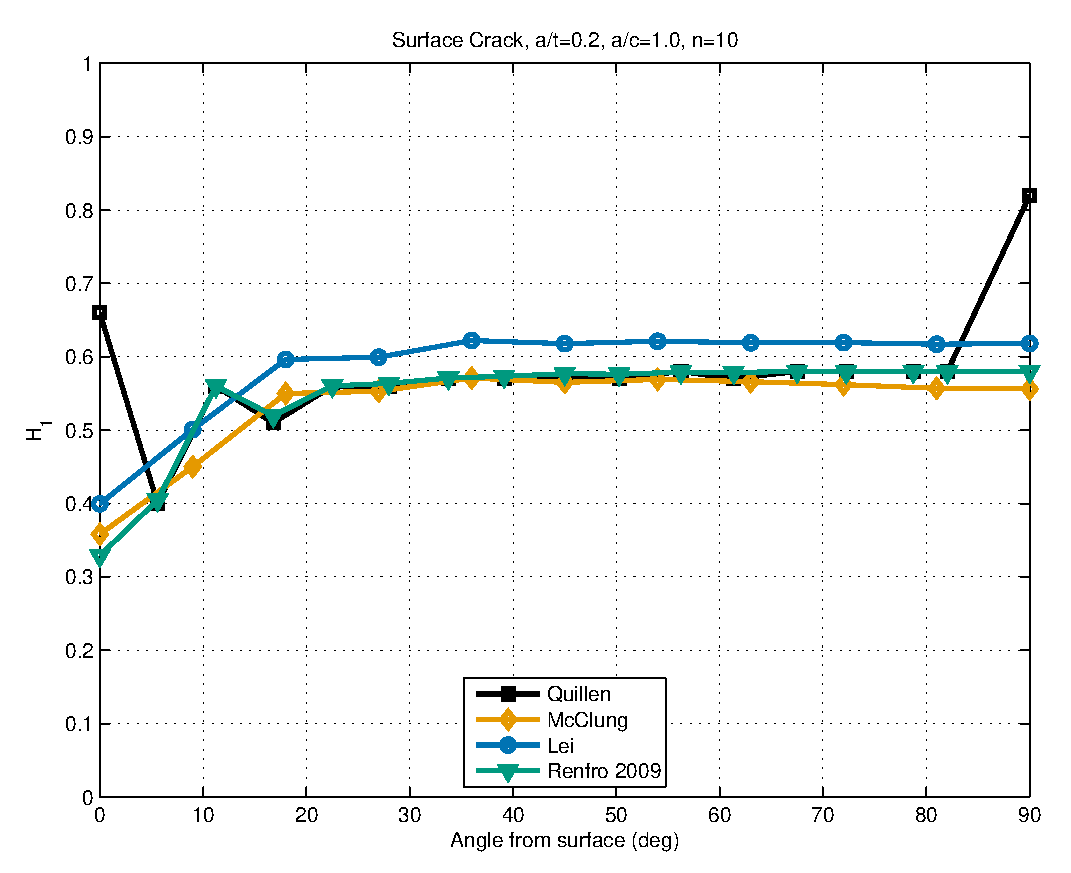
\includegraphics[width=0.5\columnwidth]{model3_rework_2009}}
\mode<presentation>{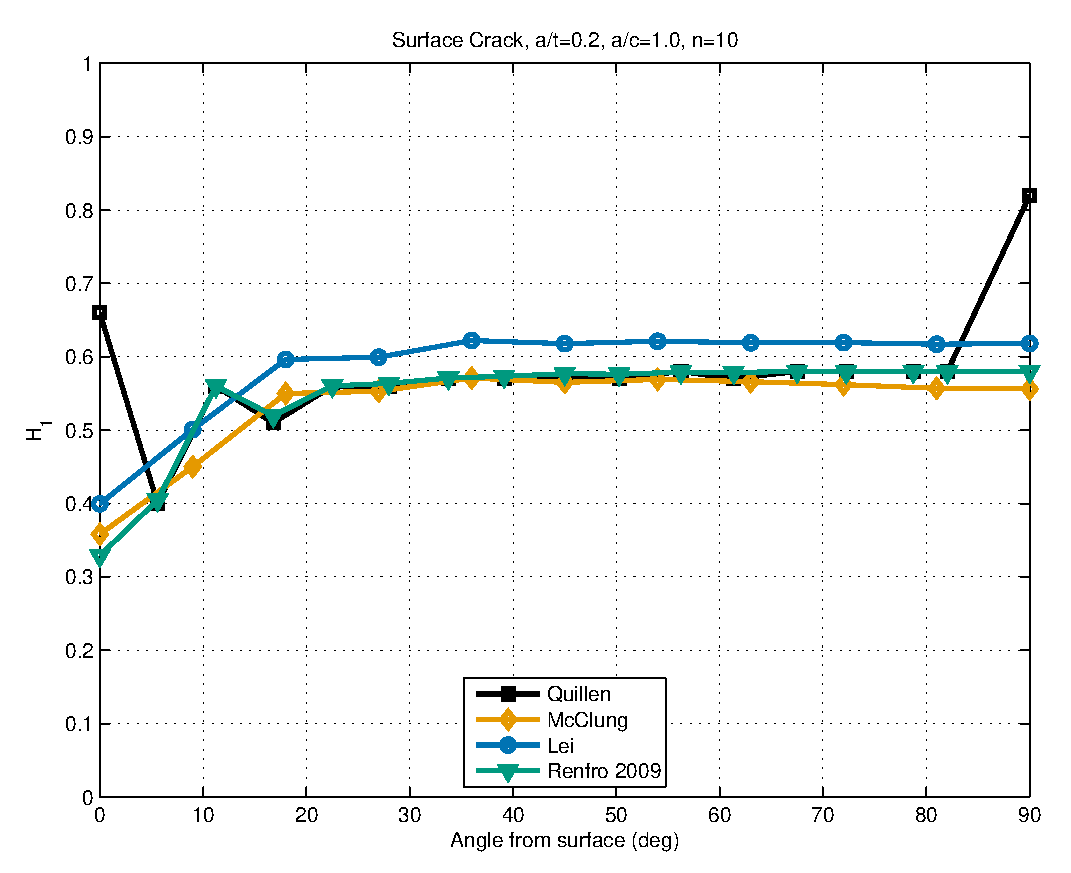
\includegraphics[width=\columnwidth]{model3_rework_2009}}
\mode<article>{\caption{\hone comparison between \citet{quillen2005} and \citet{renfro2009}, model 3, \(n=10\) \label{fig:quillen-rework-2009}}}
\end{figure}
\mode<presentation>{\end{column}\end{columns}}
\end{frame}
\note{In 2009, I ran one of Eric's models in a newer version of Abaqus with no modifications.

\vfill

Two of the three anomalies disappeared, but one remained.

\vfill

I converted his post-processing procedures from Excel macros to a more maintainable combination of Python and MATLAB.

\vfill
}

%\section{Development of Scripted Finite Element Models}

One disadvantage to the earlier finite element models is the difficulty in tracking changes to model input.
Most models are constructed interactively, which makes it difficult to isolate the critical differences between a working model and a non-working one.
Imagine having to click through every dialog box that could affect results, doing this on multiple models, and visually checking for differences in each of the material properties, boundary conditions, element types, etc.
In some cases, the user can write a plain-text file representing the model, but this can sometimes include lots of irrelevant information, or may simply contain a list of nodes and elements instead of driving variables such as mesh size parameters.

Details of the development of scripted finite element models are given in \Cref{chap:app-quillen-rework}, but the motivation can be summarized as a need to increase automation for parametric studies, to reduce opportunities for manual errors, to modularize and reduce duplicate code, and to improve tracking of changes made to models over time.
The resulting Python script was derived from an example given in the Abaqus~6.11-1 Benchmarks Manual \citeyearpar{abaqus-611-benchmarks-manual}, and can construct any of the tension models on demand, within a matter of seconds.

%Many finite element analysis software packages support the use of input files with a proprietary keyword syntax.
%Examples of this syntax include APDL (ANSYS parametric design language) and keyword syntax in Abaqus.
%Creating models with this method is more difficult for new users than with the graphical interactive method.
%However, since the keyword method is much closer to writing programs in a high-level programming language, it is much easier to isolate differences between models based off the differences in their input files.
%See \Cref{fig:material-apdl} for an example of a material property definition in APDL syntax, and \Cref{fig:material-abaqus-keyword} for the same material property definition in Abaqus keyword syntax.
%In both examples, the elastic modulus \(E\)\nomenclature[1E]{\(E\)}{elastic modulus} is defined on the first line, Poisson's ratio \(\nu\)\nomenclature[2\nu]{\(\nu\)}{Poisson's ratio} is defined on the second line, and both can be referenced wherever needed afterwards.
%
%\mode<presentation>{
%\begin{frame}
%\frametitle{Difficulty applying V\&V to finite element models}
%\begin{columns}[t]
%\begin{column}{0.45\textwidth}
%Most models
%\begin{itemize}
%\item constructed interactively in a GUI
%\item may require tedious verification of settings in every menu and dialog
%\item plain-text logs may exist
%\item logs may contain irrelevant information
%\item logs may omit critical parameters
%\end{itemize}
%\end{column}
%\begin{column}{0.45\textwidth}
%Some models
%\begin{itemize}
%\item constructed with proprietary input language
%\item allows some level of ``code verification''
%\end{itemize}
%\end{column}
%\end{columns}
%\end{frame}
%}
%\note{One thing that bothered me at the time, even though I didn't have a formal vocabulary for it, was that Eric's model was difficult to perform V\&V on.
%
%\vfill
%
%Most finite element models are like that---they're constructed interactively, with a GUI, and when (not if) errors or glitches happen, it's difficult to identify their origin.
%
%\vfill
%
%Some models (often simpler 2D ones) are constructed in an input language for the finite element program.
%
%\vfill
%
%This is an improvement in terms of code verification, but isn't always easily applied to more complex models.
%
%\vfill
%
%Eric's models were constructed in a third-party program (FEA-Crack) and analyzed in Abaqus.
%
%\vfill
%
%By 2009, we no longer had a license to FEA-Crack, and renewing it was prohibitively expensive.
%
%\vfill
%
%Though FEA-Crack used Abaqus' input language syntax, it basically wrote out a giant list of nodes and elements, making it difficult to impossible to determine why his models had anomalies at the third node.
%
%\vfill
%}
%
%\begin{frame}[containsverbatim]
%\begin{columns}[b]
%\begin{column}{0.5\textwidth}
%\begin{figure}
%\begin{lstlisting}[language={APDL}]
%! Define parameters
%E=30.0e6
%NU=0.3
%! Set material properties
%MP,EX,1,E
%MP,PRXY,1,NU
%\end{lstlisting}
%\caption{Material definition in APDL syntax \label{fig:material-apdl}}
%\end{figure}
%\end{column}
%\begin{column}{0.5\textwidth}
%\begin{figure}
%\begin{lstlisting}[language={Abaqus}]
%** Define parameters
%*PARAMETER
%E=30.0e6
%NU=0.3
%** Set material properties
%*MATERIAL, NAME=STEEL
%*ELASTIC
%<E>, <NU>
%\end{lstlisting}
%\caption{Material definition in Abaqus keyword syntax \label{fig:material-abaqus-keyword}}
%\end{figure}
%\end{column}
%\end{columns}
%\end{frame}
%\note{Here's an example of a material model definition in both ANSYS and Abaqus.
%
%\vfill
%
%They're more or less readable if you're familiar with the material property terminology, but there are some limitations.
%
%\vfill
%}
%
%One disadvantage to the APDL and Abaqus keyword languages is that both store all parameters in a single global scope.
%That is, they require any variable (for example, \verb|NU|) to have the same meaning at all places in the code, making it more difficult to describe a problem involving both Poisson's ratio (\( \nu \) in solid mechanics) and kinematic viscosity (\( \nu \) in fluid mechanics).
%Even if the variables were renamed to have distinct names (for example, \verb|PR| and \verb|KV|), the code would still require everyone using the set of code to agree on one set of names, making code sharing throughout a research community more difficult.
%
%\mode<presentation>{
%\begin{frame}
%\frametitle{Alternatives to proprietary syntax}
%\begin{columns}[t]
%\begin{column}{0.45\textwidth}
%Proprietary languages:
%\begin{itemize}
%\item global variable scope
%\item rudimentary data types
%\item no user-defined functions
%\item syntax can be cryptic (written by engineers)
%\end{itemize}
%\end{column}
%\begin{column}{0.45\textwidth}
%Wishlist for improved language:
%\begin{itemize}
%\item local variable scope
%\item user-defined data structures
%\item user-defined functions
%\item reuse existing syntax (written by computer scientists)
%\end{itemize}
%\end{column}
%\end{columns}
%\end{frame}
%}
%\note{Compared to more general-purpose languages, the proprietary input syntax normally puts all variables into a single global scope, so that the variable NU can mean one and only one thing for the entire code.
%
%\vfill
%
%They normally only support simple numeric and string variables, lack easy definition of functions, and have arbitrary syntax.
%
%\vfill
%
%Removing each of these restrictions would have several benefits in creating models.
%
%\vfill
%
%}
%
%Abaqus has supported a second input syntax since at least version 6.2---writing models in Python.
%Python is a dynamic general-purpose language used for a variety of different applications.
%It allows for the creation of functions and modules for code reuse, and supports user-defined data structures to pass data around a program.
%An example of a material property definition in Abaqus Python scripting syntax is shown in \Cref{fig:material-abaqus-python}.
%\begin{frame}[containsverbatim]
%\begin{figure}
%\begin{lstlisting}
%def setMaterial(model, E=200e9, nu=0.3): # a function
%    model.Material(name='Steel')
%    model.materials['Steel'].Elastic(table=((E, nu), ))
%    # function ends here, main program follows
%
%elasticModulus=30e6 # define parameters
%PoissonRatio=0.3
%# call functions to create model, set material
%myModel = createModel(modelName='McClung-1')
%setMaterial(E=elasticModulus,
%            nu=PoissonRatio,
%            model=myModel)
%\end{lstlisting}
%\caption{Material definition in Abaqus Python syntax \label{fig:material-abaqus-python}}
%\end{figure}
%\end{frame}
%\note{Abaqus has had a second language option for building models for several years, and that's Python.
%
%\vfill
%
%Though the material definition shown here is much more verbose than the previous ones, it demonstrates several improvements in the language including
%
%\vfill
%
%user-defined functions,
%
%\vfill
%
%local variables,
%
%\vfill
%
%object-oriented features,
%
%\vfill
%
%richer datatypes,
%
%\vfill
%
%default function parameters,
%
%\vfill
%
%and arranging function parameters in any convenient order.
%
%\vfill
%}
%
%Though the Python version of the material property definition is more verbose than either of the keyword versions of the definition, it is arguably more readable to an infrequent user.
%The code also demonstrates four valuable features of Python scripting: the ability to create user-defined functions, the existence of a local variable scope for functions (so that parameters are not defined in a global scope by default), the ability to pass named parameters to functions in any order, and the ability to have default values for any parameters not defined in the function call.
%
%The existence of functions is critical for a program to be easily maintained: if an error is found in a function, it can be corrected once, and that correction automatically propagates everywhere the function was used.
%If an error is found in an equation that has been copied and pasted repeatedly (due to a lack of functions in the language), the error must be corrected everywhere the equation exists.
%
%Local parameter scopes are very helpful: they remove the requirement that a variable name have one and only one meaning throughout a body of code, and throughout any code that will ever be used with it.
%Default values for parameters and the ability to use named parameters in any order are convenient.
%Both of these features enable a research community to coordinate on what set of parameters needs to be passed to a function, and what result that function returns, but places no restrictions on what the parameters or result should be named.
%This allows the research community to be more loosely coordinated, and for them to share code more easily with fewer modifications.
%
%\mode<presentation>{
%\begin{frame}
%\frametitle{Abaqus scripting with Python}
%\begin{columns}[t]
%\begin{column}{0.45\textwidth}
%Advantages:
%\begin{itemize}
%\item reusable functions and modules
%\item local variable scope
%\item default values for function parameters
%\item broader set of data types (lists, dictionaries)
%\end{itemize}
%\end{column}
%\begin{column}{0.45\textwidth}
%Results:
%\begin{itemize}
%\item program to model elliptical surface cracks
%\item 1250 lines of code (1100 lines in modules)
%\item \SI{66}{\kilo\byte} disk space for code versus \SI{1}{\mega\byte} for a single input file
%\item any model generated within \SI{10}{\second} on a laptop
%\end{itemize}
%\end{column}
%\end{columns}
%\end{frame}
%}
%Working from a basic Python program for elliptical surface cracks given in the Abaqus~6.11-1 Benchmarks Manual \citeyearpar{abaqus-611-benchmarks-manual}, a new program has been developed to reliably and repeatably analyze surface cracks in plates for any valid combination of plate geometry, crack geometry, material properties, and remote pressures.
%This program includes functions for:
%\begin{itemize}
%\item creation of plate geometry,
%\item creation of an elliptical path representing the crack front,
%\item sweeping two
%circular
%%square
%profiles along the elliptical path to create regions for singularity elements and transitional elements near the crack front,
%\item assembling the plate and swept profiles into a single assembly,
%\item partitioning the plate to enable focused hexahedral meshing throughout the plate,
%\item assignment of simple elastic or Ramberg-Osgood elastic-plastic material properties,
%\item creation of geometry sets for the traction surface, symmetry planes, and crack front,
%\item definition of contour integral \J along the crack front,
%\item assignment of mesh sizes (both default and exceptions along specific edges,
%\item meshing the model regions with singularity elements, transitional elements, or regular hexahedral elements,
%\item creation of load step and boundary conditions,
%\item creation of history output requests to track values along the crack front as appropriate (\J for elastic-plastic models; \J, \K and tangential stress for elastic models),
%\item creation of job input file,
%\item submission of input file for analysis,
%\item reading \J values from the resulting Abaqus output database (ODB)\nomenclature[1O]{ODB}{Abaqus output database},
%\item converting the \J values into \hone values analogous to those in \Cref{eq:h1mcclung}, and
%\item writing \hone values and crack node coordinates to a text file.
%\end{itemize}
%\note{In the end, using Python instead of the Abaqus input language syntax, I was able to replace Eric's use of FEA-Crack with my own program.
%
%\vfill
%
%It's about 1250 lines of code, but 1100 of those lines are factored out into reusable modules, suitable for modeling any elliptical crack problem.
%
%\vfill
%
%Any given model can be generated within 10 seconds on a regular laptop, and any changes to the code can be easily tracked for long-term verification and validation studies.
%
%\vfill
%
%Examples of the models created with this program follow.
%
%\vfill
%}
%
%% 280 lines in main file (includes 160 in seed definitions).
%% 360 lines in generic_crack_functions
%% 10 lines in model_geometry
%% 560 lines in rectangular_topology
%% 30 in pprint_table
%
%The complete program contains approximately 1250 lines of Python code and comments (a total of \SI{66}{\kilo\byte} of disk space), with 1100 lines separated into reusable modules or libraries that can be used for any semi-elliptical crack model.
%By comparison, a small input file (approximately \num{2300} elements and \num{11000} nodes) may contain over \num{17000} lines and over \SI{1}{\mega\byte} of disk space.
%Any model and its corresponding Abaqus input file can be generated within \SI{10}{\second} on an Intel Core2 Duo laptop, enabling quick generation of a set of models to be solved on a high-performance compute cluster or the laptop itself as needed.
%Examples of two of the new models are shown in \Crefrange{fig:model1-assembly}{fig:model9-assembly}.
%The text file containing node numbers, coordinates, and \hone values can be imported into MATLAB, and graphs can be created.
%The additional automation reduces opportunities for random errors in copying and pasting results, inconsistent parameter changes, and related issues.
%
%\begin{frame}
%  \begin{figure}
%    \centering
%    \mode<article>{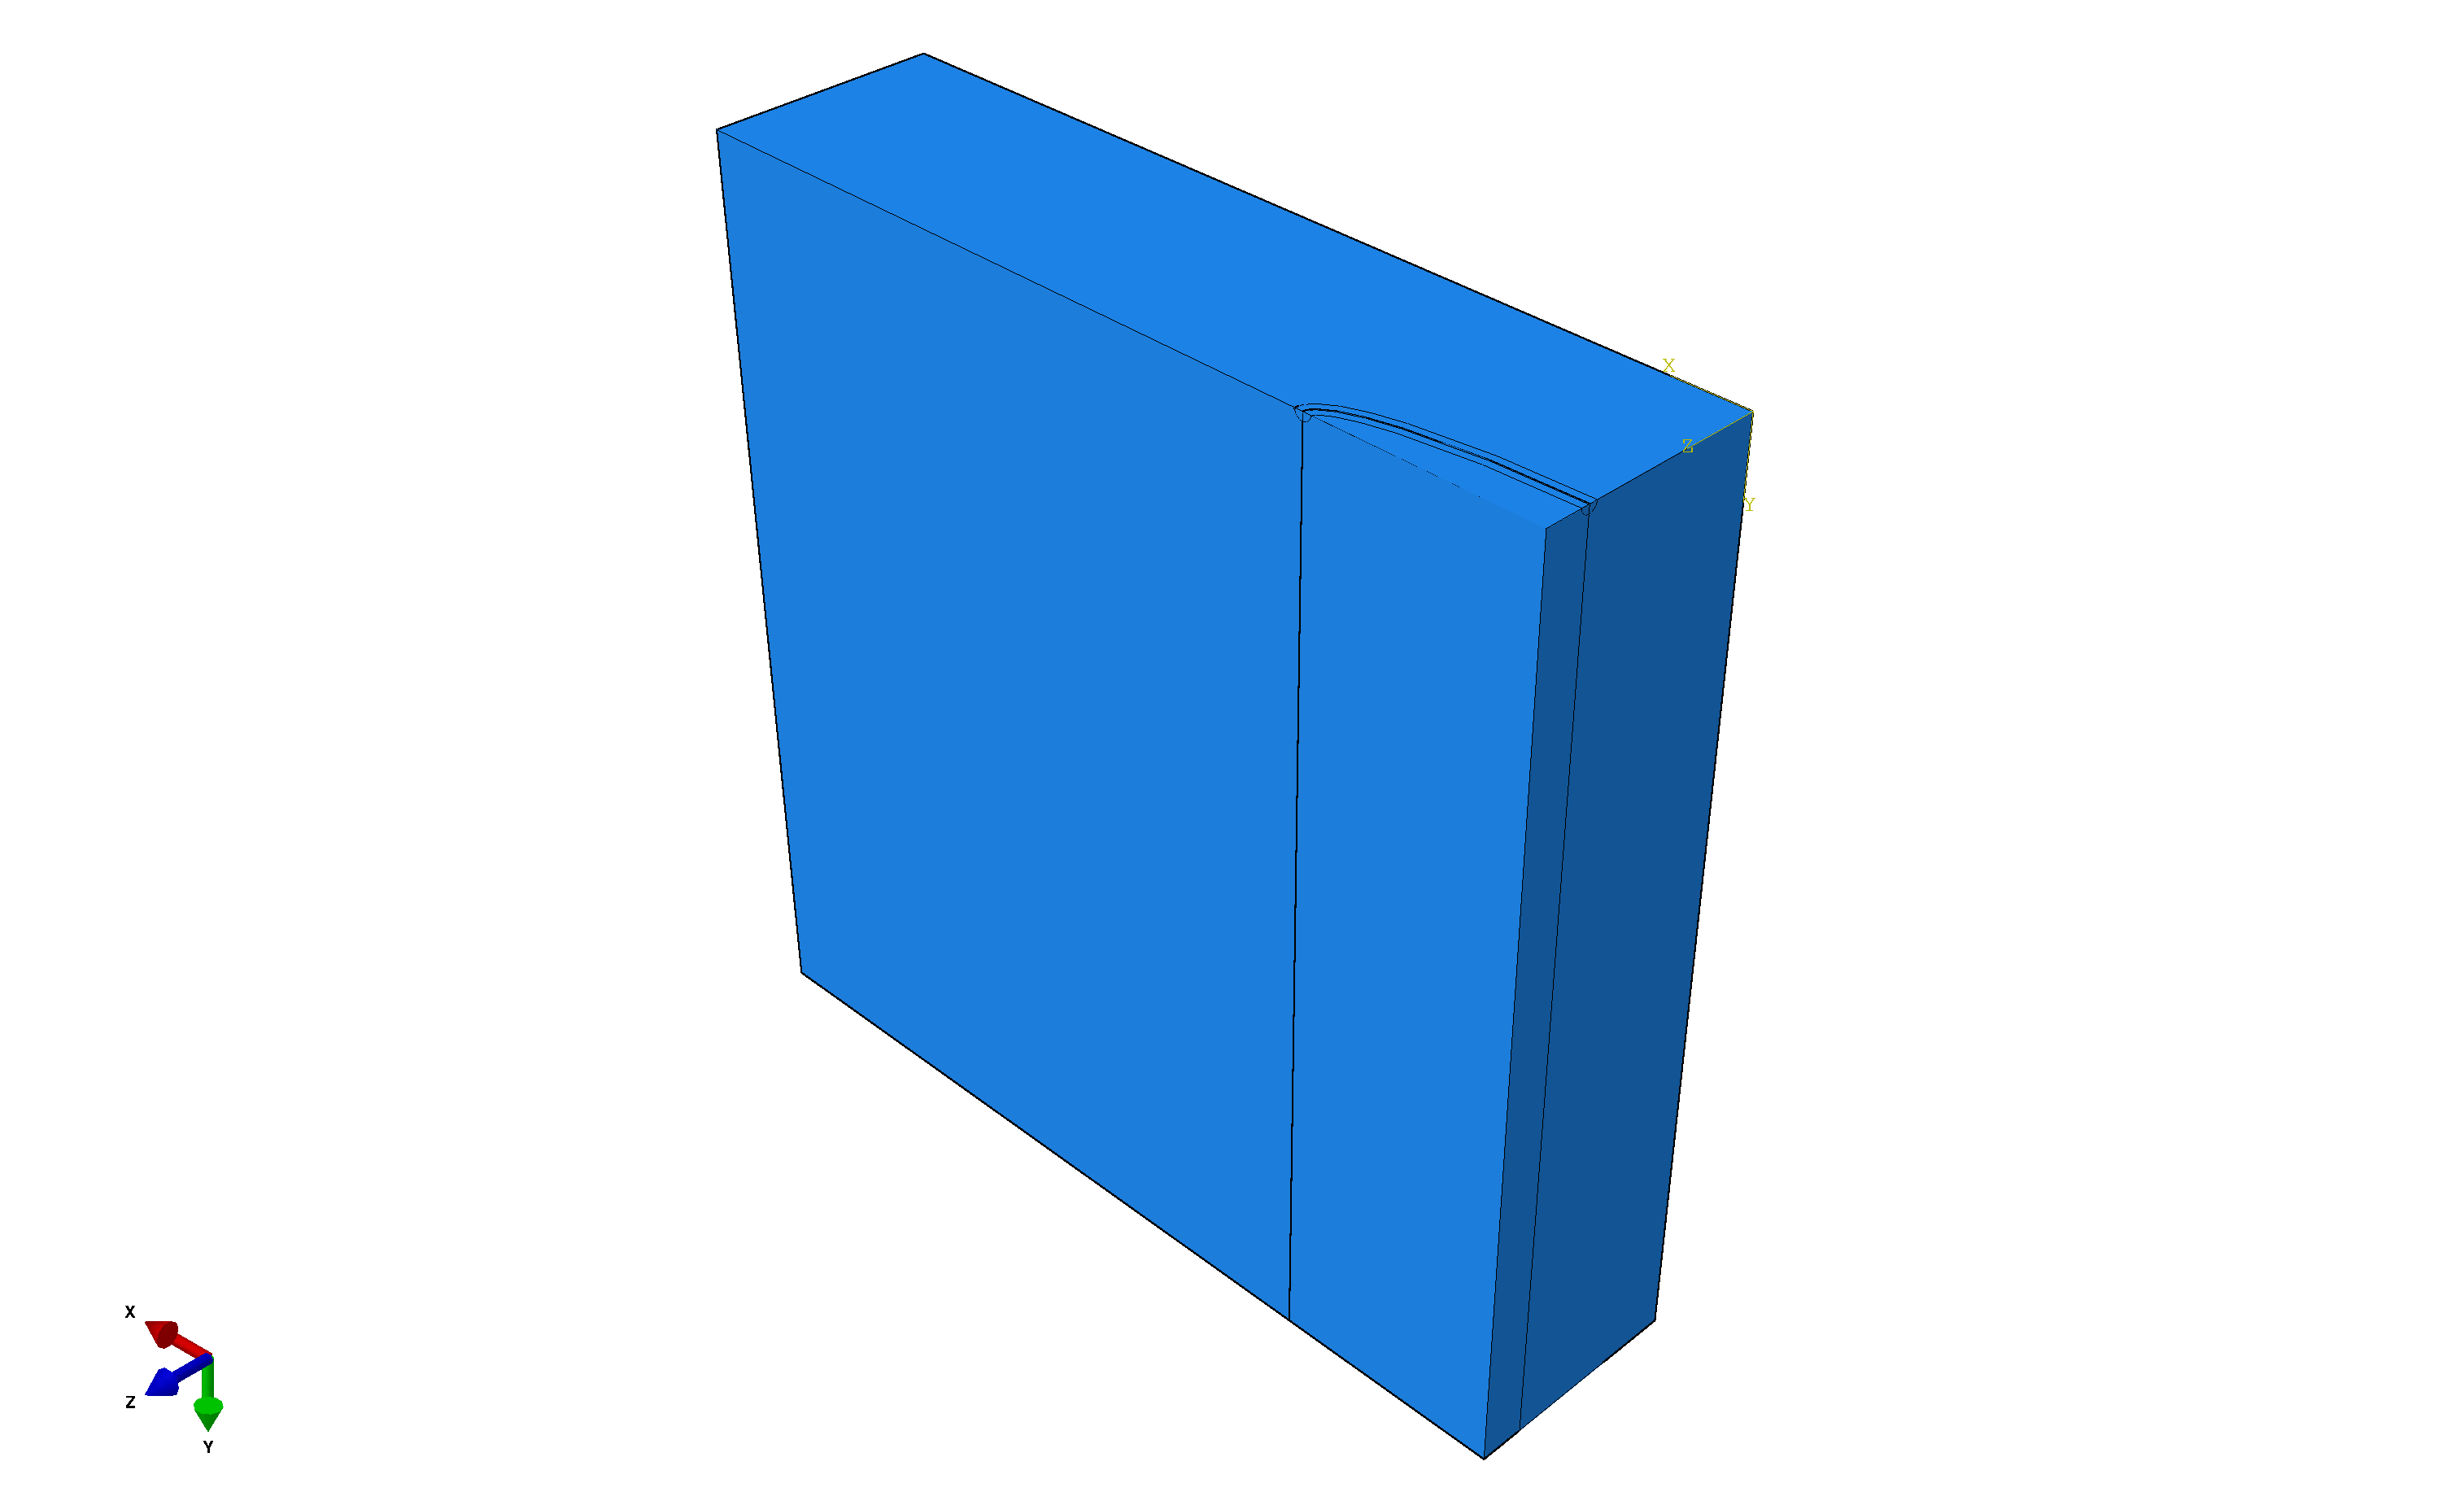
\includegraphics[width=\columnwidth]{model1-assembly}}
%    \mode<presentation>{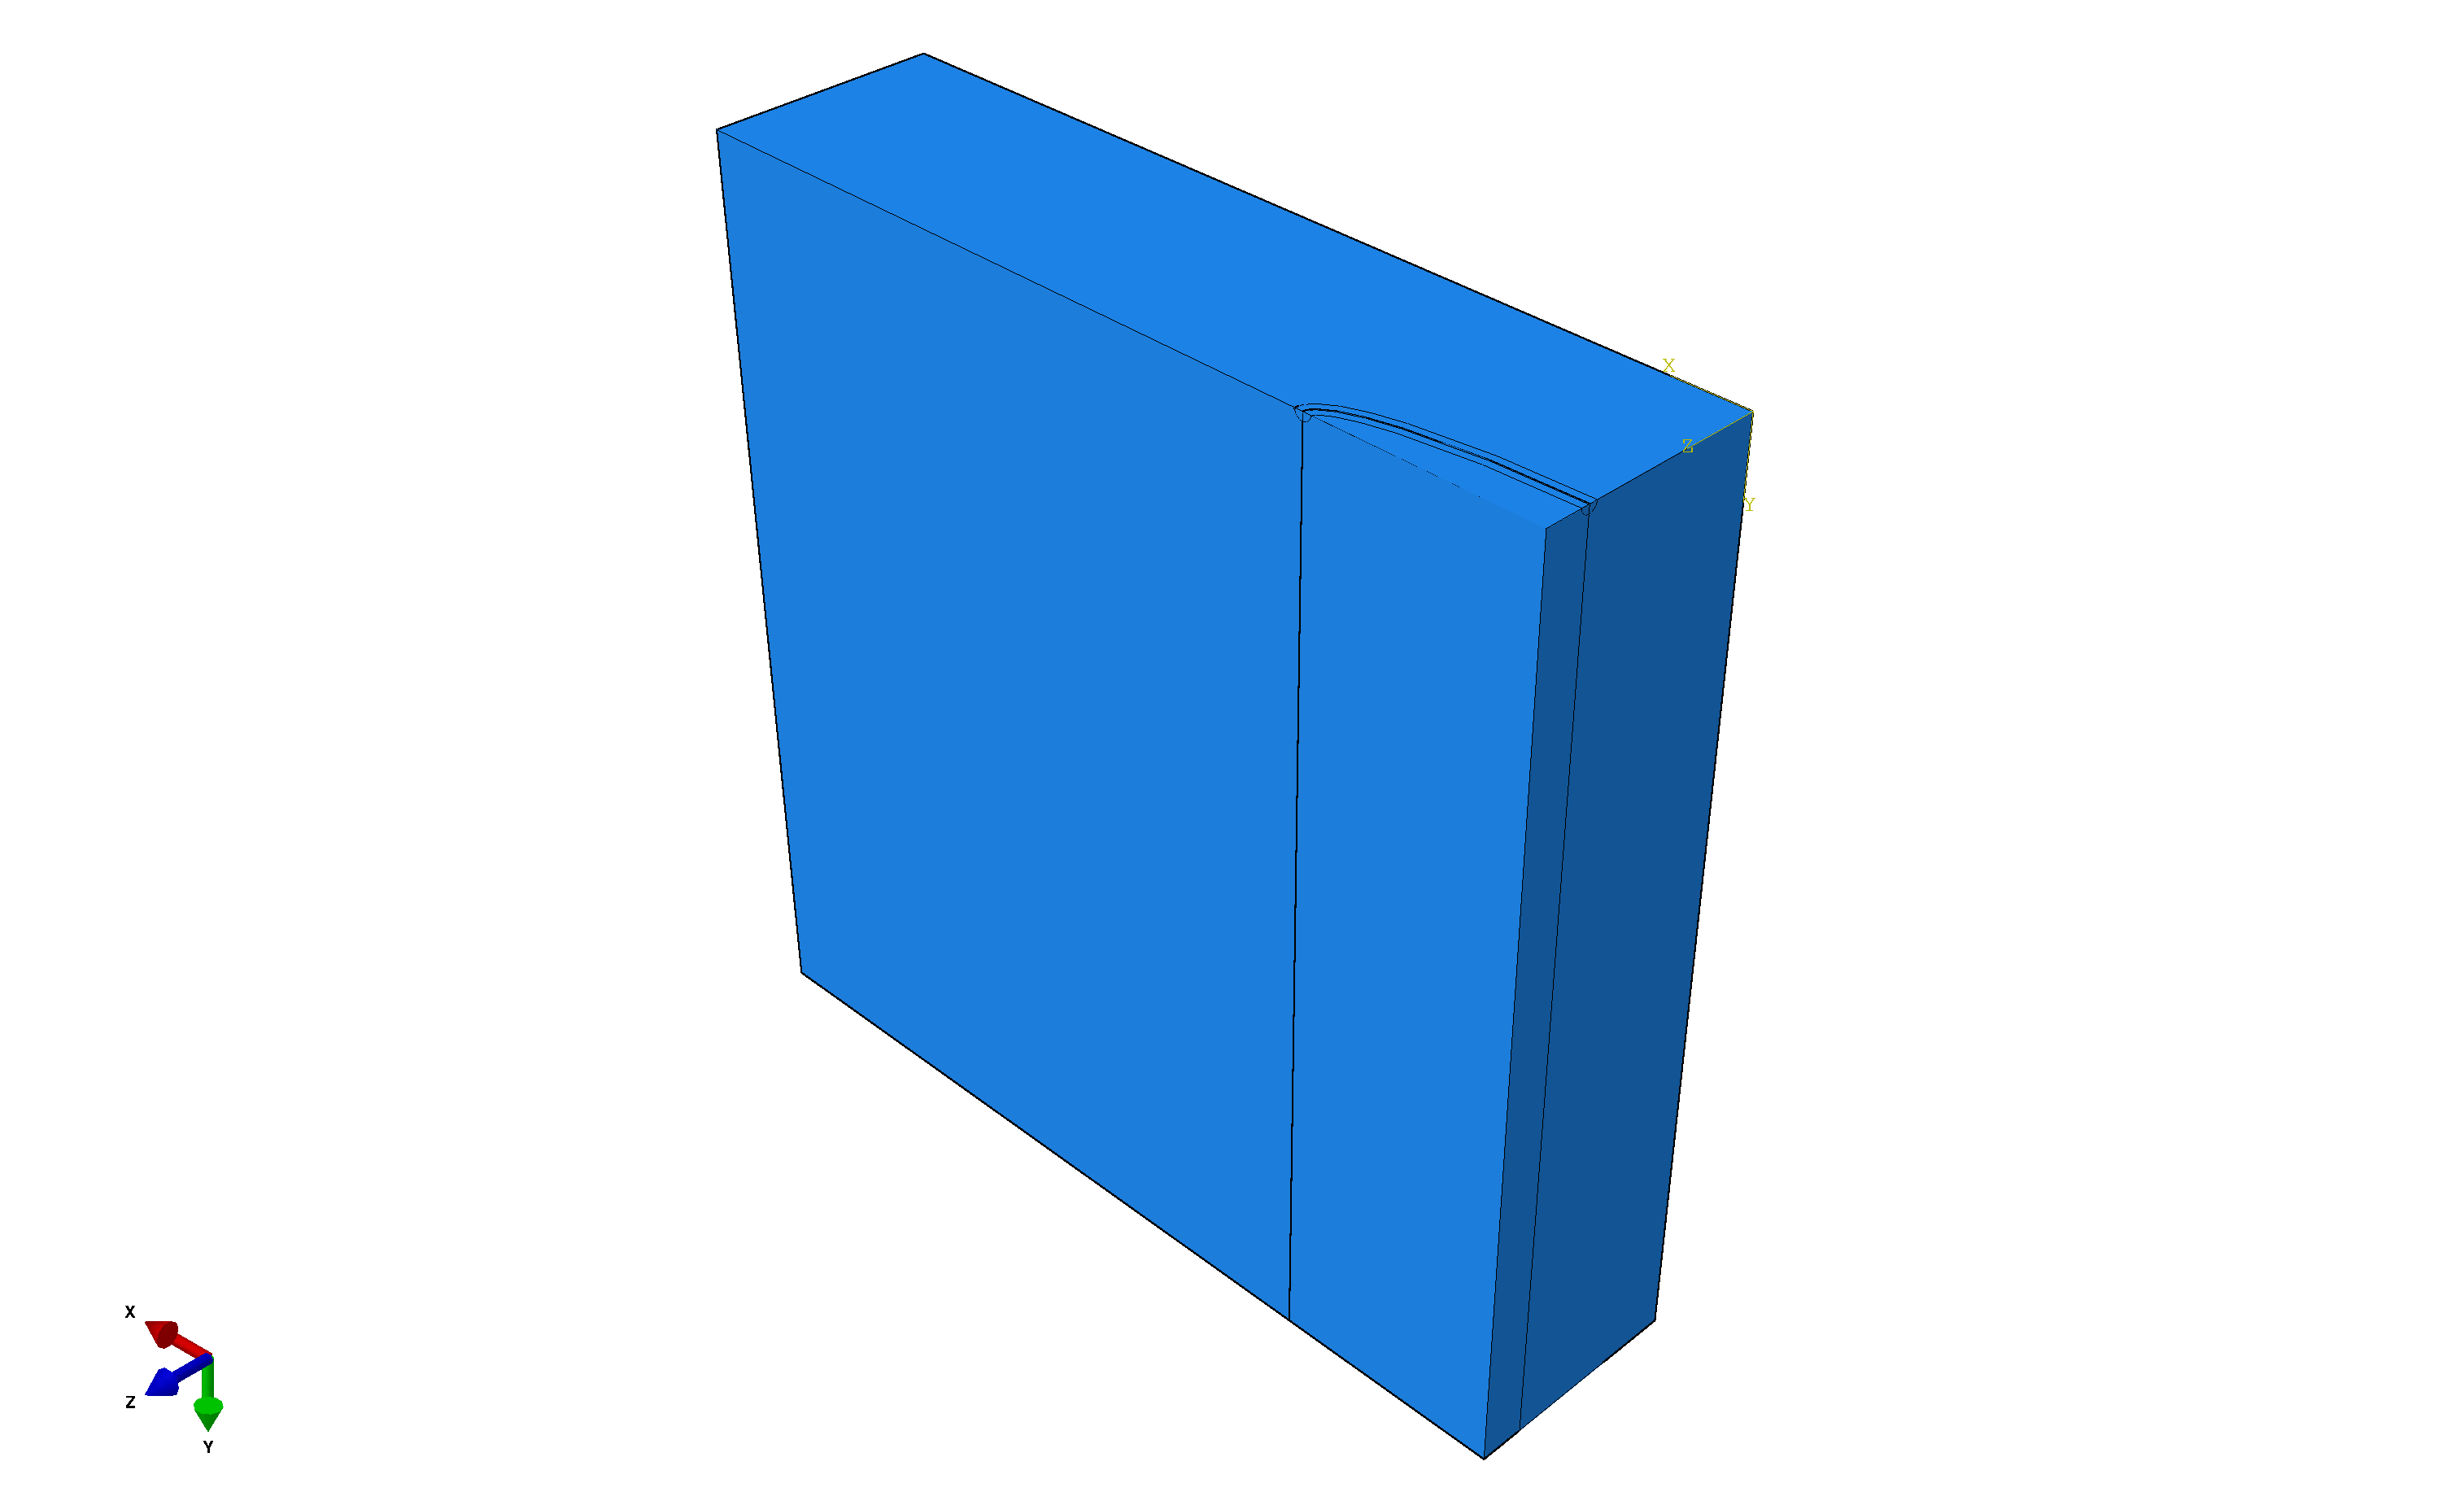
\includegraphics[width=0.7\columnwidth]{model1-assembly}}
%    \caption{McClung et al. model 1\label{fig:model1-assembly}}
%  \end{figure}
%\end{frame} \note{Model 1 is a very shallow, highly elliptical crack.}
%\begin{frame}
%  \begin{figure}
%    \centering
%    \mode<article>{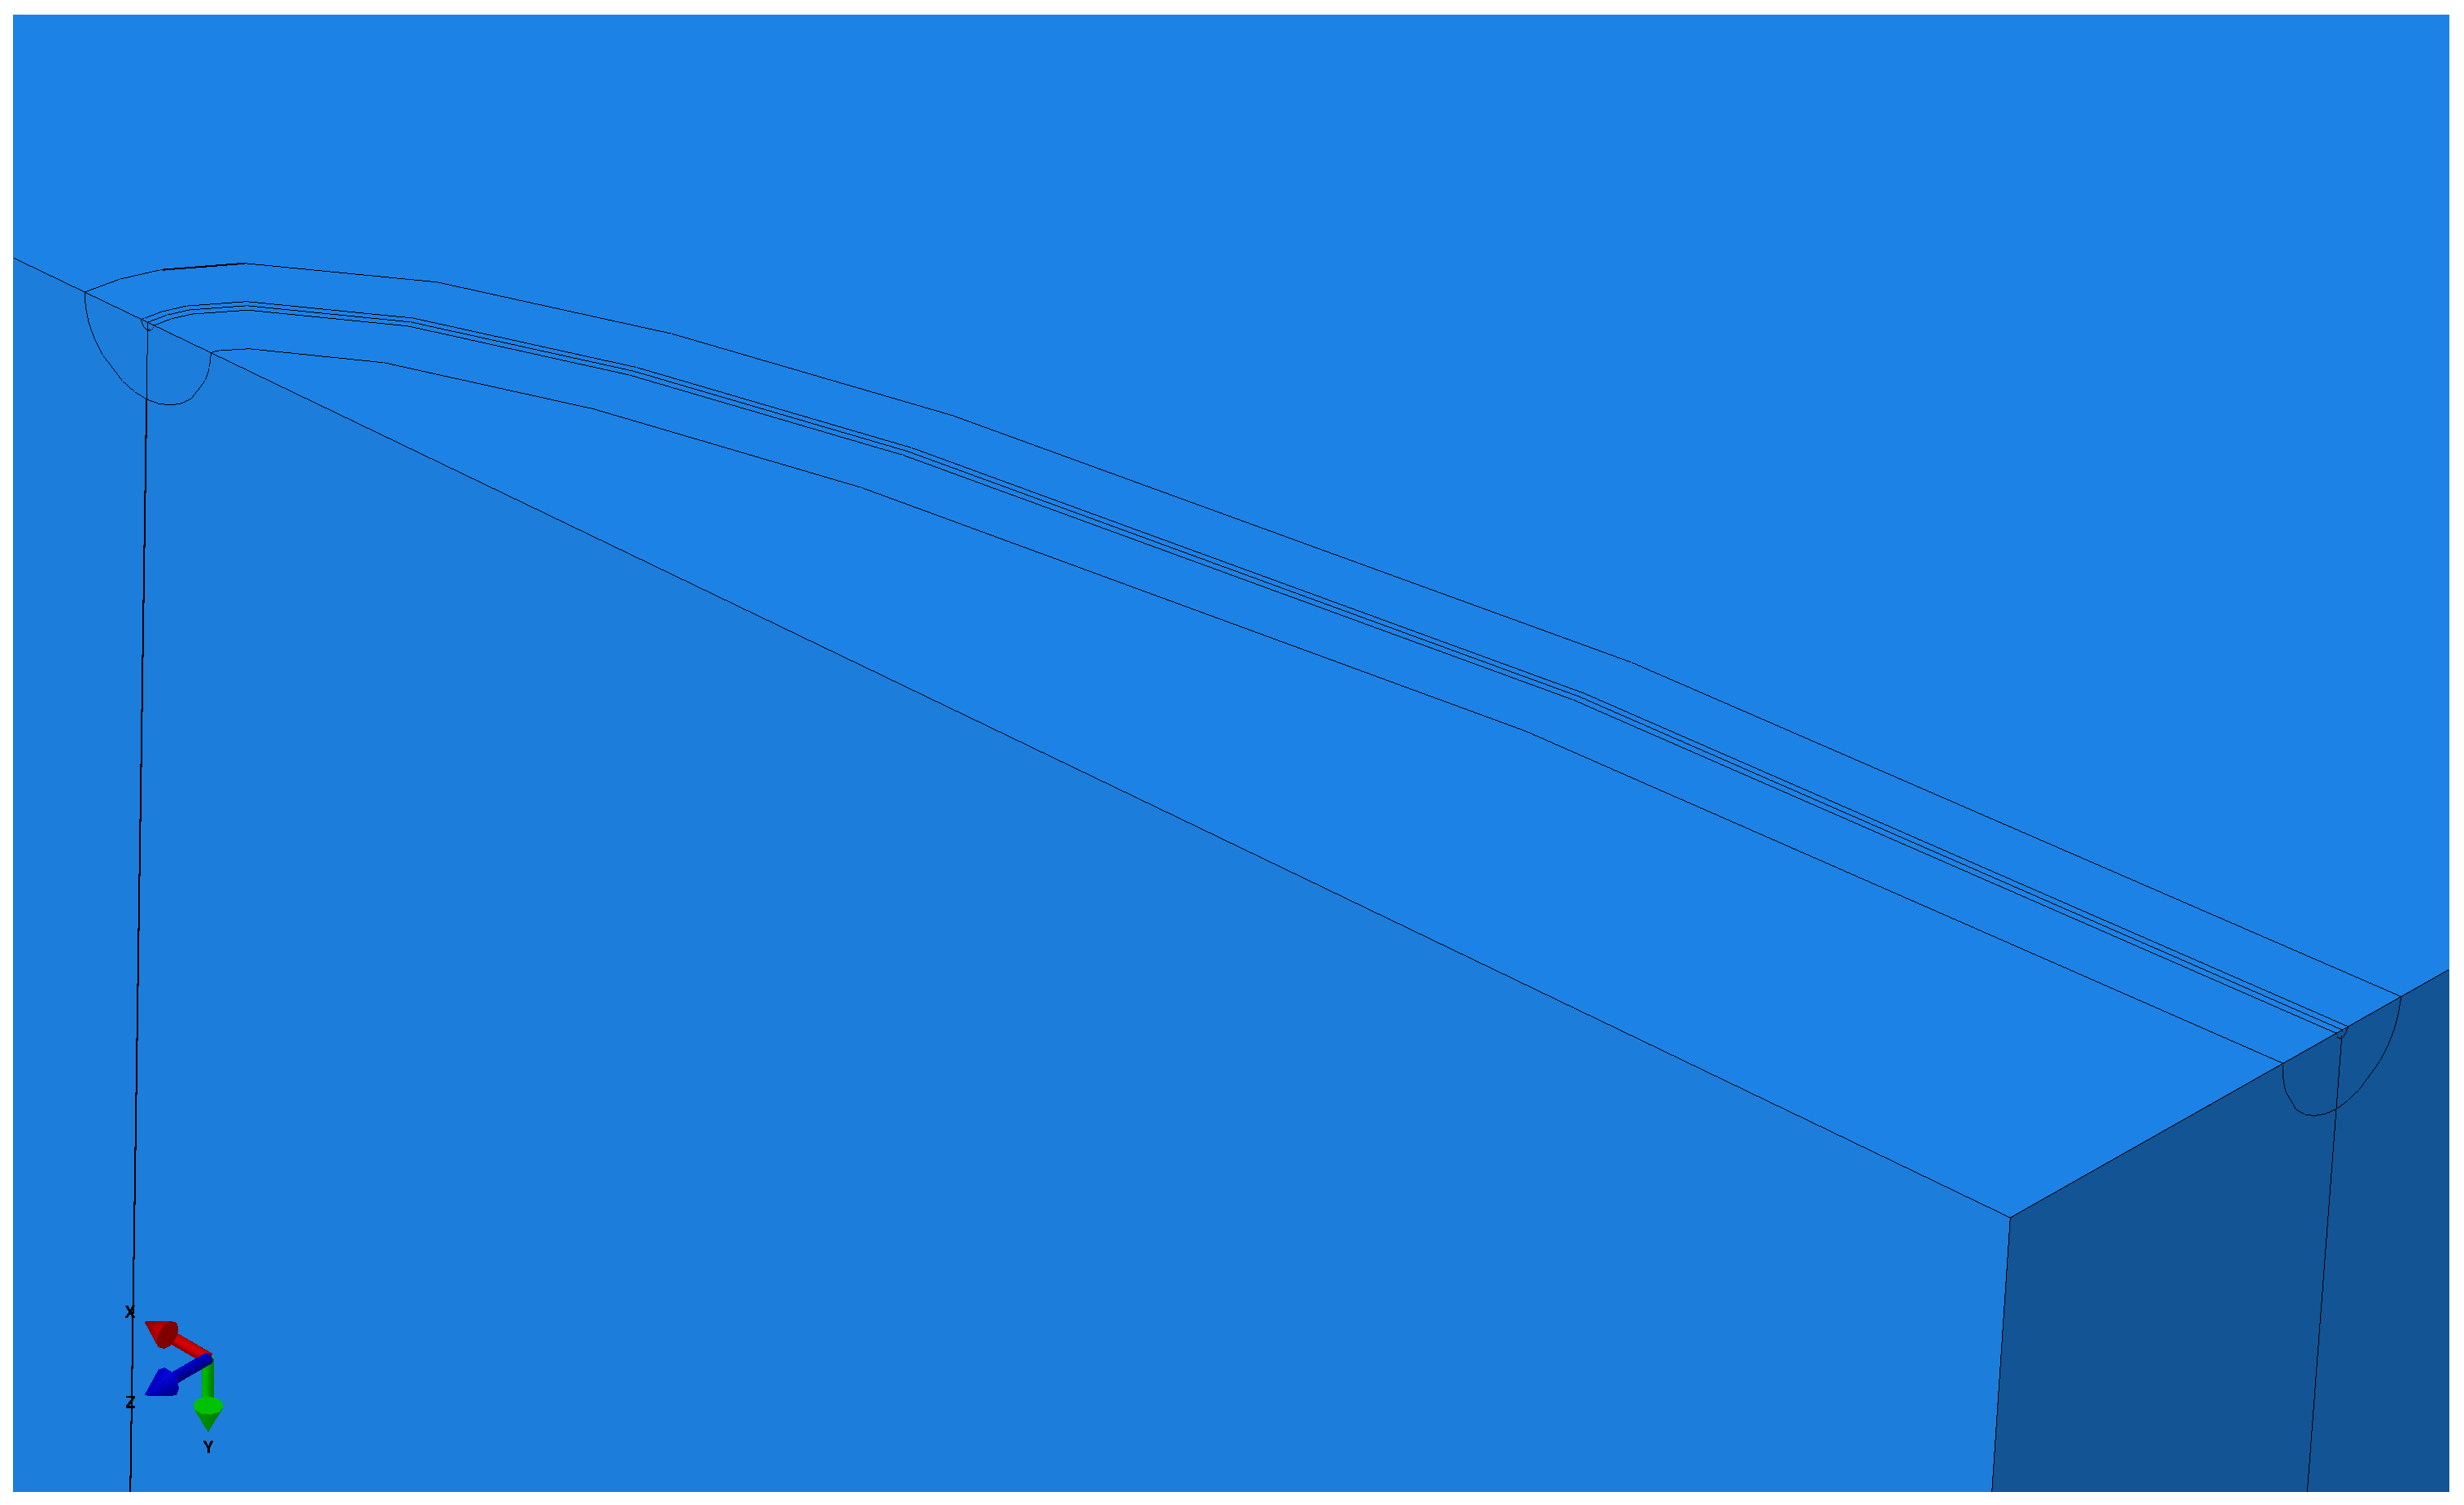
\includegraphics[width=\columnwidth]{model1-assembly-zoomed}}
%    \mode<presentation>{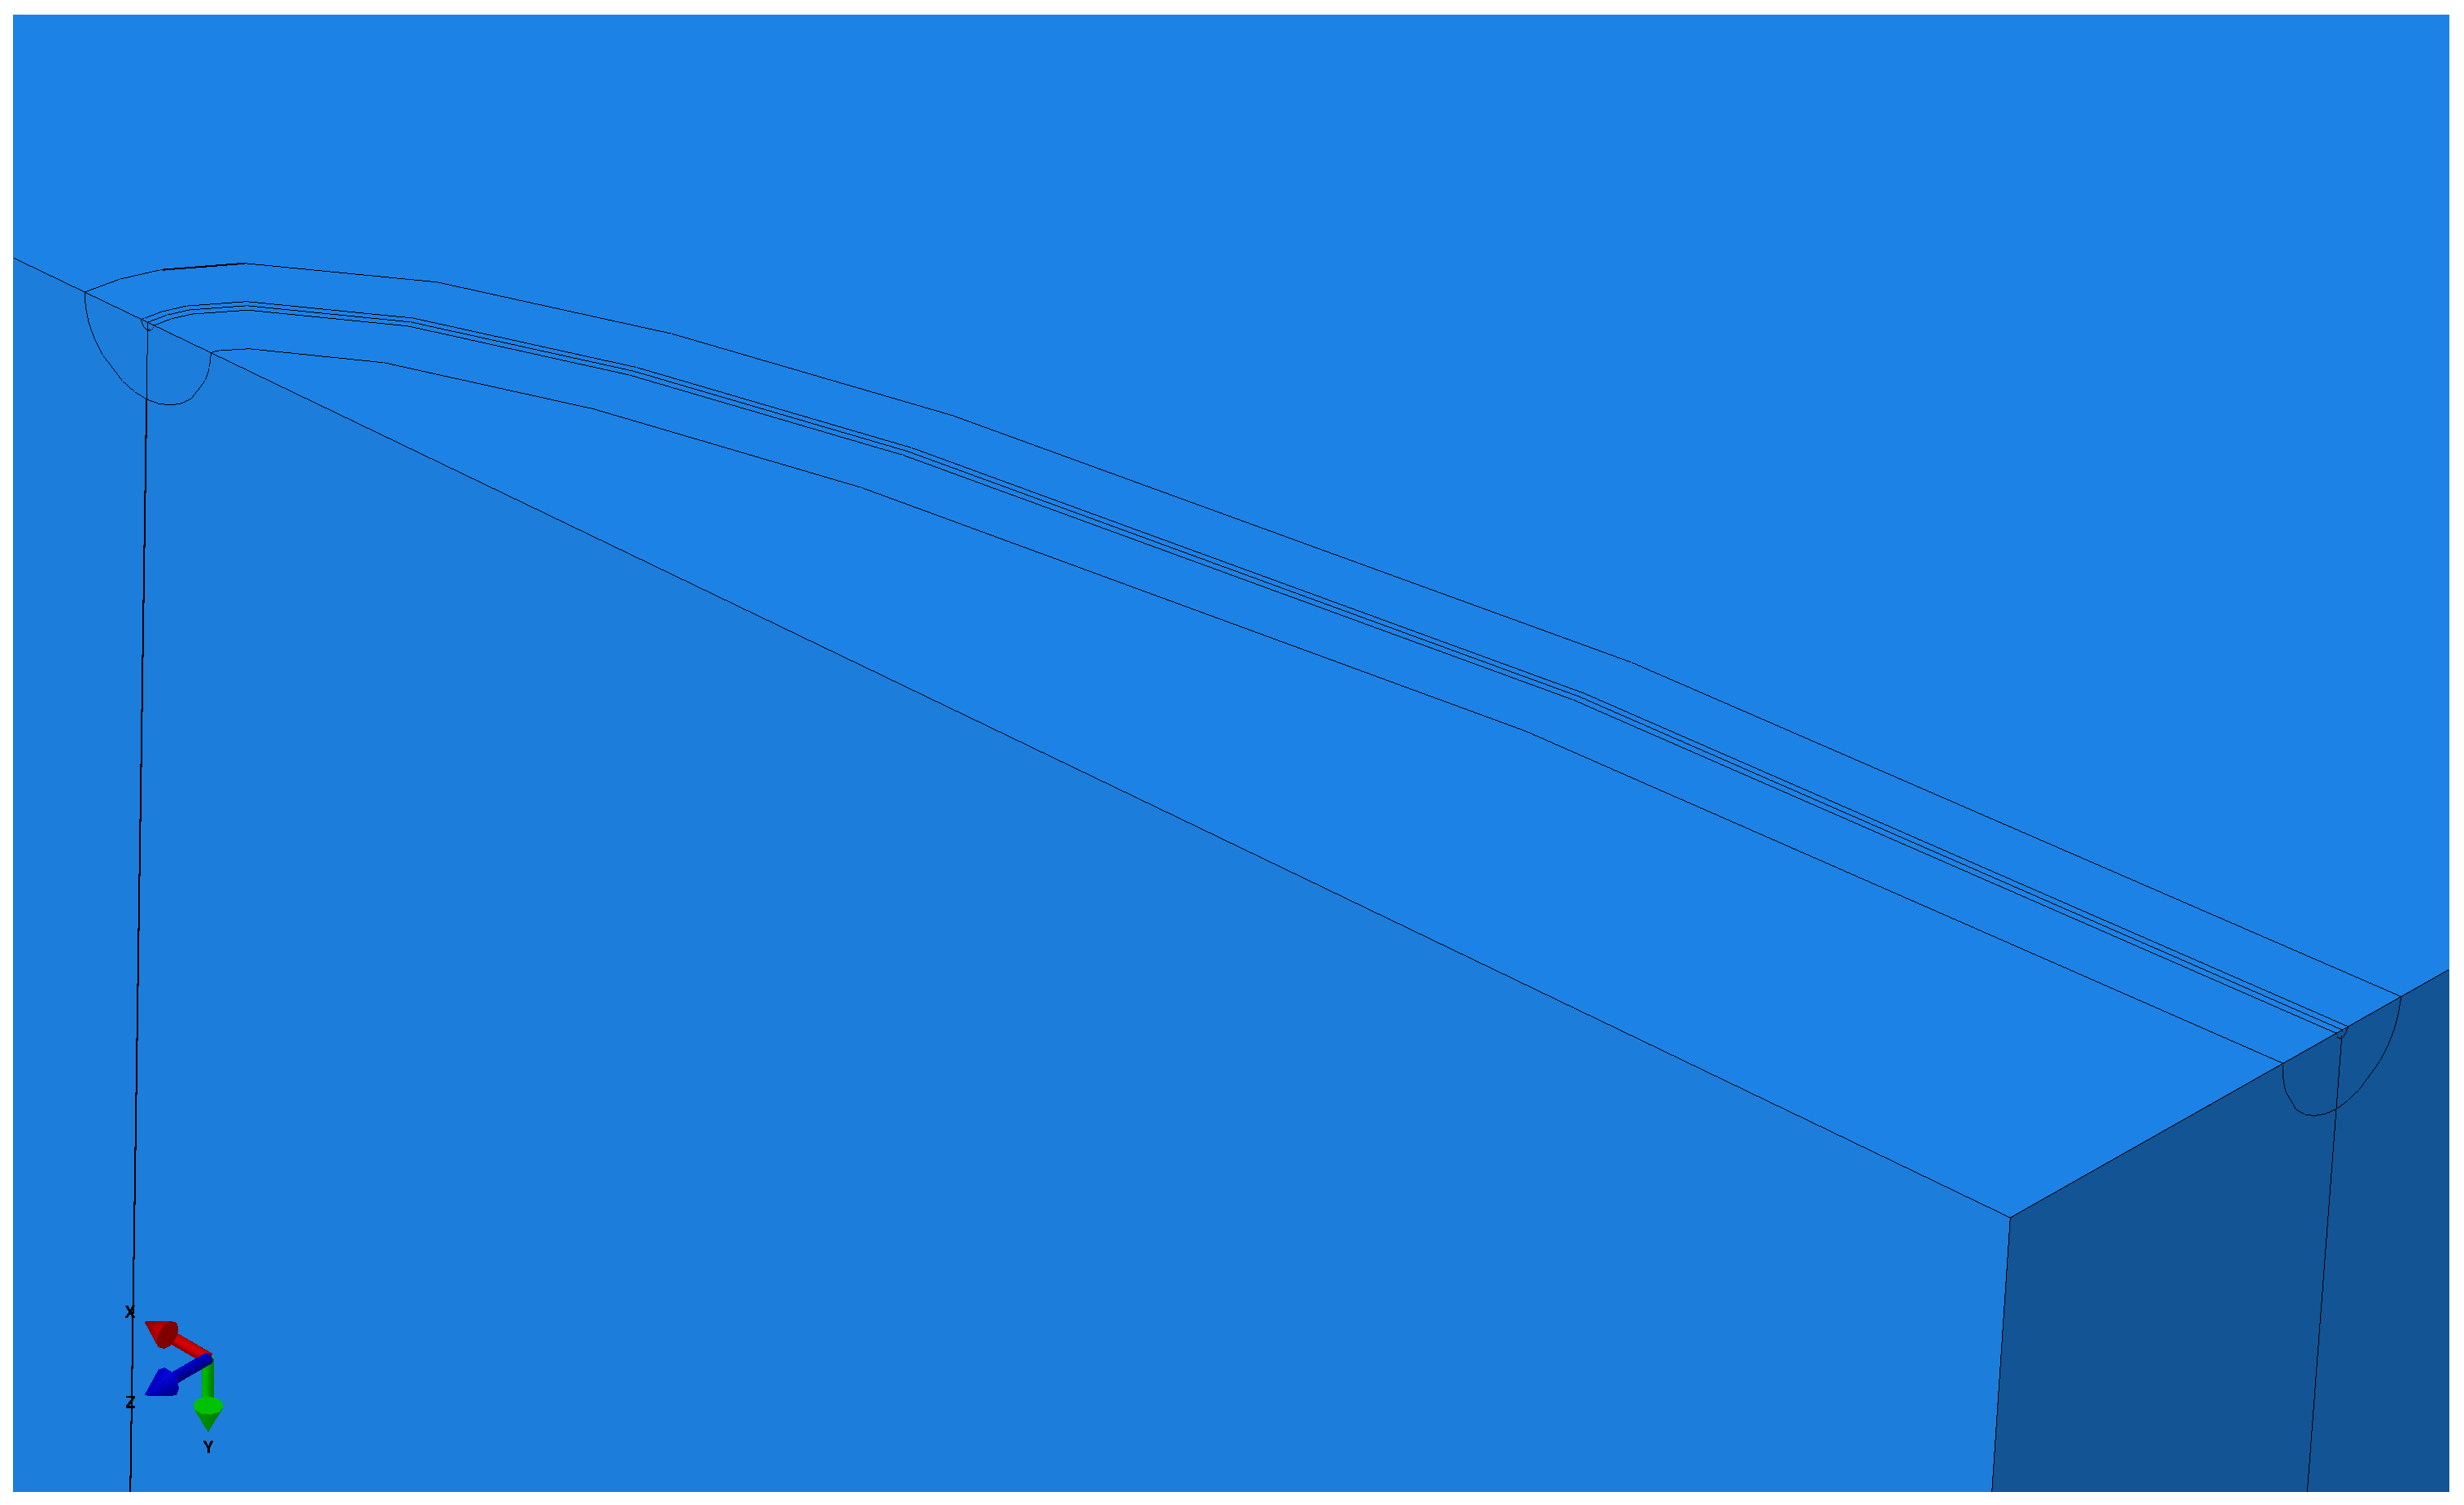
\includegraphics[width=0.7\columnwidth]{model1-assembly-zoomed}}
%    \caption{McClung et al. model 1 crack front detail\label{fig:model1-assembly-zoomed}}
%  \end{figure}
%\end{frame} \note{Zooming in on the crack front, you can see the creation of concentric regions for the crack tip and surrounding material.}
%\begin{frame}
%  \begin{figure}
%    \centering
%    \mode<article>{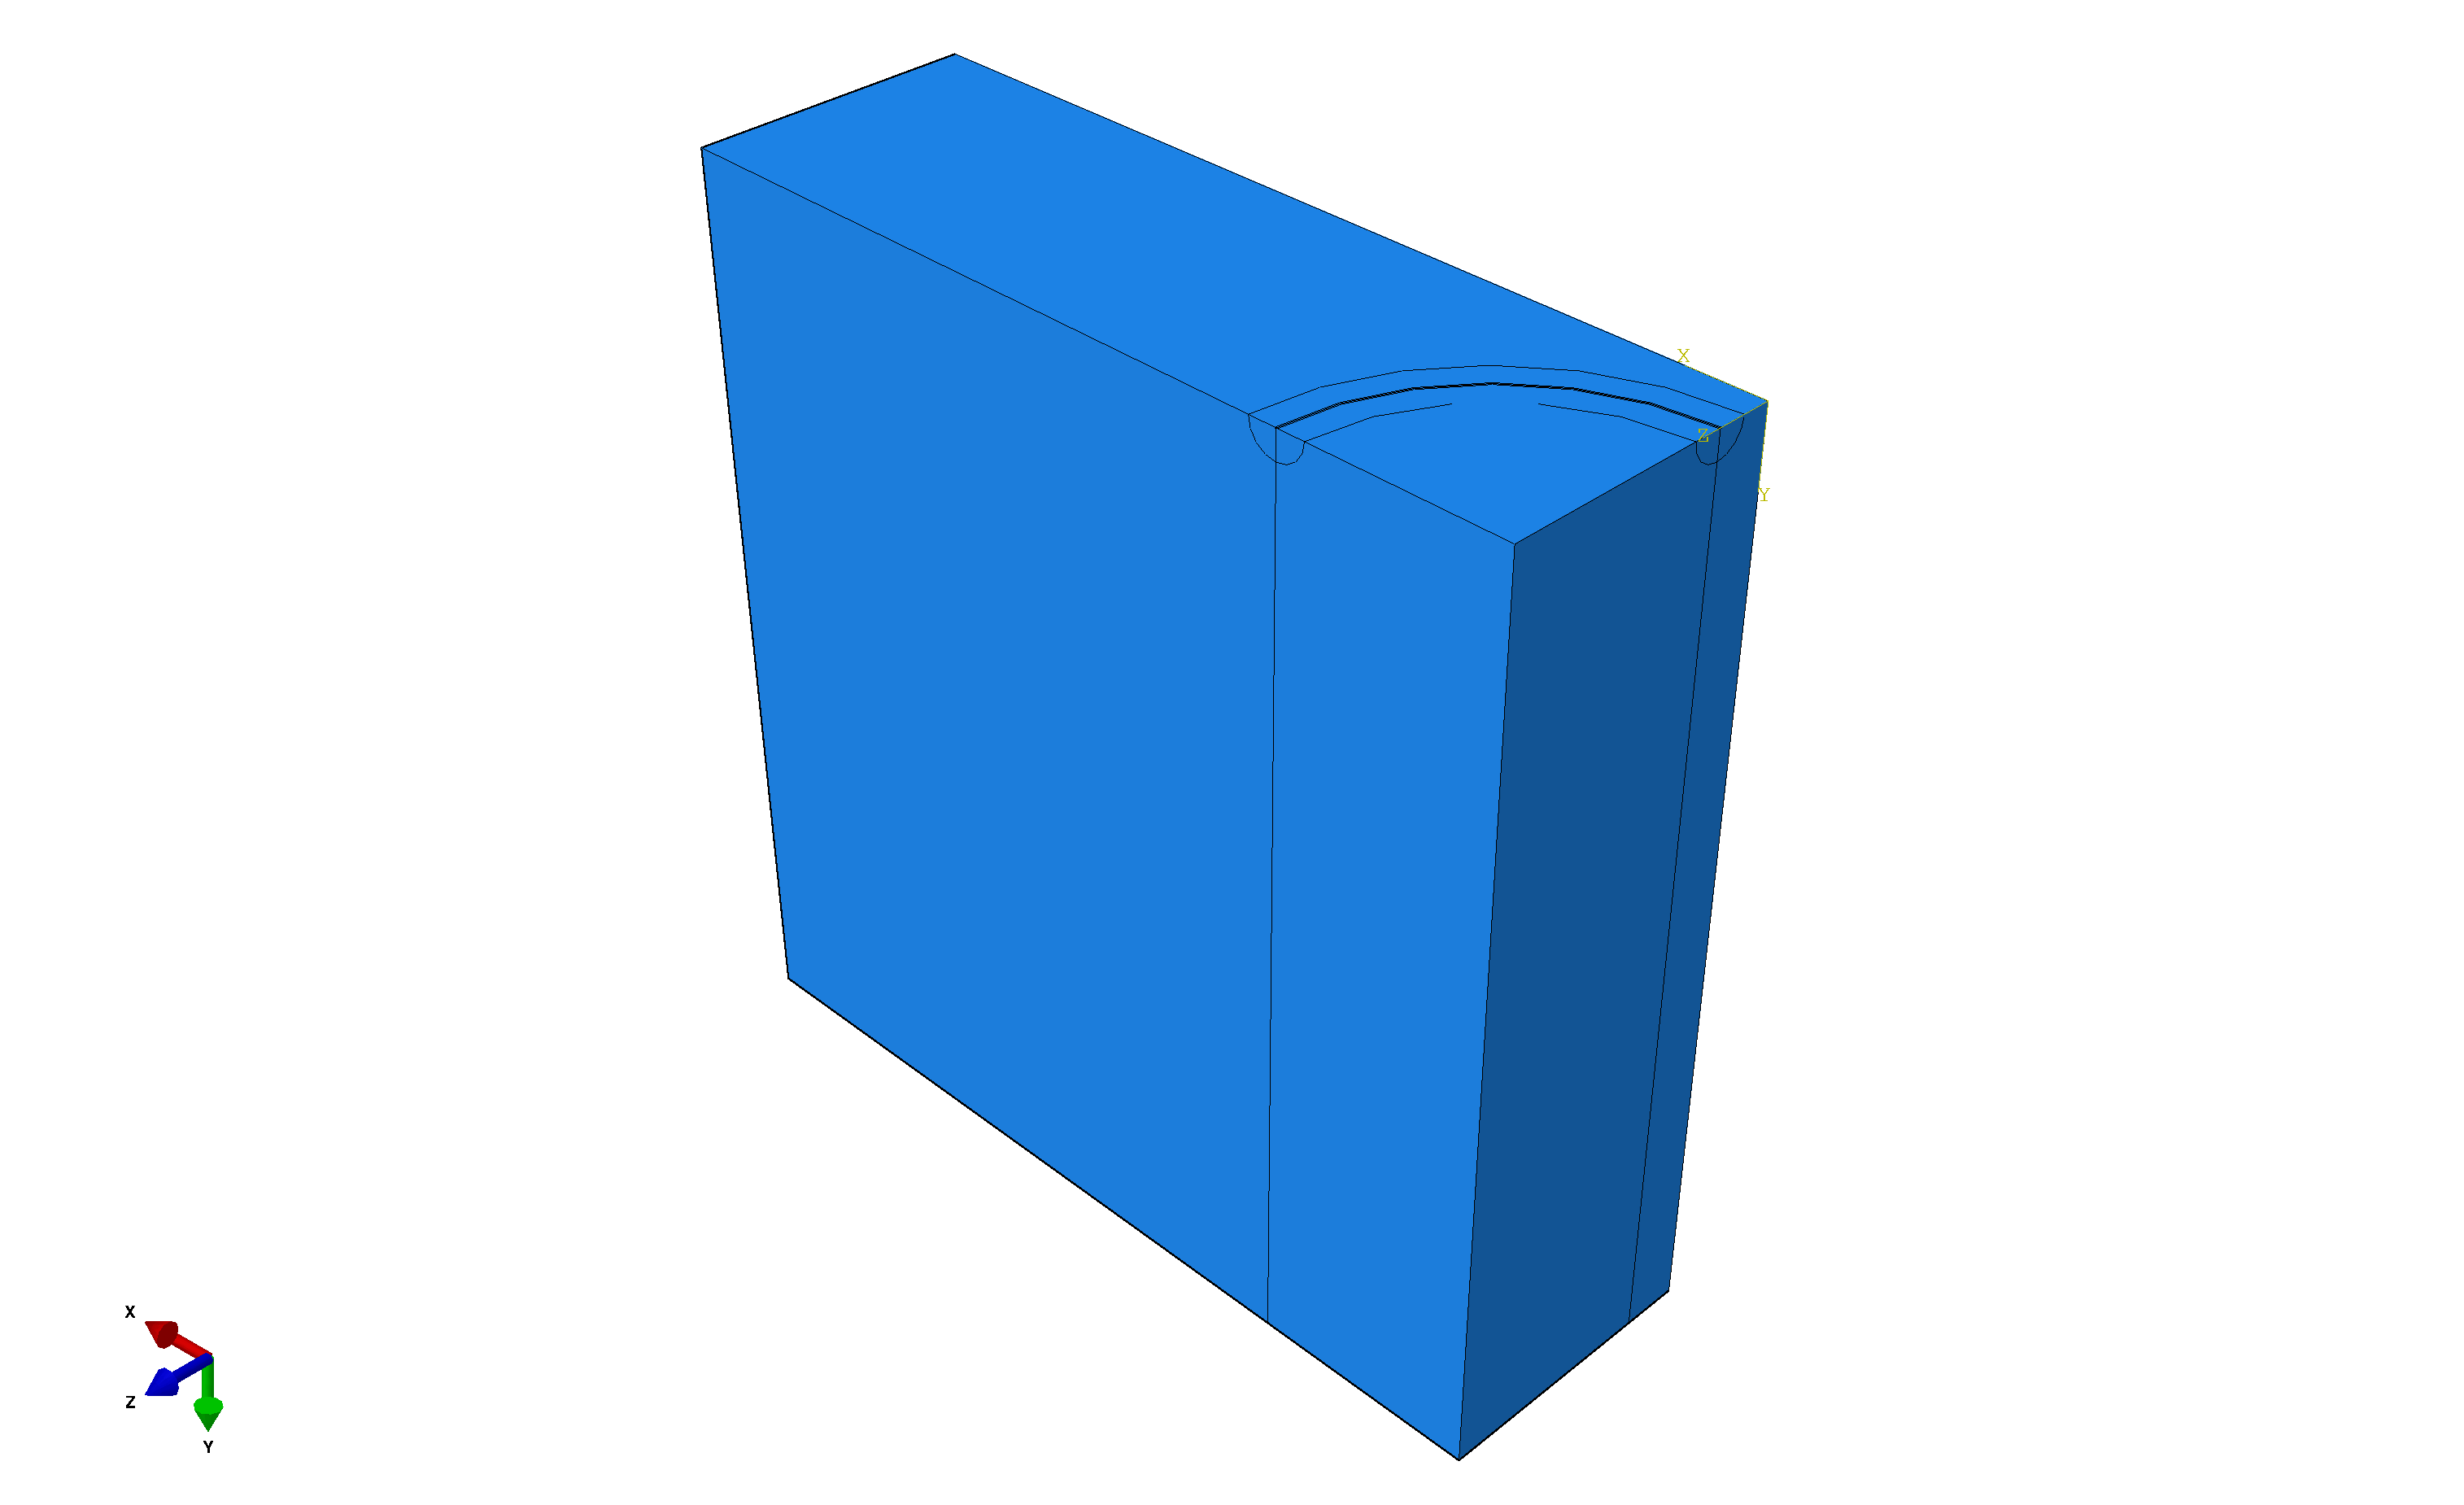
\includegraphics[width=\columnwidth]{model9-assembly}}
%    \mode<presentation>{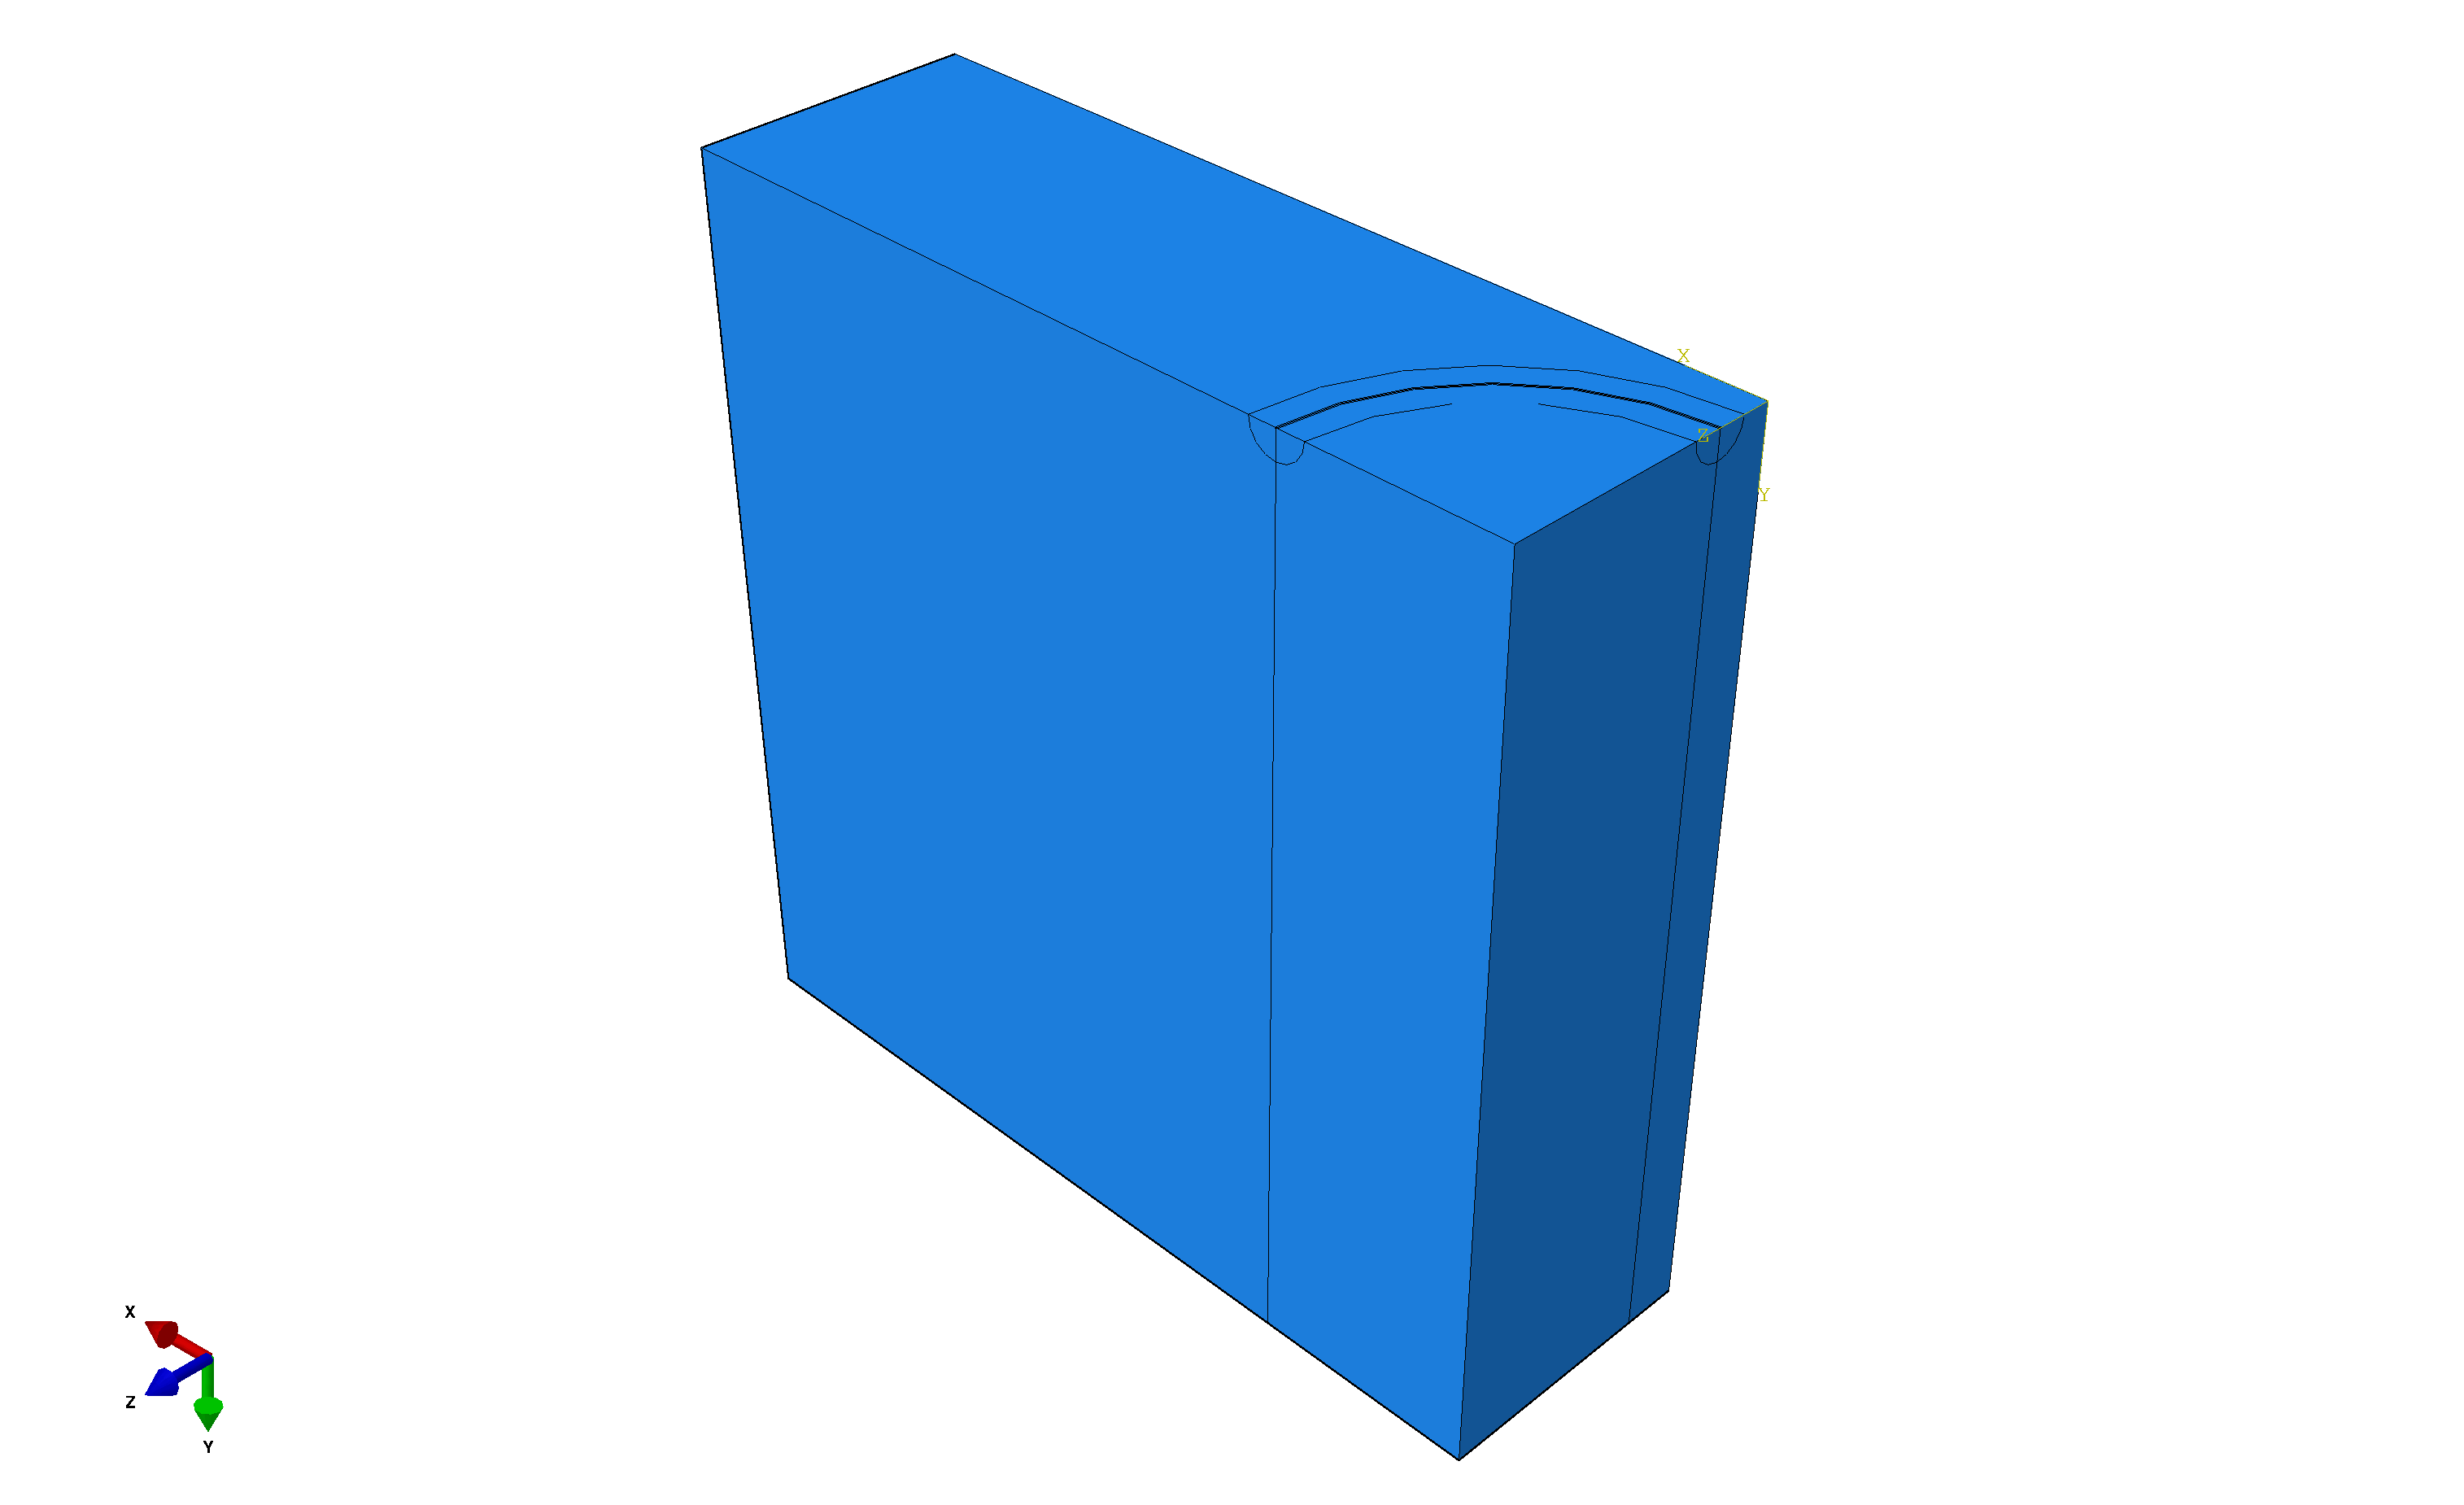
\includegraphics[width=0.7\columnwidth]{model9-assembly}}
%    \caption{McClung et al. model 9\label{fig:model9-assembly}}
%  \end{figure}
%\end{frame}
%\note{And this is Model 9, with a very deep, semi-circular crack front, generated from the same program.}
%
%\section{Further Updates to Quillen Abaqus Models}
%
Building from \citet{renfro2009}, the previously-described Python program created sets of models matching the plate and crack geometries given in \Cref{fig:geometries}.
For each of the nine geometries, finite element models with varying numbers of elements were created.
For each finite element mesh, one linear elastic and three Ramberg-Osgood elastic-plastic models were analyzed, and \J values were stored in the Abaqus ODB.
Finally, \hone values were calculated from the \J values to test for convergence and verification against earlier models.
A total of 144 models were analyzed, including 36 elastic models (nine geometries by four mesh densities) and 108 elastic-plastic models (nine geometries by four mesh densities by three Ramberg-Osgood hardening exponents).
Solving all the models required approximately 43 hours on one quad-core AMD Opteron compute cluster node, and created \SI{103}{\giga\byte} of output data. Extracting \hone data from the ODB files took only 7 minutes.
Mesh convergence for one model is shown in \Cref{fig:mesh-convergence}, and convergence on the ratio of \Jpl:\Jel is shown in \Cref{fig:j-convergence}.
Note that the mesh convergence is not due simply to creating smaller elements along the crack front.
As shown in \Cref{fig:model1-3-meshes}, the number of elements along the crack front only increases from 21 to 25.
Adding additional elements outside the crack region has an effect on the \J and \hone values calculated, indicating that this model set needs further development.
However, all three anomalous \hone results in \citet{quillen2005} have been eliminated, as shown in \Cref{fig:model1}.
The root cause of the anomalies (errors in the original files generated by FEACrack, possible unrecorded modifications to the files, bugs corrected in Abaqus, etc.) is still unknown.
\begin{frame}
\mode<presentation>{\begin{columns}[b]\begin{column}{0.45\textwidth}}
  \begin{figure}
    \centering
    \mode<article>{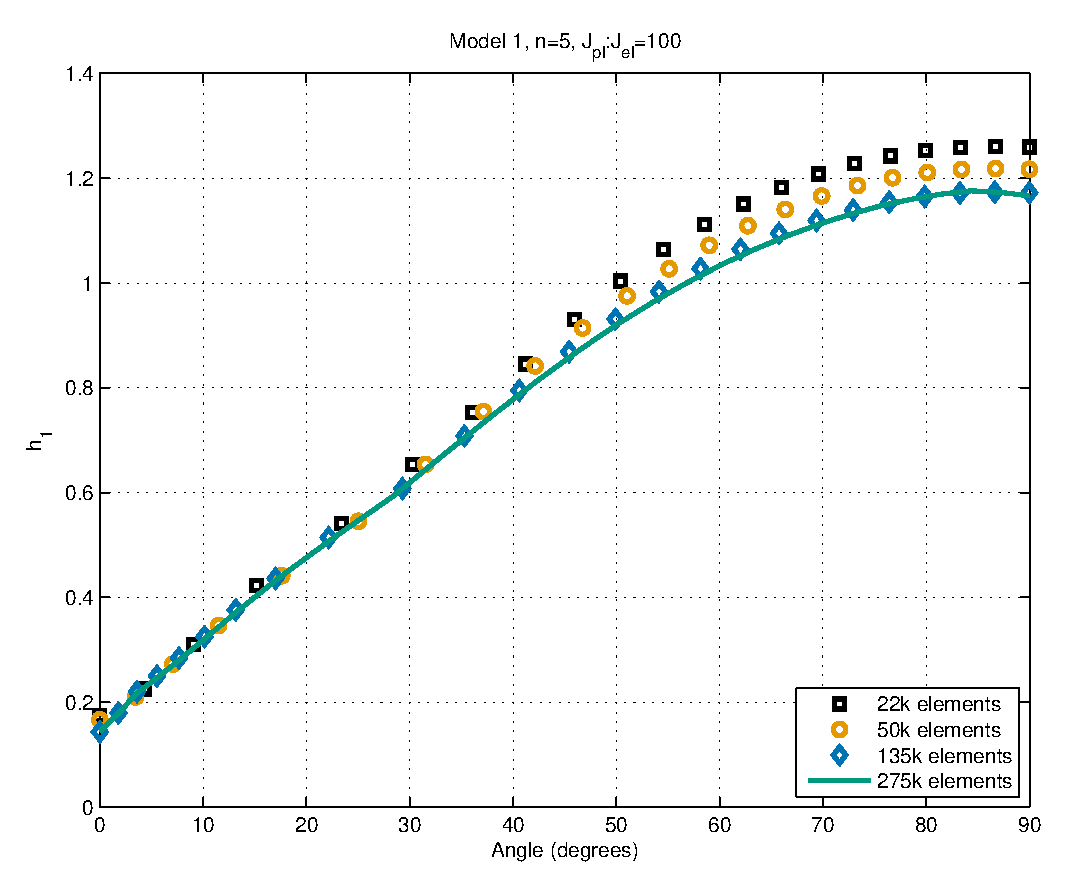
\includegraphics[width=0.5\columnwidth]{model1_n5_mesh_convergence}}
    \mode<presentation>{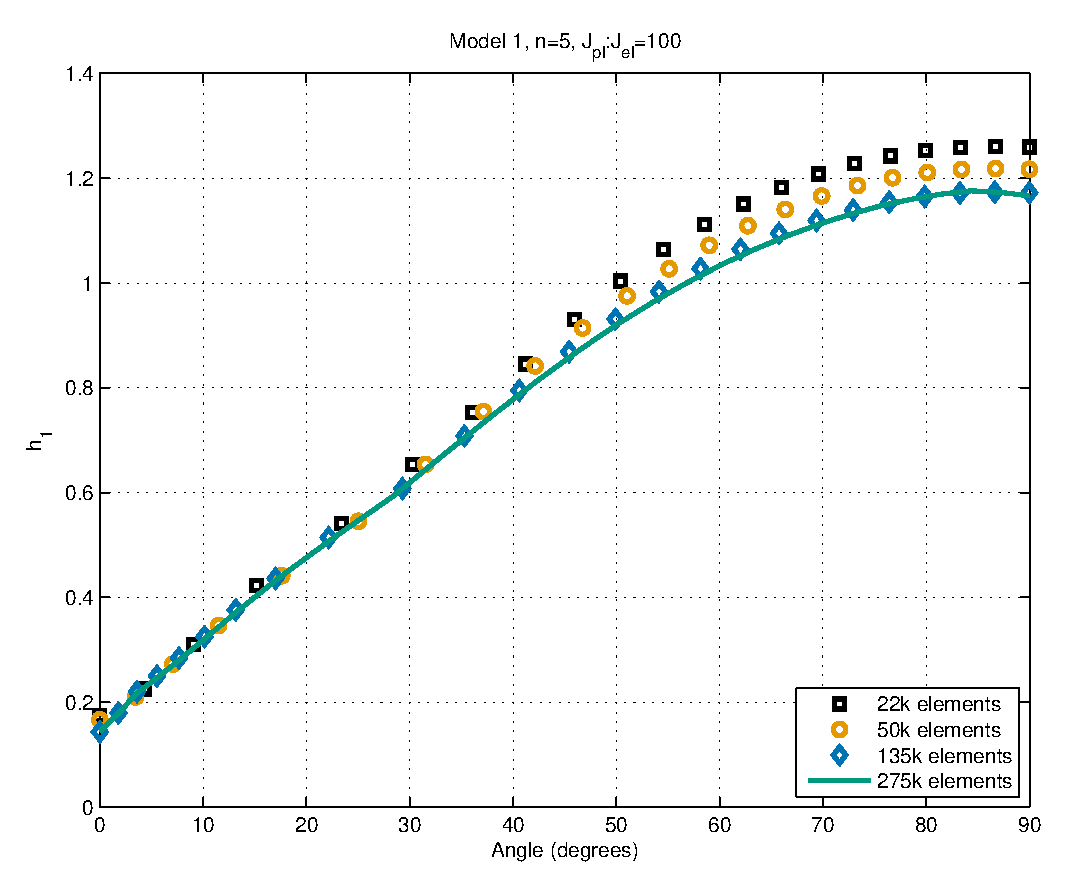
\includegraphics[width=\columnwidth]{model1_n5_mesh_convergence}}
    \caption{McClung et al. model 1 mesh convergence\label{fig:mesh-convergence}}
  \end{figure}
  \mode<presentation>{\end{column}\begin{column}{0.45\textwidth}}
%\end{frame}
%\begin{frame}
  \begin{figure}
    \centering
    \mode<article>{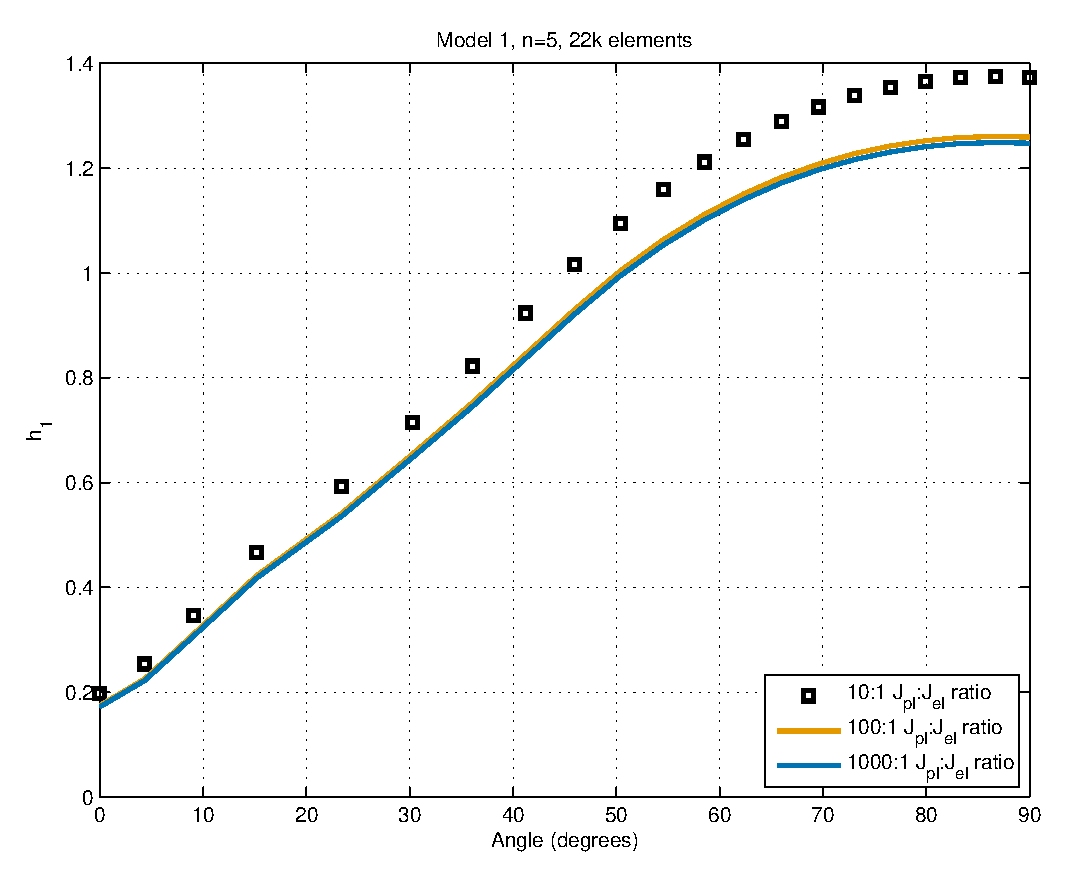
\includegraphics[width=0.5\columnwidth]{model1_n5_J_convergence}}
    \mode<presentation>{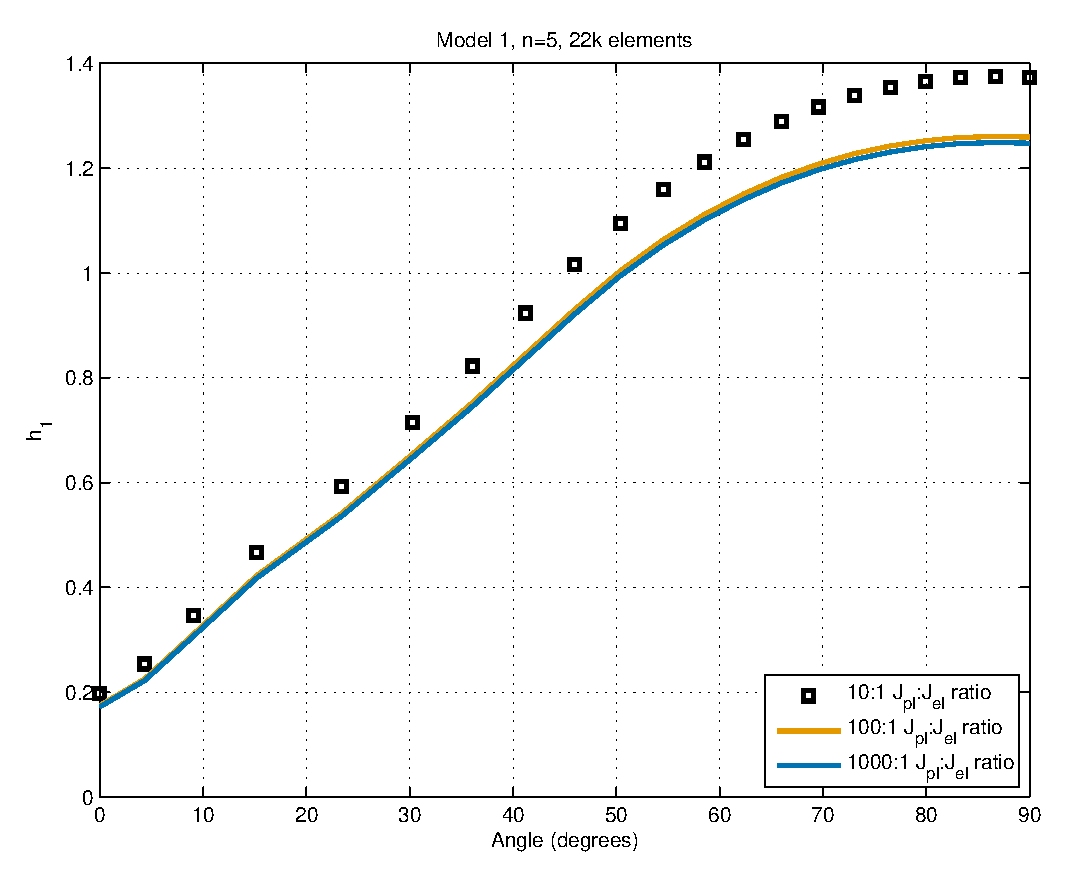
\includegraphics[width=\columnwidth]{model1_n5_J_convergence}}
    \caption{McClung et al. model 1 \J ratio convergence\label{fig:j-convergence}}
  \end{figure}
    \mode<presentation>{\end{column}\end{columns}}
\end{frame} \note{Two convergence studies were done on Model 1.

\vfill

One was to determine the influence of mesh density on \J results.

\vfill

The other was to determine the how much plastic deformation was required to give converged \J values.

\vfill

By default, when Abaqus is doing a fully plastic analysis for \J, is applies load until the ratio of \Jpl to \Jel is 10:1.

\vfill

But moving from a 10:1 ratio to a 100:1 ratio yielded substantial \J and \hone differences deep in the crack.

\vfill

The 100:1 and 1000:1 ratios returned virtually identical results.

\vfill
}
\begin{frame}
\mode<presentation>{\begin{columns}[t]\begin{column}{0.45\textwidth}}
  \begin{figure}
    \centering
    \mode<article>{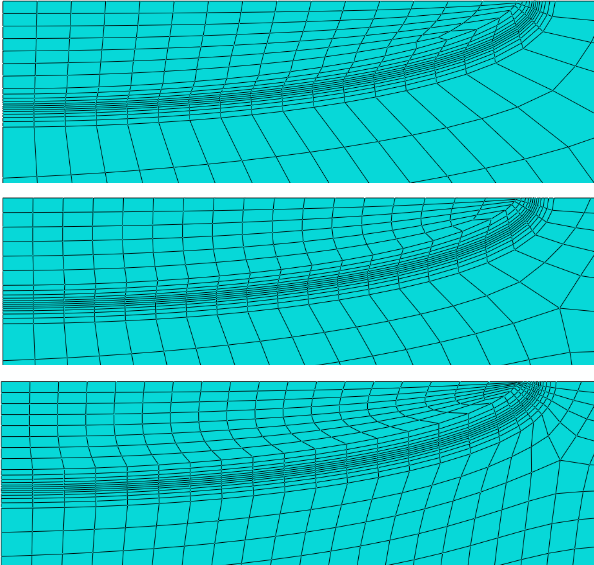
\includegraphics[width=0.5\columnwidth]{model1-3-meshes}}
    \mode<presentation>{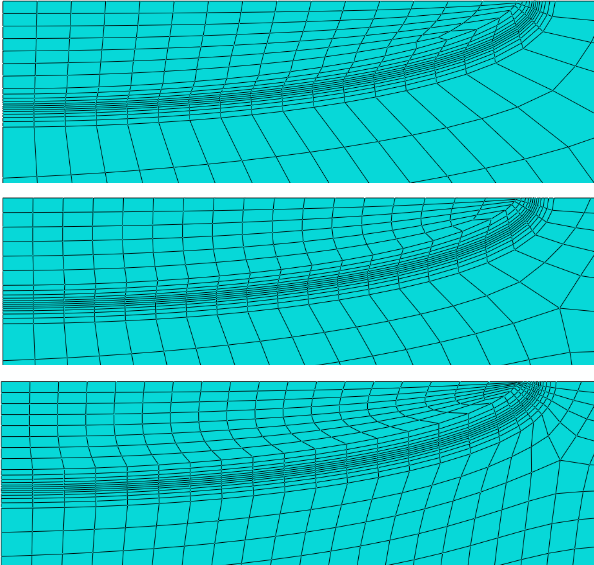
\includegraphics[width=0.8\columnwidth]{model1-3-meshes}}
    \caption{McClung et al. model 1 crack front mesh detail\label{fig:model1-3-meshes}}
  \end{figure}
  \mode<presentation>{\end{column}\begin{column}{0.45\textwidth}}
%\end{frame}
%
%\newcommand{\hfigure}[1]{
%\begin{figure} \centering \includegraphics[width=\hwidth]{h1_model#1}
%\caption{\hone comparison between McClung et al., Lei, Quillen, and Renfro, model #1 \label{fig:model#1}}
%\end{figure}
%}
%\newcommand{\hmissingfigure}[1]{
%\begin{figure} \centering \missingfigure[figwidth=\hwidth]{model #1}
%\caption{\hone comparison between McClung et al., Lei, Quillen, and Renfro, model #1 \label{fig:model#1}}
%\end{figure}
%}
%
%\begin{frame}
%  \mode<presentation>{
%    \frametitle{\hone comparisons among McClung et al., Lei, and Renfro, model 1}
%  }
  \begin{figure}
    \centering
    \mode<article>{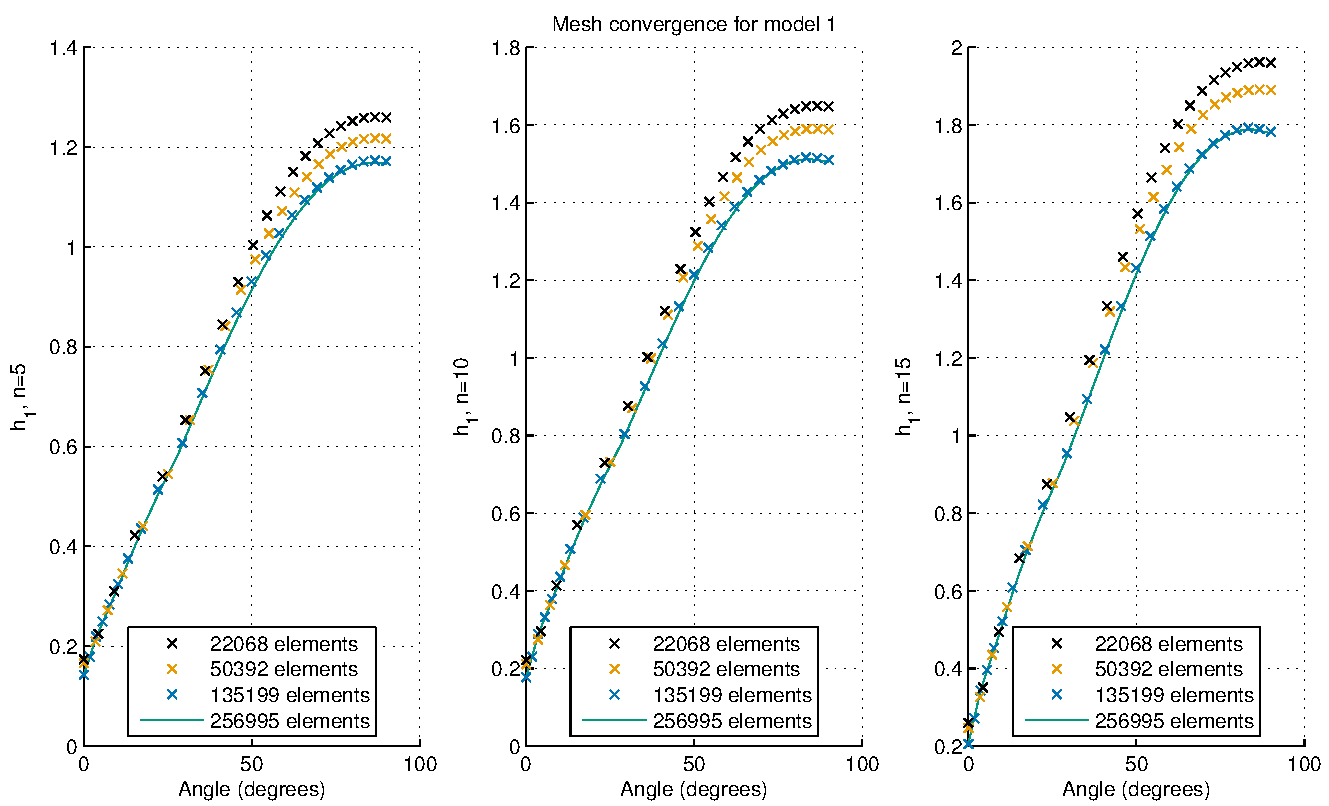
\includegraphics[width=0.8\columnwidth]{h1_model1}}
    \mode<presentation>{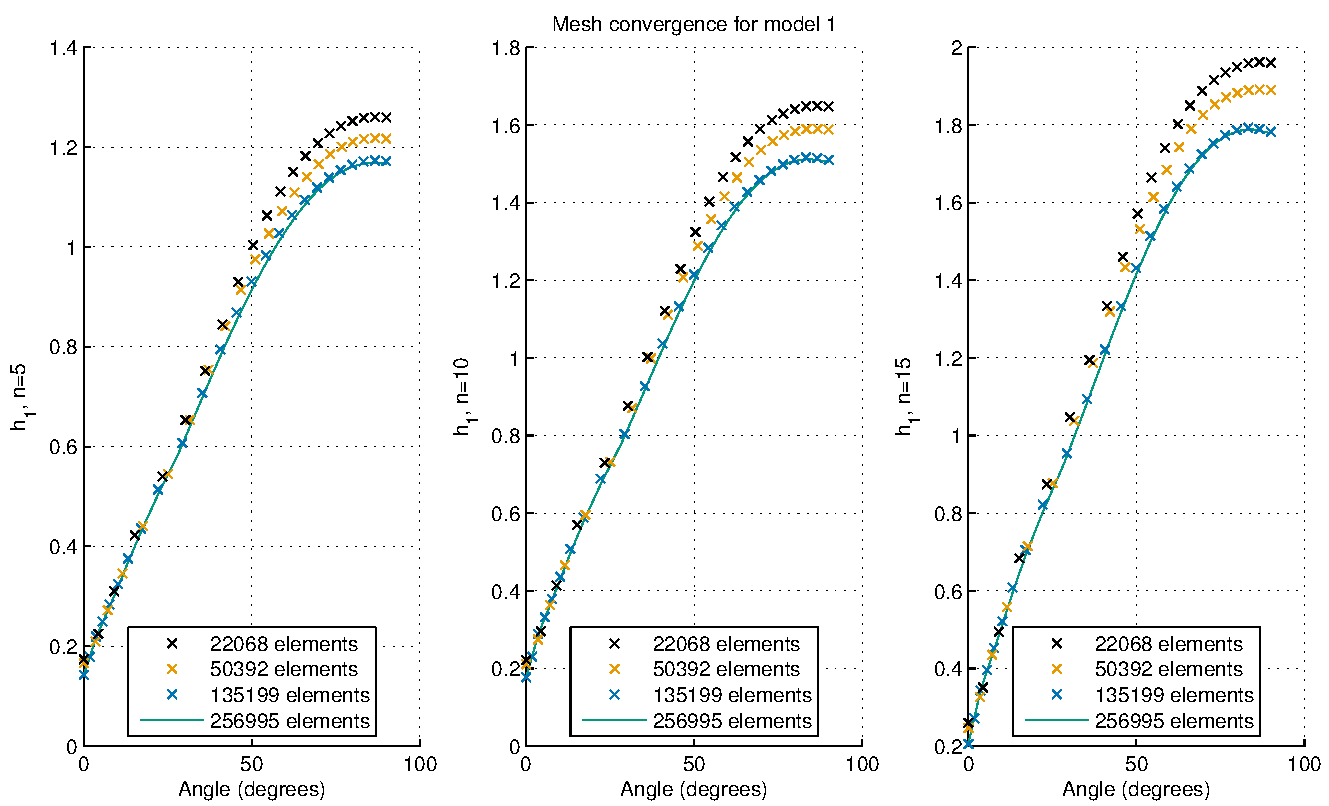
\includegraphics[width=\columnwidth]{h1_model1}}
    \mode<article>{\caption{\hone comparison between McClung et al., Lei, and Renfro, model 1 \label{fig:model1}}}
  \end{figure}
    \mode<presentation>{\end{column}\end{columns}}
\end{frame}
\note{Looking at the effect of the Ramberg-Osgood hardening exponent, it appears that harder materials (higher \(n\)) show more deviations from the McClung and Lei results than the softer material.}

\section{Verification of Two Tension Cases from Allen and Wells (2014)} \label{sec:verification-allen-wells}

\begin{frame}
%\mode<article>{Content that only goes in the dissertation}
\mode<presentation>{Content that only goes in the slides.}
\end{frame}
\note{A set of notes.

\vfill

Split the notes by sentence.

\vfill

Leaves plenty of room between them for referring to while presenting.

\vfill
}

This section will show the development of an improved set of modeling tools to study surface cracks in flat plates, using FEACrack, Python, and WARP3D.
These tools were first used to verify two tension models from \citeauthor{allenwells2014} (\citeyear{allenwells2014}), and then to solve an intermediate case, demonstrating the limits of the interpolation methodology.
Details of the algorithms used in the Python programs are given in \Crefrange{sec:preprocess}{sec:postprocess}.

\subsection{Identified Gaps in Interpolation Data}

\citeauthor{allenwells2014} built a set of 600 finite element models of surface cracks in tension, covering all combinations of
\begin{align*}
\frac{a}{t} &= 0.2, 0.4, 0.6, 0.8 & \frac{E}{\Sys} &= 100, 200, 300, 500, 700, 1000 \\
\frac{a}{c} &= 0.2, 0.4, 0.6, 0.8, 1.0 & n &= 3, 4, 6, 10, 20.
\end{align*}
Results for a set of models with \(\frac{a}{t}=0.6\) and \(n=6\) are shown in \Cref{fig:aspect-ratio-gap,fig:modulus-gap}.
The first figure shows a large gap between the results for cases \(\frac{a}{c}=0.2\) and \(\frac{a}{c}=0.4\), and the second figure shows a similar gap between the results for cases \(\frac{E}{\Sys}=100\) and \(\frac{E}{\Sys}=200\).
In each figure, normalized CMOD values for the more extreme case nearly double at comparable normalized stress levels, and the normalized \J values for the more extreme case are reduced by almost half at identical normalized CMOD levels.
As the authors use the solved models in a linear interpolation method, they identified a potential need for additional models with \(\frac{a}{c}=0.3\) and \(\frac{E}{\Sys}=150\), since there is no guarantee that the cracked plates exhibit linear behavior over such a wide range of results.
\begin{frame}
\begin{figure}[tbp]
%\forceversofloat
\centering
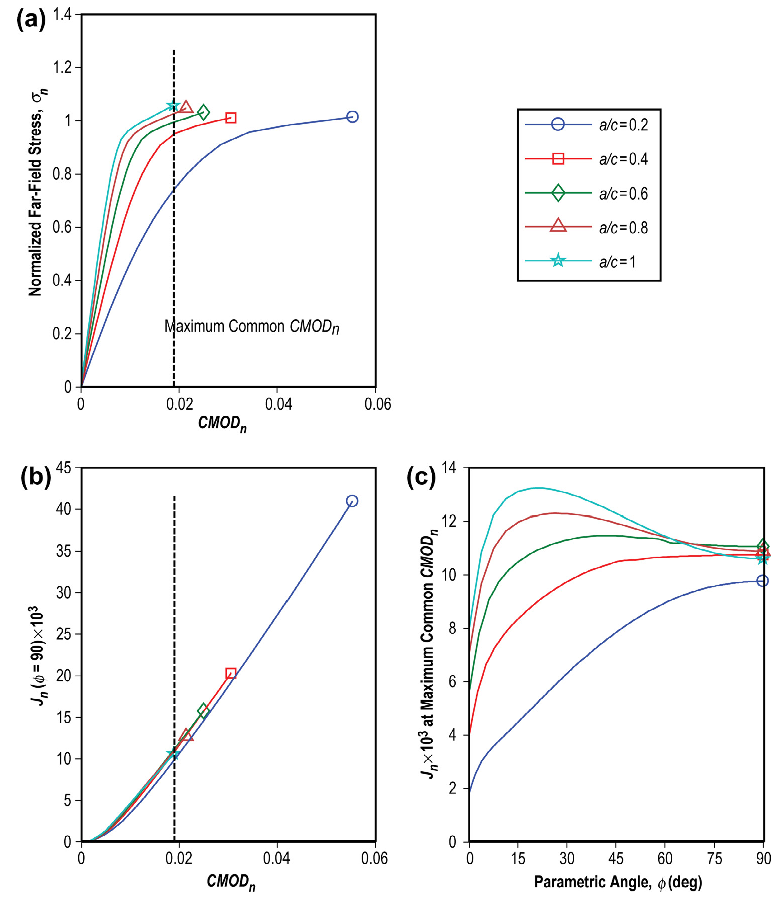
\includegraphics[width=0.7\columnwidth]{aspect-ratio-gap}
\caption{\label{fig:aspect-ratio-gap} Gap in results for very wide aspect ratios \citep{allenwells2014}}
\end{figure}
\begin{figure}[tbp]
\centering
%\forcerectofloat
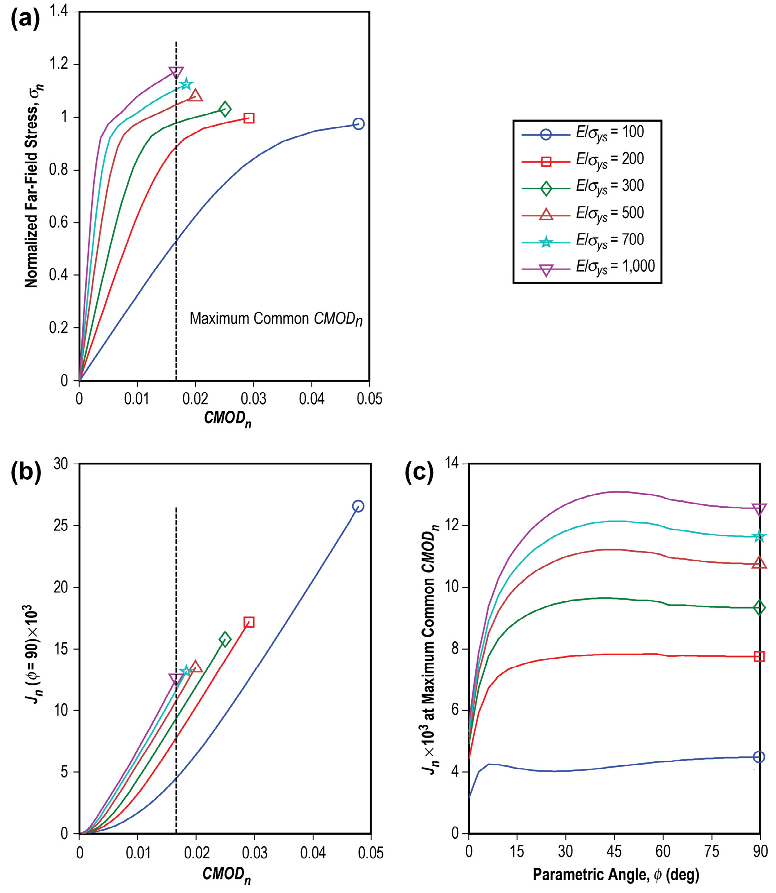
\includegraphics[width=0.7\columnwidth]{modulus-gap}
\caption{\label{fig:modulus-gap} Gap in results for very low elastic modulus values \citep{allenwells2014}}
\end{figure}
\end{frame}

\Cref{chap:app-verification-allen-wells} details the use of FEACrack \citep{feacrack} and WARP3D \citep{warp3d} to replicate the published results for the cases
\begin{align*}
\frac{a}{t} &= 0.6 & \frac{E}{\Sys} &= 100 \text{ and } 200\\
\frac{a}{c} &= 0.6 & n &= 6
\end{align*}
and the remainder of this chapter will show the results of a purpose-built model for \(\frac{E}{\Sys} = 150\) compared to an interpolated model using results from \(\frac{E}{\Sys}=100\) and \(\frac{E}{\Sys}=200\).

\subsection{Applying Procedure to New Material Model (\(\frac{E}{\Sys} = 150\))}

After modifying the \(\frac{E}{\Sys} = 200\) model from \Cref{chap:app-verification-allen-wells} to use \(E = 150\) and leaving the remote displacement at 0.0550, the new material model was solved.
As seen in \Cref{fig:e150_1}, the remote displacement was not high enough to place the model into the plastic regime, so the remote displacement was increased to 0.080.
The result of the new displacement is shown in \Cref{fig:e150_2}, and has clearly reached the plastic regime.
Later models used the secant method, and reached a CMOD of roughly 0.03.
\begin{frame}
\begin{figure}[tbp]
\centering
%\forcerectofloat
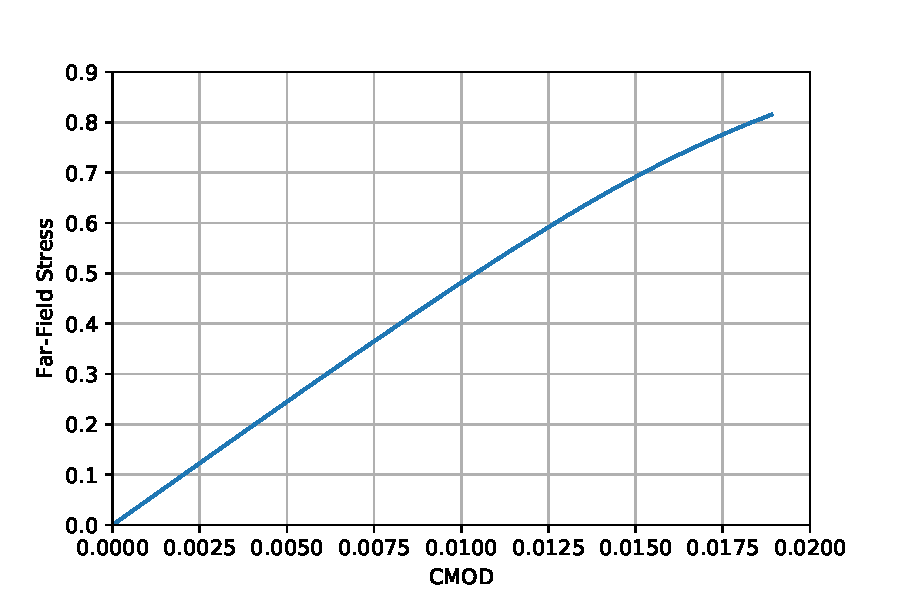
\includegraphics[width=0.8\columnwidth]{e150_1}
\caption{\label{fig:e150_1} First attempt at new material model}
\end{figure}
\end{frame}
\begin{frame}
\begin{figure}[tbp]
\centering
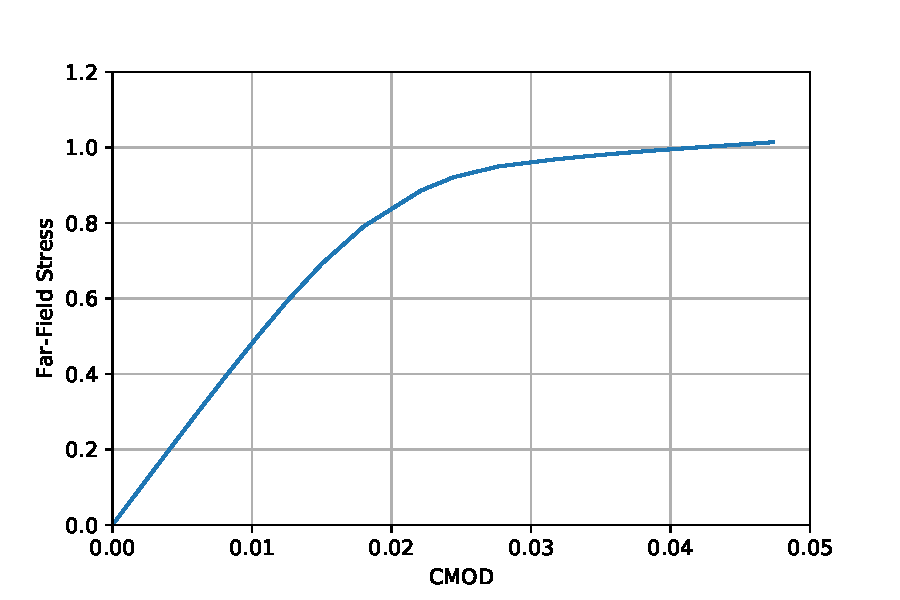
\includegraphics[width=0.8\columnwidth]{e150_2}
\caption{\label{fig:e150_2} Second attempt at new material model}
\end{figure}
\end{frame}

Finally, by comparing the \(\frac{E}{\Sys} = 150\) FEA results to the interpolated TASC result from \Cref{fig:tasc_interp_outputs}, we see that the FEA results are slightly more compliant in the elastic regime, and a sharper transition to the plastic regime at higher stress levels.
The two results differ by 5\% or less, as shown in \Cref{fig:e100_150_200_verification}.
\begin{frame}
\begin{figure}[tbp]
\centering
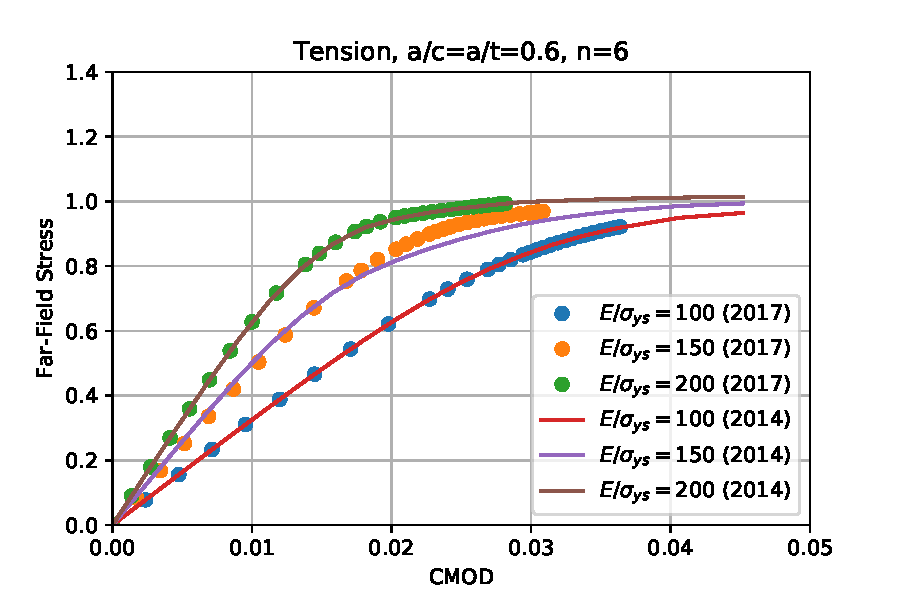
\includegraphics[width=0.8\columnwidth]{e100_150_200_verification}
\caption{\label{fig:e100_150_200_verification} Comparison of FEA result, interpolated result, and TASC raw data}
\end{figure}
\end{frame}

\subsection{Plotting CMOD, \J and \(\phi\)}

The final data to extract from the FEA results are values for the \J integral at each load increment. \J is a function of both load and position along the crack front, measured by the angle \(\phi\) from the free surface of the plate. \Cref{fig:j-phi-cmod-paa} shows an example of that function from \cite{allenwells2014}, and \Cref{fig:j-phi-cmod-mwr} shows a comparable function from the current models.

\begin{frame}
\begin{figure}[tbp]
\centering
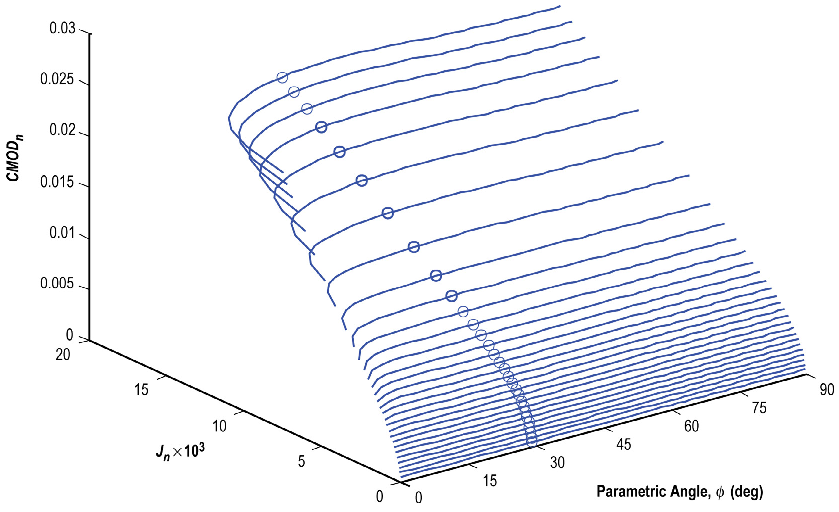
\includegraphics[width=0.8\columnwidth]{j-phi-cmod-paa}
\caption{\label{fig:j-phi-cmod-paa} Example relationship between \(\J(\phi)\) and CMOD \citep{allenwells2014}}
\end{figure}
\end{frame}

\begin{frame}
\begin{figure}[tbp]
\centering
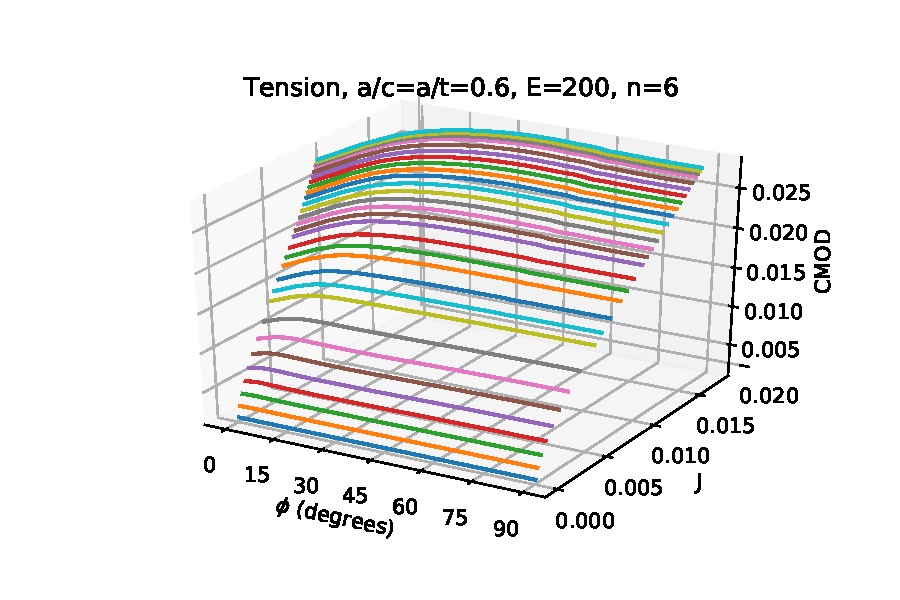
\includegraphics[width=0.8\columnwidth]{j-phi-cmod-mwr}
\caption{\label{fig:j-phi-cmod-mwr} Example relationship between \(\J(\phi)\) and CMOD}
\end{figure}
\end{frame}

%\begin{frame}[allowframebreaks]\mode<presentation>{\tiny}
%  \bibliography{cse_bibliography,v2}
%  \bibliographystyle{proposal}
%\end{frame}


In \Cref{sec:verification-allen-wells}, selected results from \cite{allenwells2014} were reproduced, and initial programs were developed to improve the rate at which new models can be created, solved, and results analyzed.
This also reduced the likelihood of manual error, and provided easier tracking of model changes.
%\J values have been extracted from the WARP3D output, and plotted against CMOD and angle from the free surface.
%Other values of \(E/\Sys\) may be needed for better interpolation, as there is a considerably larger gap in results between \(E/\Sys=100\) and \(E/\Sys=150\) than between \(E/\Sys=150\) and \(E/\Sys=200\).
The programs developed for verifying tension cases were generalized to bending cases, and the algorithms and structure of those programs is detailed below.

\section{Creating Plate Models}
\label{sec:preprocess}

All the surface crack models analyzed are similar in a parametric sense: each is a rectangular block of material with symmetric geometry and boundary conditions across the \(x\) and \(z\) axes.
Each surface crack has a semi-elliptical profile in the \(xy\) plane centered at the origin.
Since the bending models will be subjected to much larger displacements than tension models, the generic FEACrack model used for all geometries and materials is set to use a non-linear kinematic finite-strain element formulation supporting large rotations.
%\todo{Need to call out change from linear kinematic infinitesimal-strain element formulation to non-linear kinematic large-rotation finite-strain element formulation.}
Each plate subjected to bending loads is in 4-point bending with loads and supports acting in the \(y\) direction, and each plate subjected to tensile loads is loaded in the \(z\) direction.
Additionally, each plate analyzed should minimize finite width effects and ensure the crack face is in a state of pure bending.
Thus, for a plate of thickness \(t\) and crack size defined by \(\frac{a}{c}\) and \(\frac{a}{t}\),
\begin{align*}
W &= 5 \max{(c, t)} \\
S_\text{inner} &= W \\
S_\text{outer} &= 2W \\
L &= \max{(1.1 (S_\text{outer}), 2W)}
\end{align*}
where \(S_\text{inner}\) and \(S_\text{outer}\) are only defined for plates in bending.
Two example plates are shown in \Cref{fig:bend_ac02_at08_E0100_n03,fig:bend_ac10_at02_E0100_n03}, where each plate occupies extreme positions in terms of the crack geometry (and the plate width and length which are functions of crack width).
\begin{figure}[tbp]
\centering
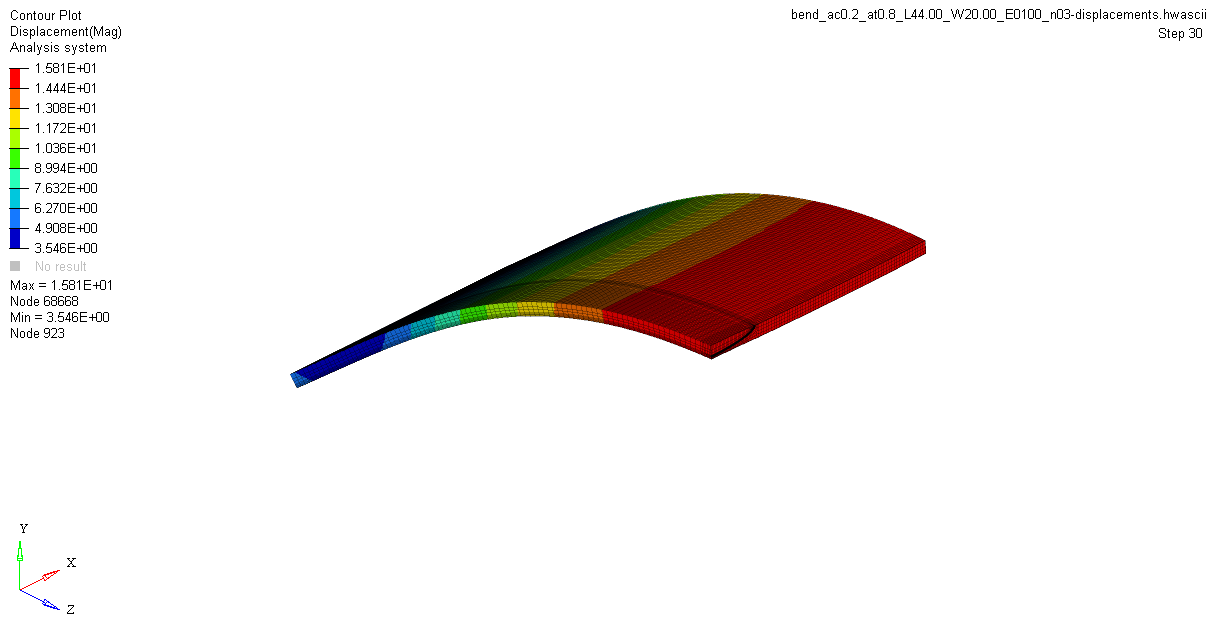
\includegraphics[width=\textwidth]{bend_ac02_at08_E0100_n03}
\caption{\label{fig:bend_ac02_at08_E0100_n03} Plate model, \(\frac{a}{c}=0.2\), \(\frac{a}{t}=0.8\)}
\end{figure}
\begin{figure}[tbp]
\centering
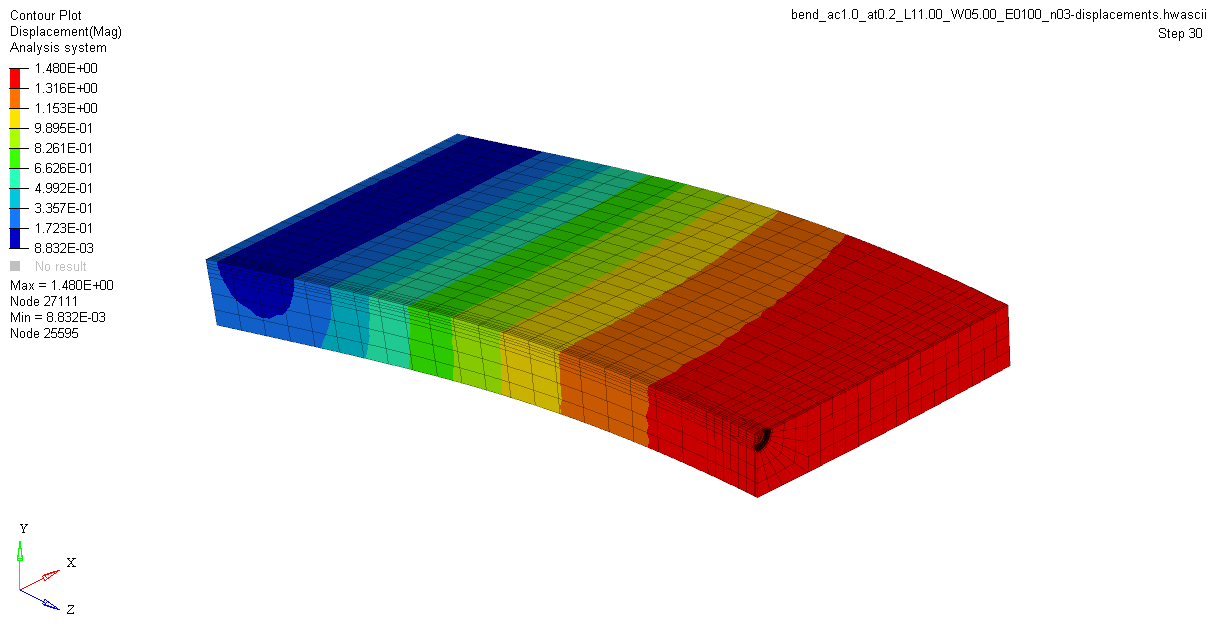
\includegraphics[width=\textwidth]{bend_ac10_at02_E0100_n03}
\caption{\label{fig:bend_ac10_at02_E0100_n03} Plate model, \(\frac{a}{c}=1.0\), \(\frac{a}{t}=0.2\)}
\end{figure}

After the geometry and mesh for a given cracked plate have been defined, the elastic modulus \(E\) and the plastic stress-strain curve must be defined.
Finally, each combination of plate geometry, mesh, and material properties must be written into separate WARP3D input files for analysis.
An algorithm for constructing these input files is given in \Cref{alg:plate-creator}, and a Python version of the algorithm for a subset of the problem space is given in \Cref{lst:plate-creator,lst:bend-config}.
The \verb|numpy| numeric Python libraries \cite{numpy} are used throughout the plate creation process to simplify any array-based operations. 
\begin{algorithm}[tbp]
  \caption{Plate Creator}
  \label{alg:plate-creator}
  \begin{algorithmic}
    \Procedure{Plate Creator}{} \Comment{Create a series of WARP3D input files}
    \State Read lists of $\frac{a}{t}$, $\frac{a}{c}$, $\frac{E}{\sigma_{\text{ys}}}$, $n$ values from configuration
    \State \Comment{typically: $0.2 \leq \frac{a}{t} \leq 0.8$, $0.2 \leq \frac{a}{c} \leq 1.0$, $100 \leq \frac{E}{\sigma_\text{ys}} \leq 1000$, $3 \leq n \leq 20$}
    \State Read $t$, $\sigma_\text{ys}$, global .elt file from configuration
    \State \Comment{typically: $t=1$, $\sigma_\text{ys}=1$, and global .elt file = 'bend.elt'}
    \ForAll{($\frac{a}{t}$ values, $\frac{a}{c}$ values)}
      \State $(a, c, L, W, S_{\text{in}}, S_{\text{out}}) \gets \Call{Set Geometry}{\text{global .elt file}, \frac{a}{c}, \frac{a}{t}, t}$
      \State $\text{generic mesh} \gets \Call{Build Mesh}{\text{global .elt file}, a, c, t, L, W, S_{\text{in}}, S_{\text{out}}}$
      \State \Comment{creates an input file with an arbitrary material for every combination of $\frac{a}{c}$ and $\frac{a}{t}$}
      \ForAll{($\frac{E}{\sigma_\text{ys}}$ values, $n$ values)}
        \State $E \gets (\frac{E}{\sigma_\text{ys}})(\sigma_\text{ys})$
        \State $\text{WARP3D input} \gets \Call{Set Material}{\text{generic mesh}, E, \sigma_\text{ys}, n}$
        \State \Comment{creates an input file for every combination of $\frac{a}{c}$, $\frac{a}{t}$, $E$, and $n$}
      \EndFor
    \EndFor
    \EndProcedure
  \end{algorithmic}
\end{algorithm}

\begin{Spacing}{1}
\begin{lstlisting}[language=Python,caption={Python implementation of Plate Creator algorithm}, label=lst:plate-creator]
# plate_creator.py
import preprocess as pre
from bend_config import aspect_ratio_list, depth_ratio_list
from bend_config import plate_thickness, E_Sys_ratio_list
from bend_config import Sys, n_list
from bend_config import elt_global_template_filename

for depth_ratio in depth_ratio_list:
    for aspect_ratio in aspect_ratio_list:
        (a, c, W, t, L,
         S_inner, S_outer) = pre.calculate_geometry(
                     elt_global_template_filename,
                     depth_ratio, aspect_ratio,
                     plate_thickness)
        geom_filename = pre.build_mesh(
                elt_global_template_filename, a, c, L, W, t,
                S_inner, S_outer)
        print("Wrote generic mesh {0}".format(geom_filename))
        for n in n_list:
            for E_Sys_ratio in E_Sys_ratio_list:
                E = Sys*E_Sys_ratio
                model_filename = pre.change_material_properties(
                        inp_filename=geom_filename,
                        E=E, Sys=Sys, n=n)
                print("Wrote {0}".format(model_filename))
\end{lstlisting}
\end{Spacing}

\begin{Spacing}{1}
\begin{lstlisting}[language=Python,caption={Python implementation for subset of geometry and material configurations}, label=lst:bend-config]
# bend_config.py
aspect_ratio_list = [0.2, 0.4, ]
depth_ratio_list = [0.2, 0.4, 0.6, 0.8, ]
plate_thickness = 1.0
E_Sys_ratio_list = [100.0, 200.0, 300.0, 500.0, 700.0, 1000.0, ]
Sys = 1.0
n_list = [3, 4, 6, 10, 20, ]
elt_global_template_filename = 'bend.elt'
\end{lstlisting}
\end{Spacing}

The remaining algorithms will be shown only as pseudocode in order to emphasize the structure of the algorithms instead of their specific implementation.
Readers interested in the Python implementation can download a copy of the Python source files from \url{https://github.com/mikerenfro/NAMEOFREPO}\todo{Make a Github repo for the whole set of Python and supporting files.}

\subsection{Defining Plate Model Geometry}

\Cref{alg:set_geometry} uses \Cref{alg:get_type} to determine if the model is in bending or tension, and calculates the necessary plate dimensions from given values for crack aspect ratio, crack depth ratio, and plate thickness.
\Cref{alg:get_type} looks through an FEACrack input file for specific commands in the file's notes field and commands.
If a traction in the \(y\) direction is defined in the notes field, and two rigid roller surfaces are found in the model commands, the model is assumed to represent a plate in bending.
Otherwise, the model is assumed to represent a plate in tension.
\Cref{alg:build_mesh} uses \Cref{alg:get_elt_filename} to define the name of a new FEACrack input file, copies the generic FEACrack input file to the new name, uses \Cref{alg:adjust_roller_positions} to modify the roller locations if the input file represents a plate in bending, and runs FEACrack with command arguments to create a WARP3D input file with the correct plate geometry and crack size.
\Cref{alg:get_elt_filename} takes the name of the generic FEACrack input file and a list of dimension values, and defines a new FEACrack input filename with the dimension values included.
\Cref{alg:adjust_roller_positions} searches an FEACrack input file for commands representing the position of rollers, and changes their \(z\) dimensions to match \Sinner and \Souter.
\begin{algorithm}[tbp]
  \caption{Set Geometry}
  \label{alg:set_geometry}
  \begin{algorithmic}
    \Procedure{Set Geometry}{$\text{global .elt file}, \frac{a}{c}, \frac{a}{t}, t$} \Comment{Calculate plate dimensions}
    \State $a \gets (\frac{a}{t})t$
    \State $c \gets a (\frac{a}{c})^{-1}$
    \If{$c > t$}
      \State $W \gets 5c$
    \Else
      \State $W \gets 5t$
    \EndIf
    \State $\text{model type} \gets \Call{Get Type}{\text{global .elt file}}$
    \If{model type = 'bending'}
      \State $\Sinner \gets W$
      \State $\Souter \gets 2W$
      \If{$2 W > 1.1 \Souter$}
        \State $L \gets 2 W$
      \Else
        \State $L \gets 1.1 \Souter$
      \EndIf
    \Else
      \State $\Sinner \gets \text{Null}$
      \State $\Souter \gets \text{Null}$
      \State $L \gets 2 W$
    \EndIf
    \State \textbf{return} $(a, c, W, L, \Sinner, \Souter)$
    \EndProcedure
  \end{algorithmic}
\end{algorithm}

\begin{algorithm}[tbp]
  \caption{Get Type}
  \label{alg:get_type}
  \begin{algorithmic}
    \Procedure{Get Type}{global .elt file} \Comment{determine if a .elt file is for a bending or a tension model}
      \If{'"*use bottom load pin plate ty ' found in 'Notes:' field}
        \If{'RigidSurfaceData\_Radius' found twice}
          \If{'RigidSurfaceData\_PinLocation' found twice}
            \State model type $\gets$ 'bending'
          \Else
            \State model type $\gets$ 'invalid'
          \EndIf
        \EndIf
      \Else
        \State model type $\gets$ 'tension'
      \EndIf
      \State \textbf{return} model type
    \EndProcedure
  \end{algorithmic}
\end{algorithm}

\begin{algorithm}[tbp]
  \caption{Build Mesh}
  \label{alg:build_mesh}
  \begin{algorithmic}
    \Procedure{Build Mesh}{{global .elt file}, $a$, $c$, $t$, $L$, $W$, $\Sinner$, $\Souter$}
      \State \Comment{use FEACrack create a WARP3D input file with an arbitrary material}
      \State {model .elt file} $\gets$ \Call{Get Elt Filename}{{global .elt file}, $a$, $c$, $L$, $W$, $t$} 
      \State \Comment{'bend\_ac$(\frac{a}{c})$\_at$(\frac{a}{t})$\_L$(L)$\_W$(W)$.elt'}
      \State Copy {global .elt file} to {model .elt file}
      \If{$\Sinner \neq \text{Null} \AND \Souter \neq \text{Null}$}
        \State \Call{Adjust Roller Positions}{model .elt file, $\Sinner$, $\Souter$}
      \EndIf
      \State Run FEACrack program on model .elt file, using $a$, $2c$, $t$, $L$, and $W$
      \State \textbf{return} \text{generic mesh file} \Comment{'bend\_ac$(\frac{a}{c})$\_at$(\frac{a}{t})$\_L$(L)$\_W$(W)$\_wrp.inp'}
    \EndProcedure
  \end{algorithmic}
\end{algorithm}%\todo{Unify notation between \Sinner and \(S_{\text{in}}\), same with outer.}

\begin{algorithm}[tbp]
  \caption{Get Elt Filename}
  \label{alg:get_elt_filename}
  \begin{algorithmic}
    \Procedure{Get Elt Filename}{global .elt file, $a$, $c$, $L$, $W$, $t$}
      \State \Comment{determine the name of a .elt file for a given geometry}
      \State prefix $\gets$ global .elt file basename \Comment{'bend'}
      \State middle $\gets$ '\_ac$(\frac{a}{c})$\_at$(\frac{a}{t})$\_L$(L)$\_W$(W)$'
      \State suffix $\gets$ '.elt'
      \State \textbf{return} prefix + middle + suffix \Comment{'bend\_ac$(\frac{a}{c})$\_at$(\frac{a}{t})$\_L$(L)$\_W$(W)$.elt'}
    \EndProcedure
  \end{algorithmic}
\end{algorithm}

\begin{algorithm}[tbp]
  \caption{Adjust Roller Positions}
  \label{alg:adjust_roller_positions}
  \begin{algorithmic}
    \Procedure{Adjust Roller Positions}{model .elt file, $\Sinner$, $\Souter$}
    \State \Comment{move roller positions in .elt file to $\Sinner$ and $\Souter$}
    \If{first 'RigidSurfaceData\_PinLocation' found in model .elt file}
      \State Change $z$ value of location to $\Sinner$
    \EndIf
    \If{second 'RigidSurfaceData\_PinLocation' found in model .elt file}
      \State Change $z$ value of location to $\Souter$
    \EndIf
    \EndProcedure
  \end{algorithmic}
\end{algorithm}

\subsection{Defining Material Properties}

\Cref{alg:set_material} calls \Cref{alg:get_specific_model_filename} to determine the name of a WARP3D input file for a specific material, copies the WARP3D input file for the current geometry to the new name, and examines the new WARP3D input file for lines representing the plastic behavior of the material. Those lines are replaced with the results of \Cref{alg:lppl} for a given elastic modulus, yield strength, and hardening exponent.
\Cref{alg:get_specific_model_filename} takes the name of the WARP3D file for the current geometry and defines a new WARP3D input filename with the elastic modulus and hardening exponent values included.
\Cref{alg:lppl} defines a set of plastic strain values that are finely spaced near the onset of yield, and increasingly coarse as plastic strain increases, and uses a power law relationship to define the corresponding set of true stress values. This ensures a smooth transition from linear behavior without using an excessive total number of points on the curve.

\begin{algorithm}[tbp]
  \caption{Set Material}
  \label{alg:set_material}
  \begin{algorithmic}
    \Procedure{Set Material}{generic .inp file, $E$, $\sigma_\text{ys}$, $n$}
    \State \Comment{modify arbitrary material parameters in input file to specified values}
    \State specific .inp file $\gets$ \Call{Get Specific Model Filename}{generic .inp file, $E$, $\sigma_\text{ys}$, $n$}
    \State \Comment{'bend\_ac$(\frac{a}{c})$\_at$(\frac{a}{t})$\_L$(L)$\_W$(W)$\_E$(E)$\_n$(n)$\_wrp.inp'}
    \State Copy generic .inp file to specific .inp file
    \If{'stress-strain curve      1' found in specific .inp file}
      \State change stress-strain curve data to \Call{LPPL}{$E$, $\sigma_\text{ys}$, $n$}
    \EndIf
    \State change $E$ value in specific .inp file
    \State \textbf{return} specific .inp file \Comment{'bend\_ac$(\frac{a}{c})$\_at$(\frac{a}{t})$\_L$(L)$\_W$(W)$\_E$(E)$\_n$(n)$\_wrp.inp'}

    \EndProcedure
  \end{algorithmic}
\end{algorithm}

\begin{algorithm}[tbp]
  \caption{Get Specific Model Filename}
  \label{alg:get_specific_model_filename}
  \begin{algorithmic}
    \Procedure{Get Specific Model Filename}{.inp filename, $E$, $\sigma_\text{ys}$, $n$}
      \State \Comment{determine the name of a specific .inp file for a given geometry and material parameters}
      \State prefix $\gets$ .inp file basename \Comment{'bend\_ac$(\frac{a}{c})$\_at$(\frac{a}{t})$\_L$(L)$\_W$(W)$\_wrp'}
      \State prefix $\gets$ prefix without last 4 characters
      \State \Comment{'bend\_ac$(\frac{a}{c})$\_at$(\frac{a}{t})$\_L$(L)$\_W$(W)$'}
      \State middle $\gets$ '\_E$(E)$\_n$(n)$'
      \State suffix $\gets$ '\_wrp.inp'
      \State \textbf{return} prefix + middle + suffix
      \State \Comment{'bend\_ac$(\frac{a}{c})$\_at$(\frac{a}{t})$\_L$(L)$\_W$(W)$\_E$(E)$\_n$(n)$\_wrp.inp'}
    \EndProcedure
  \end{algorithmic}
\end{algorithm}

\begin{algorithm}[tbp]
  \caption{LPPL}
  \label{alg:lppl}
  \begin{algorithmic}
    \Procedure{LPPL}{$E$, $\sigma_\text{ys}$, $n$} \Comment{calculate the plastic stress-strain curve for a power law material}
    \State $\epsilon_{\text{pl1}} \gets (0.001, 0.002, \cdots , 0.008)$
    \State $\epsilon_{\text{pl2}} \gets (0.013, 0.018, 0.023, 0.028)$
    \State $\epsilon_{\text{pl3}} \gets (0.038, 0.048, \cdots , 0.108)$
    \State $\epsilon_{\text{ys}} \gets \frac{\sigma_\text{ys}}{E}$
    \State $\epsilon \gets \epsilon_{\text{ys}} + (\epsilon_{\text{pl1}}, \epsilon_{\text{pl2}}, \epsilon_{\text{pl3}})$
    \State $\sigma \gets \sigma_\text{ys}  (\frac{\epsilon}{\epsilon_{\text{ys}}})^{\frac{1}{n}}$
    \State \textbf{return} $\epsilon$, $\sigma$
    \EndProcedure
  \end{algorithmic}
\end{algorithm}

\section{Solving Plate Models, Optimizing Boundary Conditions}
\label{sec:solve}

Now that the plate geometry, material properties, and boundary conditions are defined for a set of models, a procedure for solving for reaction forces, \J values, and CMOD values must be developed.
The boundary conditions applied to the model must be large enough to exhibit substantial amounts of plastic deformation, but not so large as to cause the model to exceed its material limits or become numerically unstable.
In \cite{allenwells2014}, the models were reported to have been deformed enough to cause the deformation level
\begin{align}
M &= \frac{r_{\phi} \Sys}{\J}
\end{align}
to drop below 20 or 25, but upon examining the TASC database, approximately half the models had minimum \(M\) values over 25, and about 10\% of the models had \(M\) values over 50, as seen in \Cref{fig:min-M-hist}.
Regardless of the exact deformation required, all models in the TASC database must contain enough data to perform accurate linear extrapolations from the \(\sigma\)-CMOD and \J-CMOD curves, similar to the curves shown in \Cref{fig:J-CMOD-extrapolation}.

\begin{figure}[tbp]
\centering
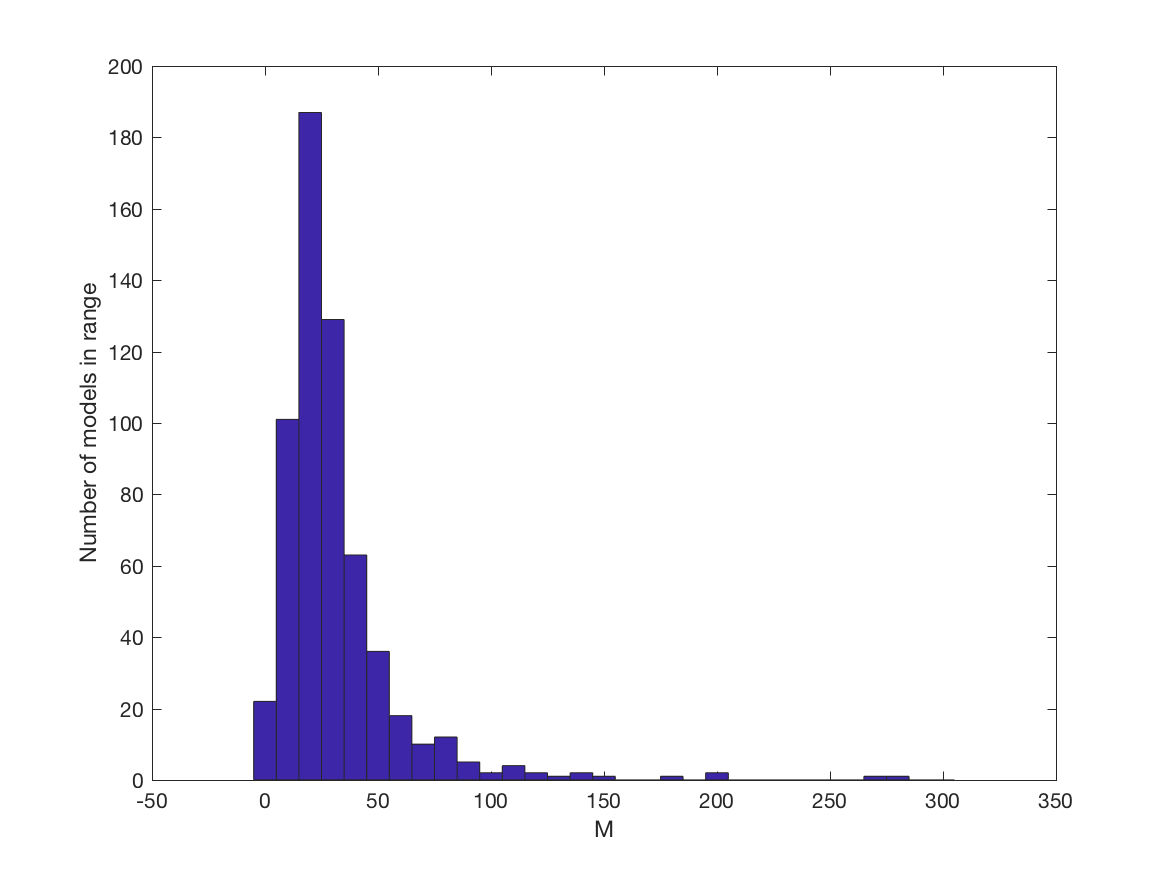
\includegraphics[width=0.7\columnwidth]{min_M_hist}
\caption{\label{fig:min-M-hist} Histogram of \(M\) results from TASC tension model database}
\end{figure}

\begin{figure}[tbp]
\centering
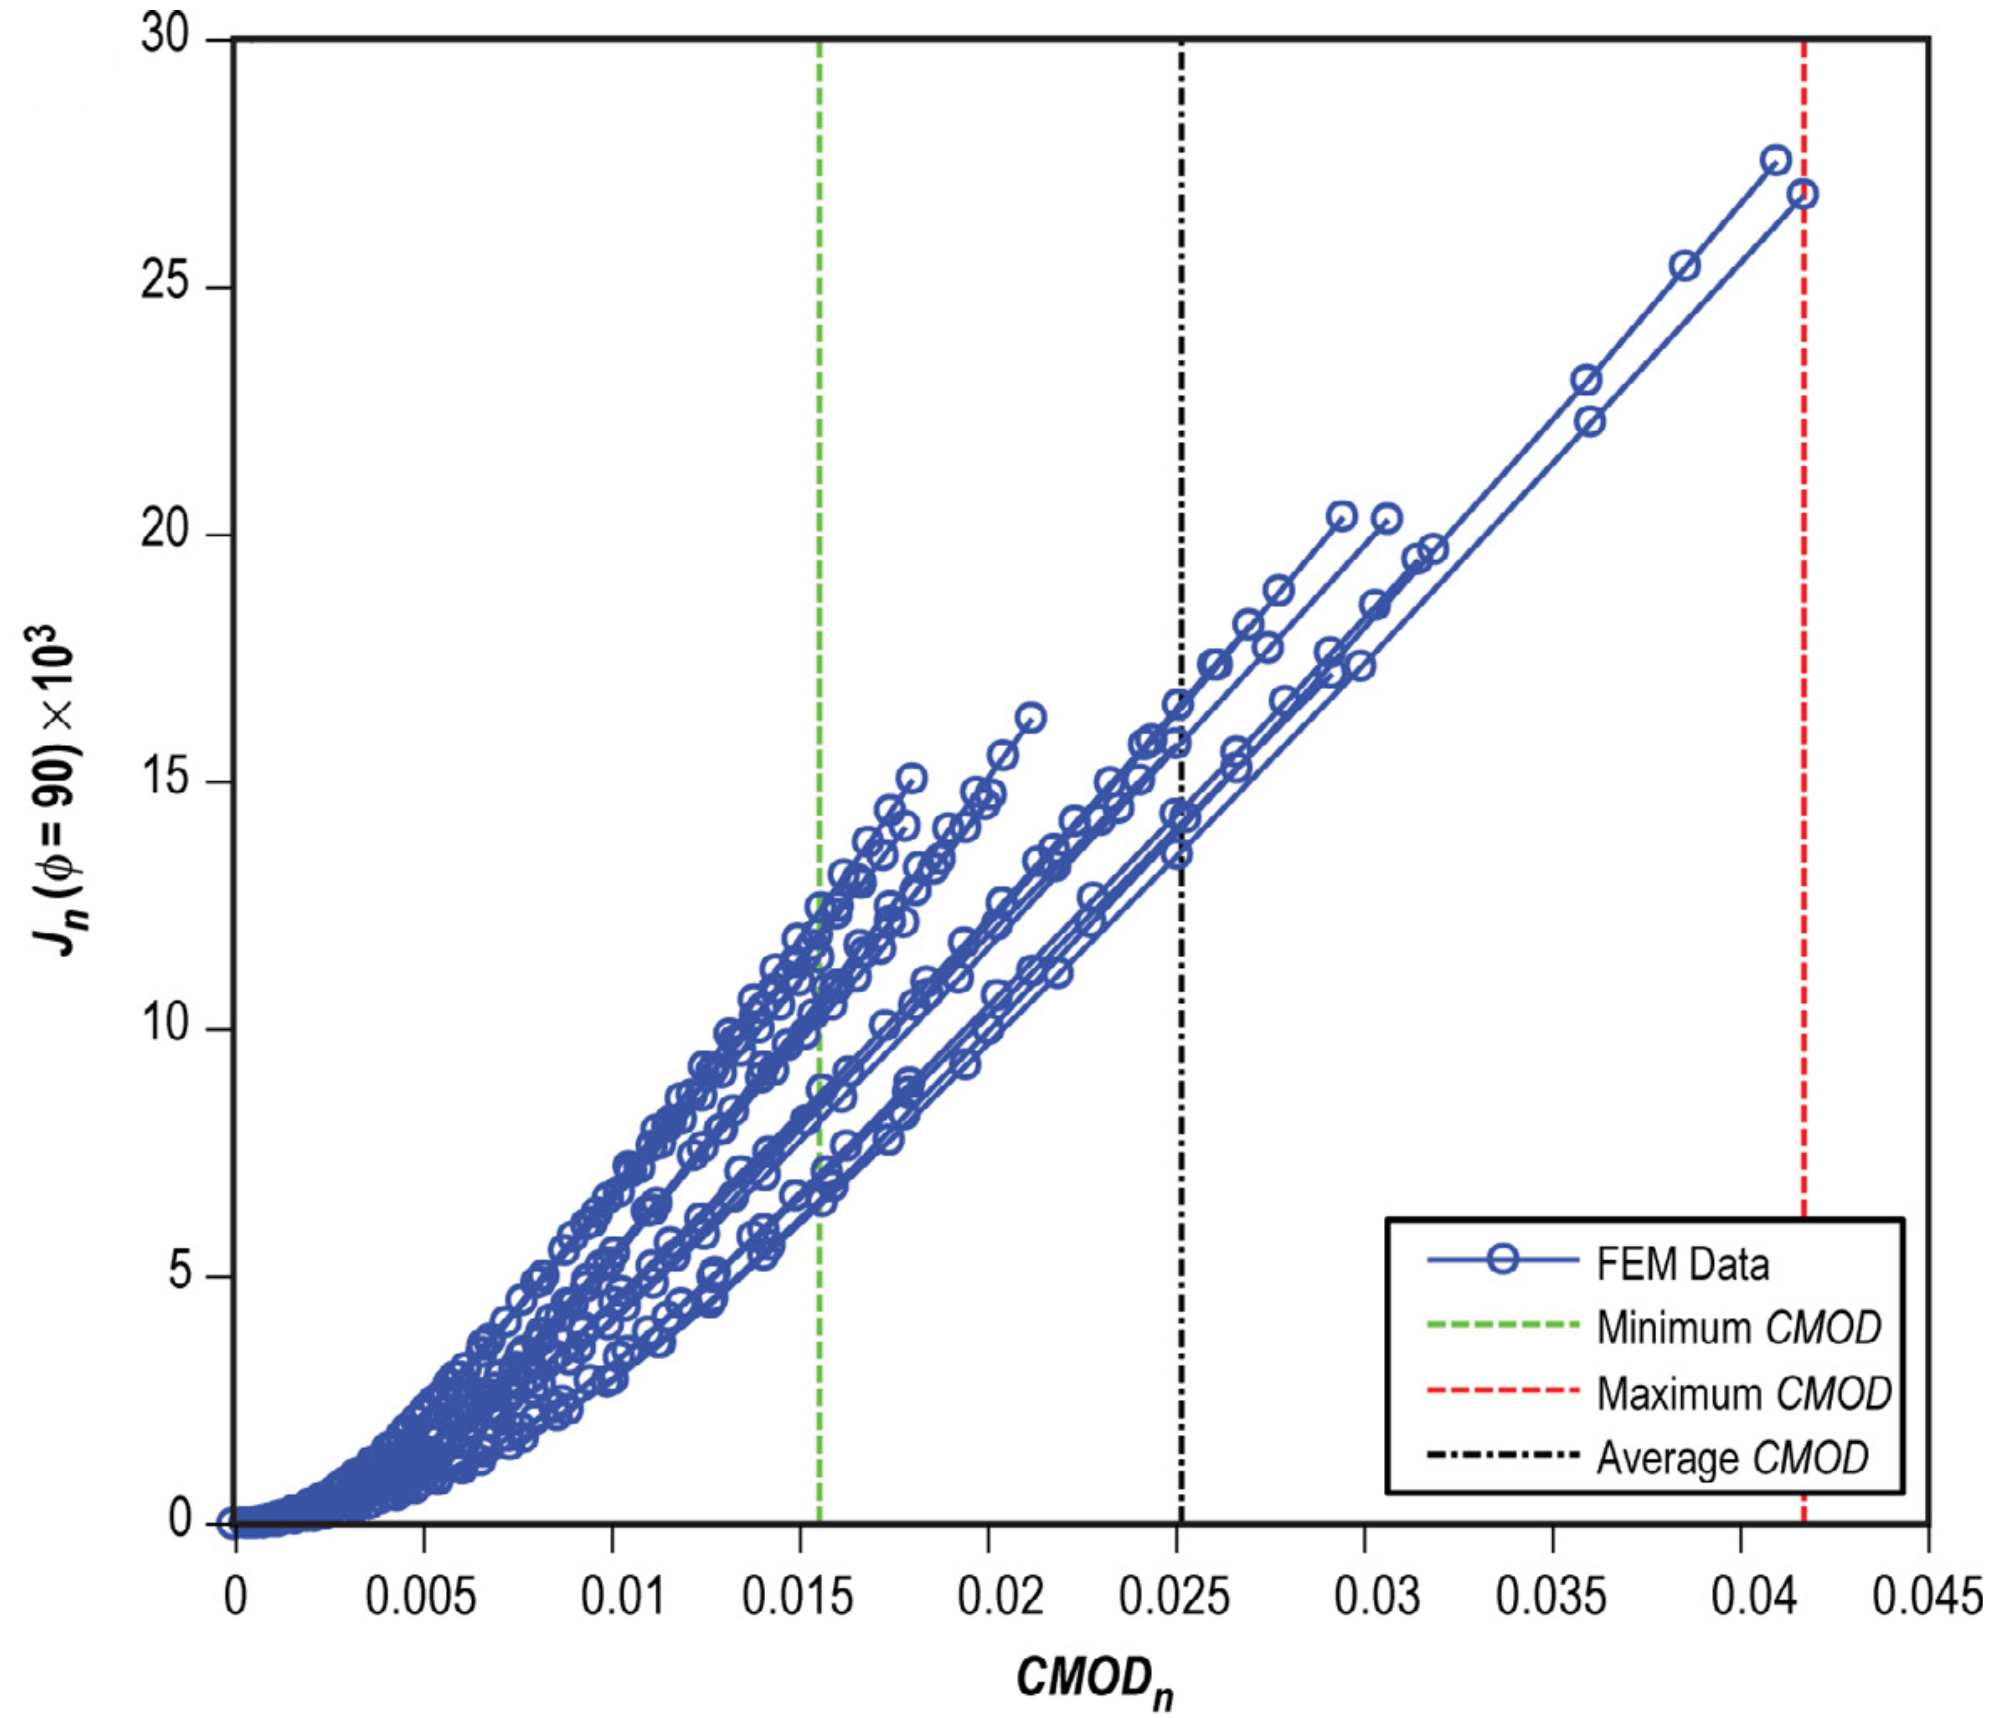
\includegraphics[width=0.7\columnwidth]{J-CMOD-extrapolation}
\caption{\label{fig:J-CMOD-extrapolation} \J-CMOD graph used for extrapolation \cite{allenwells2014}}
\end{figure}

\J{}-CMOD curves like the ones in \Cref{fig:J-CMOD-extrapolation,fig:J-phi-ac_02_at_02_E0100_n03,fig:J-phi-ac_10_at_08_E0500_n06} all show \J values that increase slowly in the linear elastic regime compared to the highly-plastic regime, but have widely varying \J and CMOD ranges. \Cref{fig:J-phi-ac_02_at_02_E0100_n03,fig:J-phi-ac_10_at_08_E0500_n06} show that some cracks in bending show higher \J values at the free surface than deep inside the crack, and others show higher \J values deep inside the crack compared to the free surface.
Since the goal with a bending model is to use enough deformation to make accurate linear extrapolations from the results, the criteria analogous to the \(M\) criteria from \cite{allenwells2014} is defined as
\begin{enumerate} \label{list:criteria}
\item the slope of a linear fit to the last 20\% of the \J-CMOD curve should be at least 20 times larger than the slope of the initial linear region of the \J-CMOD curve, and
\item the slope of the last 20\% of the \J-CMOD curve should be within 10\% of the slope of the previous 20\% of the \J-CMOD curve.
\end{enumerate}
The first criteria ensures that the model has deformed well beyond the linear elastic regime, and the second ensures that a linear extrapolations will be relatively insensitive to additional deformation.
Using ratios of \J and CMOD values in both criteria removes variability due to material properties and crack geometry.
As \J at a given CMOD is a function of angle \(\phi\) from the free surface, the \J values for \(\phi=30{\SIUnitSymbolDegree}\) are used to avoid effects of both the stress-free surface at \SI{0}{\SIUnitSymbolDegree} and constraint effects at \SI{90}{\SIUnitSymbolDegree}.

\begin{figure}[tbp]
\centering
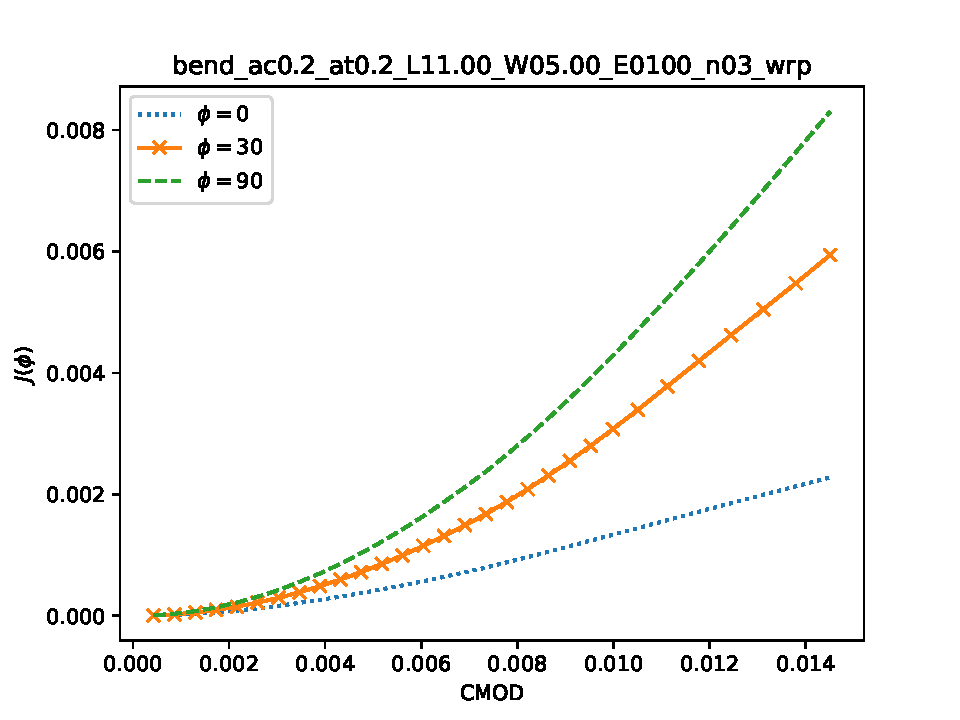
\includegraphics[width=0.8\textwidth]{J_CMOD_bend_ac02_at02_L1100_W0500_E0100_n03_wrp}
\caption{\J-CMOD relationship at \(\phi=\) \SIlist{0;30;90}{\SIUnitSymbolDegree}: \(\frac{a}{c}=0.2\), \(\frac{a}{t}=0.2\), \(E=100\), \(n=3\) \label{fig:J-phi-ac_02_at_02_E0100_n03}}
\end{figure}
\begin{figure}[tbp]
\centering
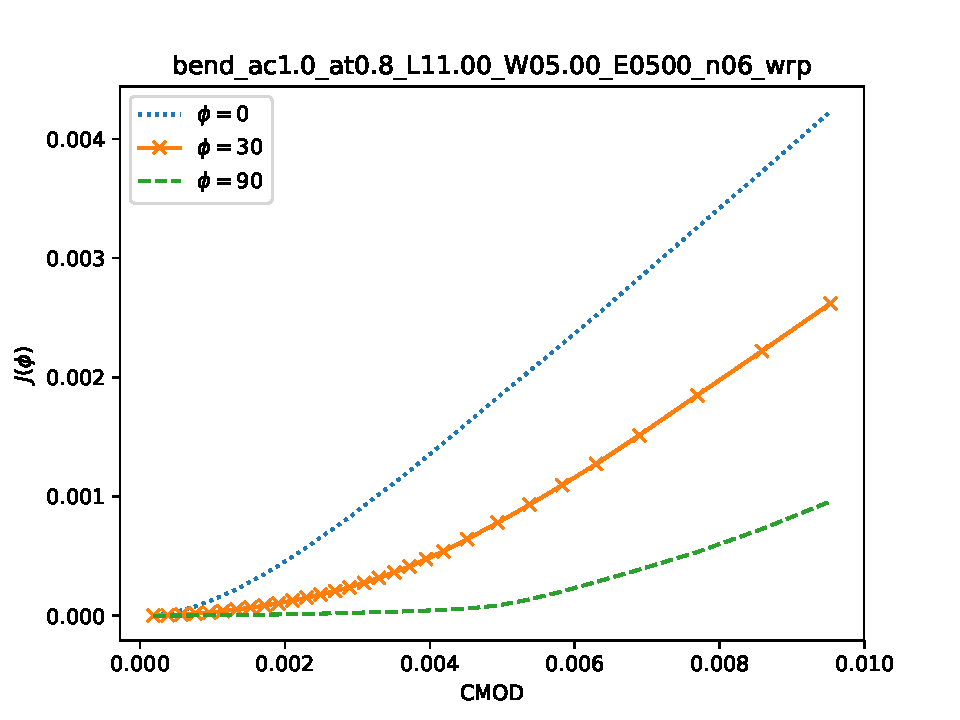
\includegraphics[width=0.8\textwidth]{J_CMOD_bend_ac10_at08_L1100_W0500_E0500_n06_wrp}
\caption{\J-CMOD relationship at \(\phi=\) \SIlist{0;30;90}{\SIUnitSymbolDegree}: \(\frac{a}{c}=1.0\), \(\frac{a}{t}=0.6\), \(E=500\), \(n=6\) \label{fig:J-phi-ac_10_at_08_E0500_n06}}
\end{figure}

An algorithm for for solving a set of models created by \Cref{alg:plate-creator} is shown in \Cref{alg:plate-runner}.
For each combination of \(\frac{a}{c}\), \(\frac{a}{t}\), \(\frac{E}{\sigma_{\text{ys}}}\), and \(n\), it uses \Cref{alg:set_geometry} to calculate the cracked geometry.
It uses \Cref{alg:get_elt_filename,alg:get_generic_model_filename,alg:get_specific_model_filename} to identify relevant input files, and uses \Cref{alg:optimize_bc} to automate the process of modifying boundary conditions and solving the finite element models until the plates have been sufficiently deformed to satisfy the the list of criteria on \cpageref{list:criteria}.
The Python implementation of these algorithms makes use of the \verb|numpy| \cite{numpy}, \verb|scipy| \cite{scipy}, and  \verb|pandas| \cite{mckinney-proc-scipy-2010} libraries.
\verb|scipy| is used for both linear regressions and optimizations, while \verb|pandas| is used for reading structured output files, and for quickly filtering the output.

Looking more closely at the process for finding boundary conditions as shown in \Cref{alg:optimize_bc}, the following details must be considered.
All the materials examined have highly non-linear stress-strain (and load-displacement) behavior, where small changes in applied stresses or loads may cause large changes in strains or displacements.
Similarly, large changes in strain or displacement may only cause small changes in stress or reaction loads.
Displacement boundary conditions were used in \cite{allenwells2014}, which mimics common closed-loop control methods in mechanical properties.
These boundary conditions were constant values applied on the face parallel to the crack front.
However, reaching a sufficient level of plastic deformation around the crack front may require much more displacement than required to reach yield, as shown in \Cref{fig:secant-1}.
\begin{figure}[tbp]
\centering
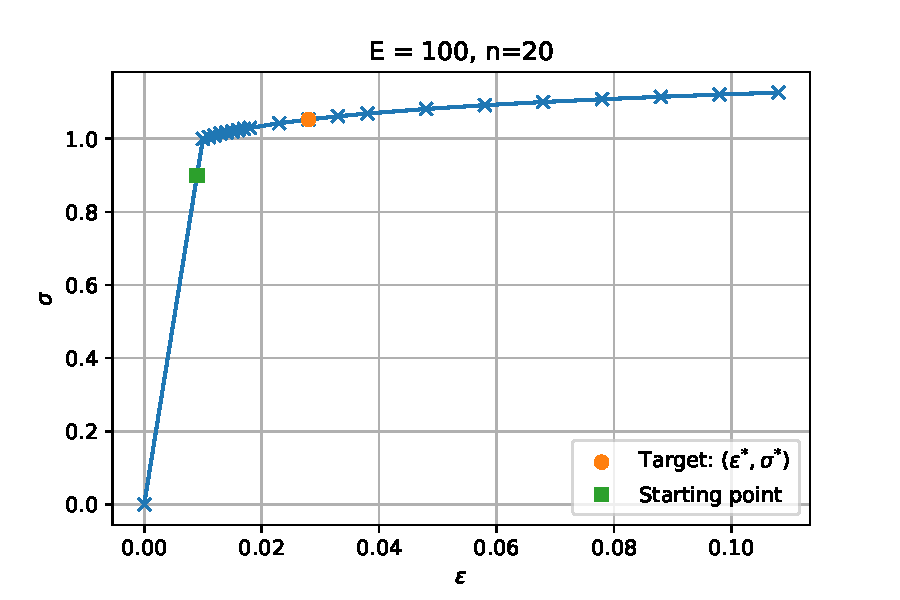
\includegraphics[width=0.8\columnwidth]{secant-1}
\caption{\label{fig:secant-1}Example stress-strain curve using linear plus power law (LPPL) formulation}
\end{figure}
Applying an incremental search to discover how much displacement is required to reach that level of plastic deformation would prove to be slow to converge (where small displacement steps cause even smaller changes in stress state for most of the search space) or inaccurate (where large displacement steps risk running outside the material's defined stress-strain data).
Considering a transformed stress-strain curve as shown in \Cref{fig:secant-2} where the starting point on the stress-strain curve is shown by the green square, the secant method should converge quickly to the target point shown by the orange circle.
\begin{figure}[tbp]
\centering
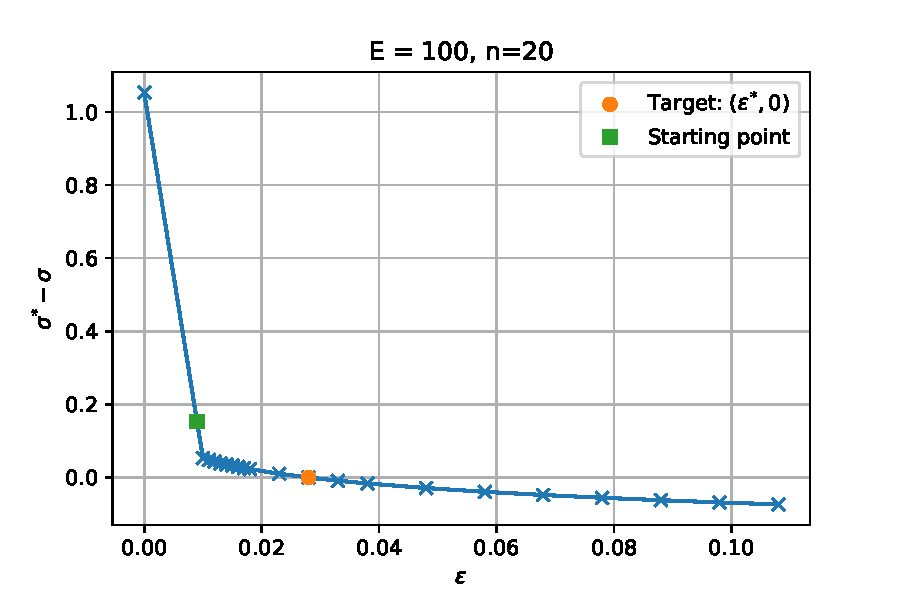
\includegraphics[width=0.8\columnwidth]{secant-2}
\caption{\label{fig:secant-2}LPPL stress-strain curve, transformed to find required strain level}
\end{figure}

The bending models require additional considerations to match experimental conditions, especially for larger plates.
A typical four-point bend test applies external forces with a set of inner cylindrical rollers, and the plate is supported by an outer set of cylindrical rollers, as shown in \Cref{fig:astm-e2899-4point-bend}.
Modeling the internal rollers as constant transverse displacement conditions along a plane parallel to the crack face will grow increasingly inaccurate as that plane rotates relative to the crack face.
Applying transverse tractions on all element faces coincident with the location of the inner roller solves this issue.
And since traction has units of force per unit area, the same traction value can be applied to each element, regardless of the element size.
\begin{figure}[tbp]
\centering
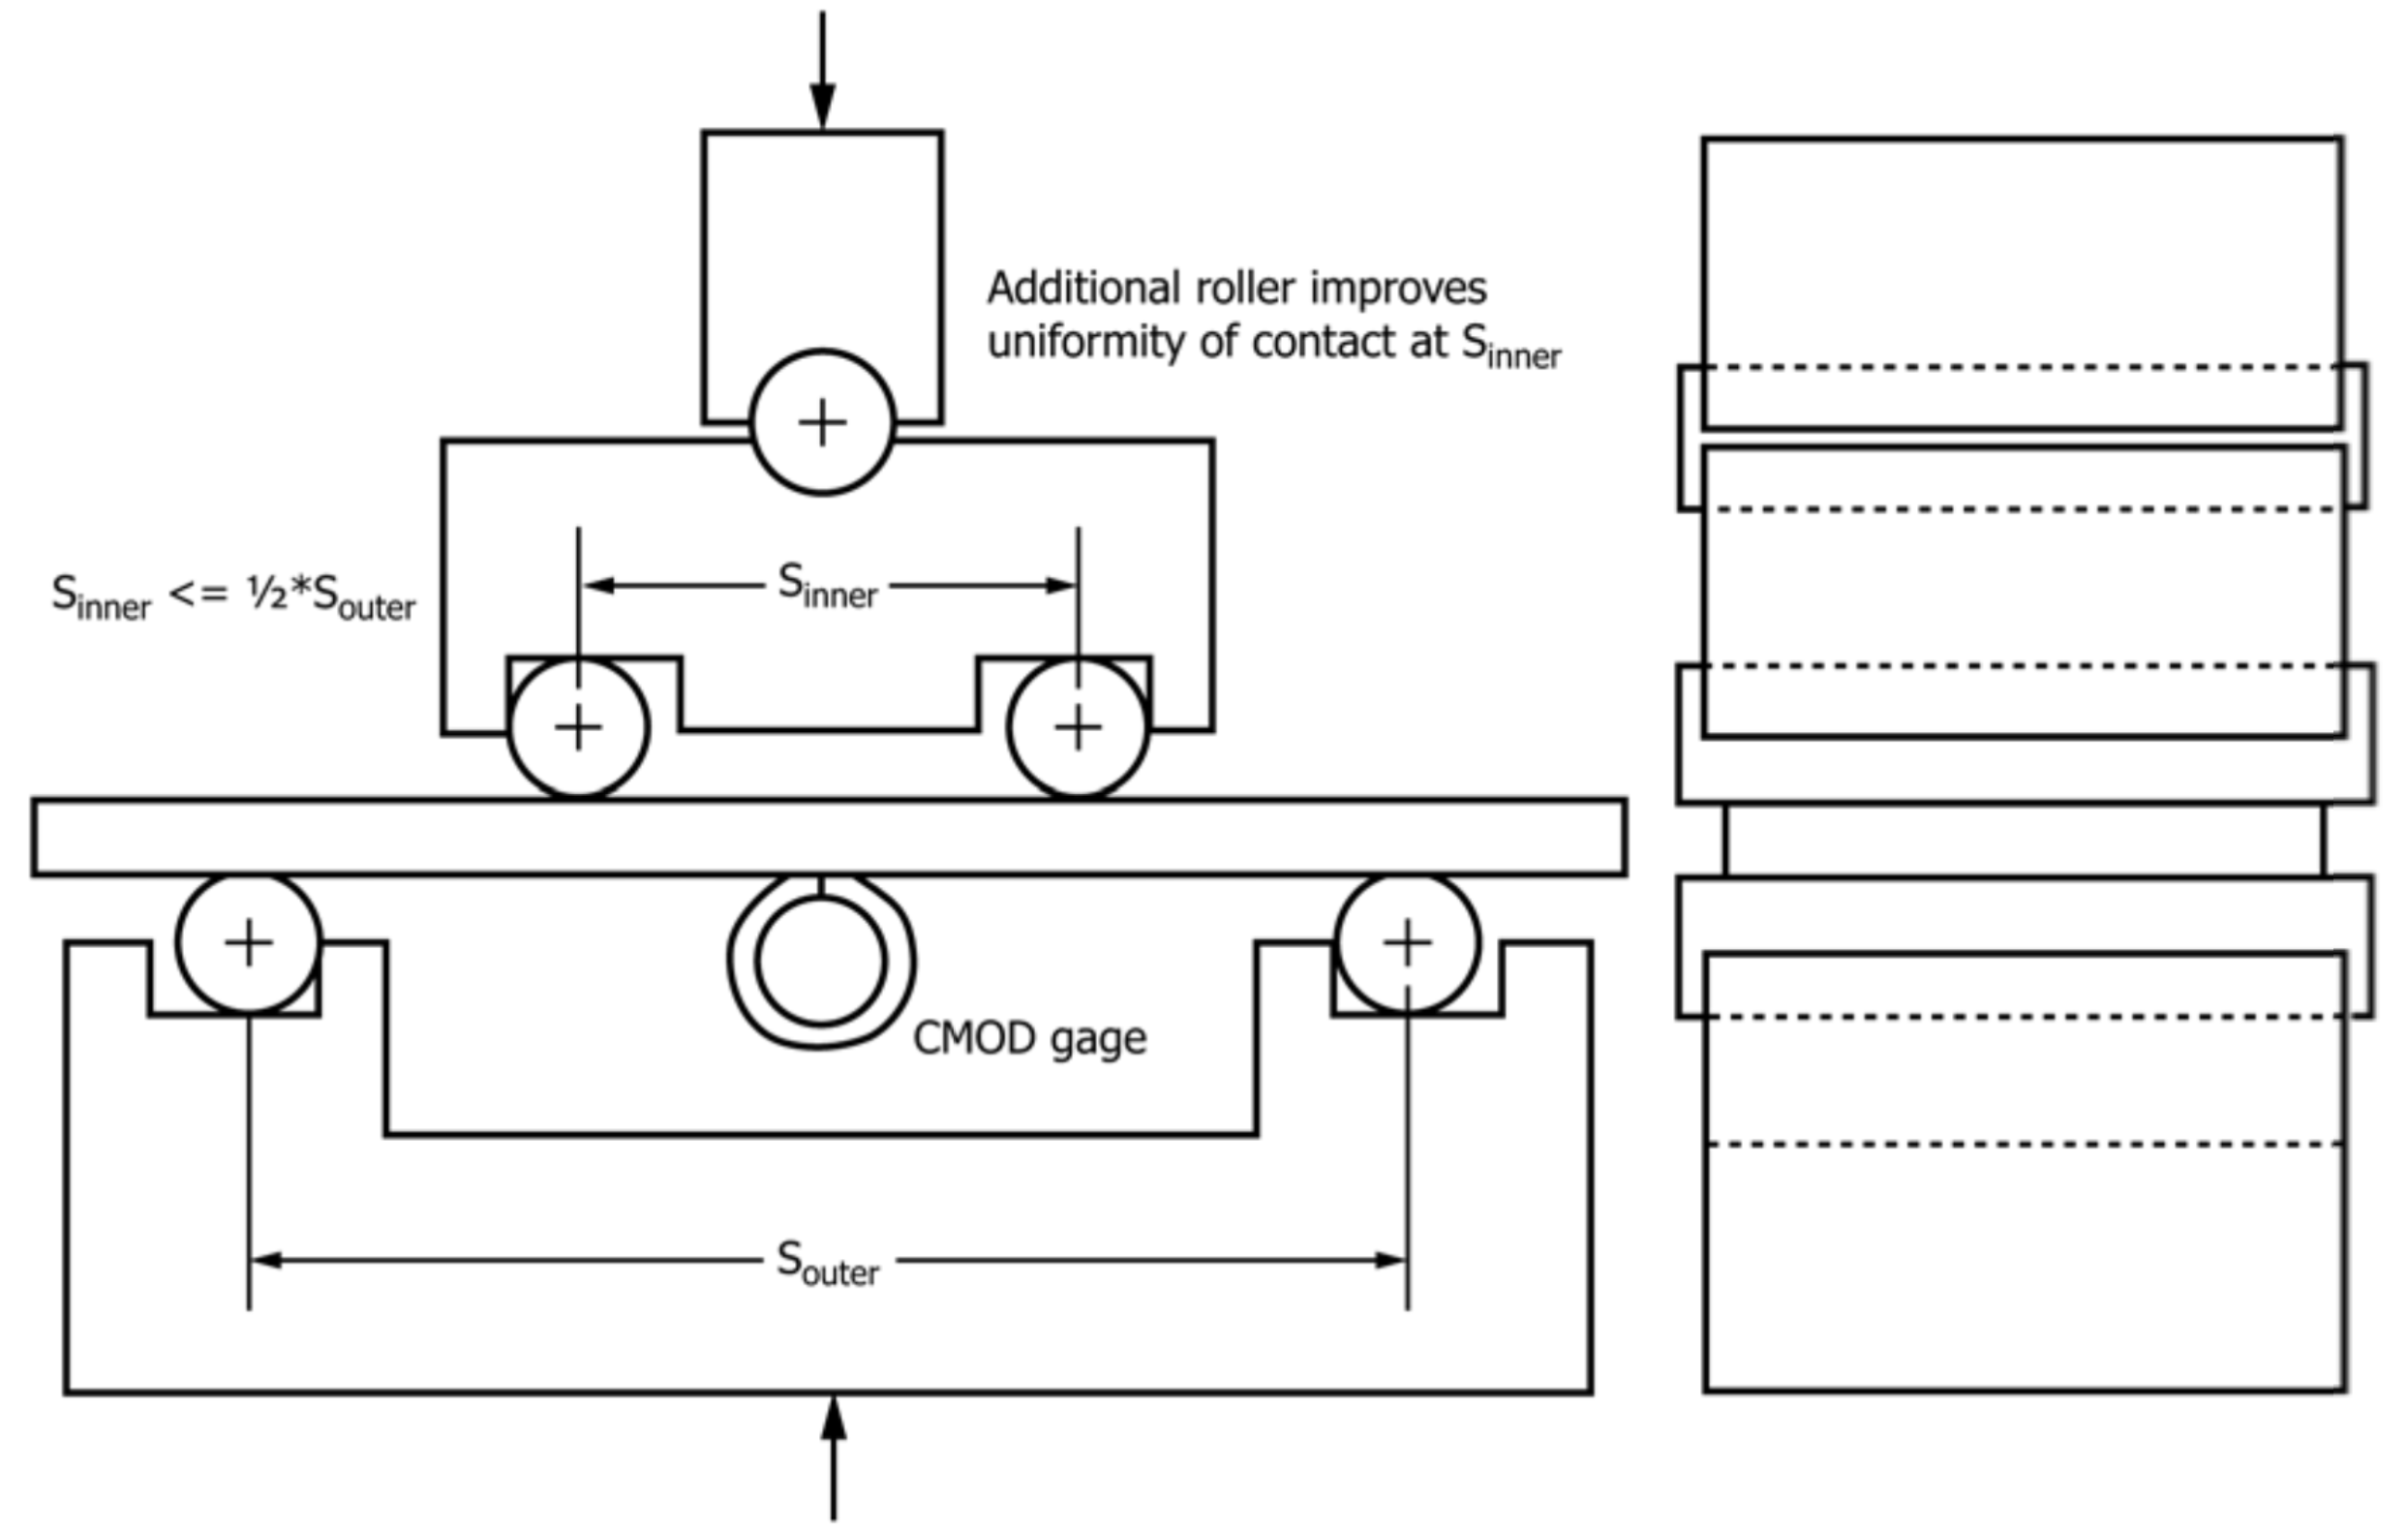
\includegraphics[width=0.8\columnwidth]{astm-e2899-4point-bend}
\caption{\label{fig:astm-e2899-4point-bend} Four-point bend test configuration \cite{astme2899}}
\end{figure}

However, moving from a strain- or displacement-controlled method to a stress- or force-controlled method complicates the root-finding methods used in the tension cases.
As the independent variable is now stress, and the dependent variable is now strain, this transforms the stress-strain curve to the form shown in \Cref{fig:secant-3,fig:secant-4}.
\begin{figure}[tbp]
\centering
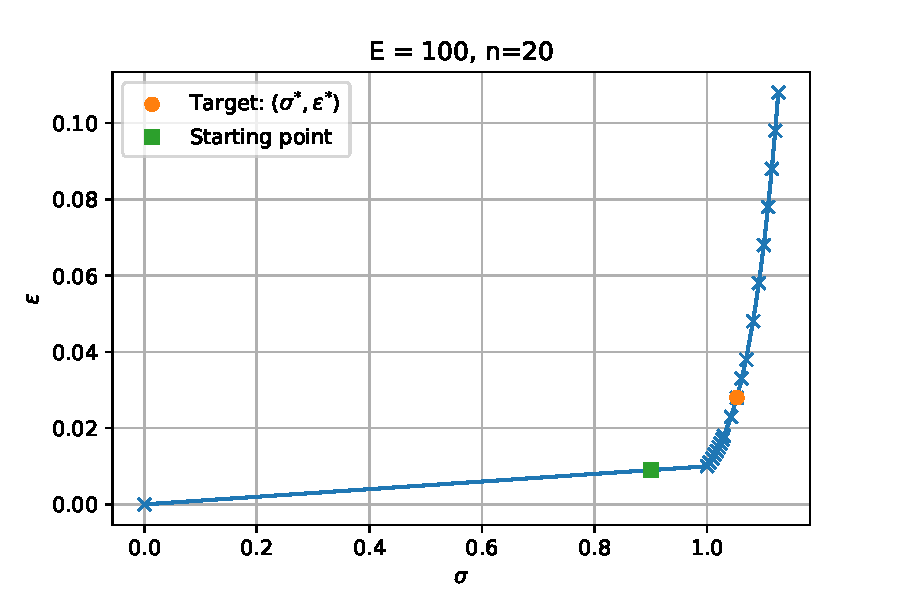
\includegraphics[width=0.8\columnwidth]{secant-3}
\caption{\label{fig:secant-3}Example stress-strain curve using linear plus power law (LPPL) formulation, transformed to stress-controlled}
\end{figure}
\begin{figure}[tbp]
\centering
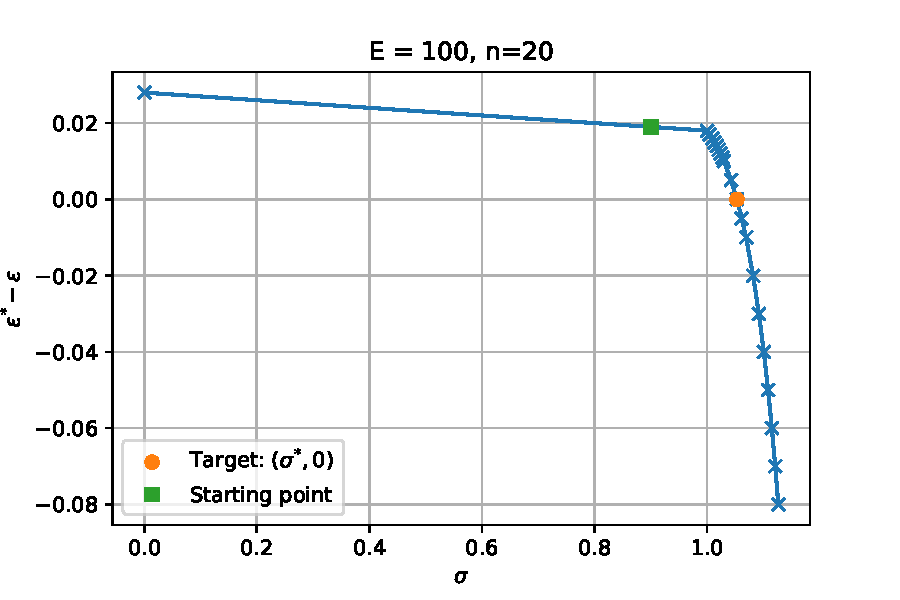
\includegraphics[width=0.8\columnwidth]{secant-4}
\caption{\label{fig:secant-4}Example stress-strain curve using linear plus power law (LPPL) formulation, transformed to find required stress level}
\end{figure}
The curve is now much less suitable for solution using the secant method: the neighborhood of starting point has a very shallow slope that will cause the next stress value to be much higher, either causing slow convergence in the case of an LPPL function with a semi-infinite domain, or simply exceeding the range of the stress-strain curve in the case of a finite set of stress-strain points.
However, using a simple incremental search method with step sizes equal to 10\% of the initial stress only takes a few steps to reach the neighborhood of the target stress value.
Other root-finding methods could be used to find the required stress value, such as bisection, false position, or Brent's method.
However, each of these methods requires the determination of a finite interval \([\sigma_a, \sigma_b]\) that surround the required stress value.
Though it is possible to set that interval to the domain of a finite set of stress-strain data points, but this is impossible for an LPPL function with a semi-infinite domain.
Additionally, the open-ended nature of the slope ratio criteria on \cpageref{list:criteria} means that all stress values exceeding a minimum target value will meet that criteria.
Finally, having a finite number of load steps in the finite element model and the need to accurately model the transition to elastic-plastic behavior means that lower stress values meeting the criteria on \cpageref{list:criteria} are preferred.
All three of these factors lead to a conclusion that any root-finding method that requires no bracketing and whose proposed root values monotonically increase will find appropriate stress values that will allow accurate extrapolation without sacrificing detail in the transition to elastic-plastic behavior.
\begin{algorithm}[tbp]
  \caption{Plate Runner}
  \label{alg:plate-runner}
  \begin{algorithmic}
    \Procedure{Plate Runner}{} \Comment{Solve a series of WARP3D input files}
    \State Read lists of $\frac{a}{t}$, $\frac{a}{c}$, $\frac{E}{\sigma_{\text{ys}}}$, $n$ values from configuration
    \State \Comment{typically: $0.2 \leq \frac{a}{t} \leq 0.8$, $0.2 \leq \frac{a}{c} \leq 1.0$, $100 \leq \frac{E}{\sigma_\text{ys}} \leq 1000$, $3 \leq n \leq 20$}
    \State Read $t$, $\sigma_\text{ys}$, global .elt file from configuration
    \State \Comment{typically: $t=1$, $\sigma_\text{ys}=1$, and global .elt file = 'bend.elt'}
    \ForAll{($\frac{a}{t}$ values, $\frac{a}{c}$ values)}
      \State $(a, c, L, W, S_{\text{in}}, S_{\text{out}}) \gets \Call{Set Geometry}{\text{global .elt file}, \frac{a}{c}, \frac{a}{t}, t}$
      \ForAll{($\frac{E}{\sigma_\text{ys}}$ values, $n$ values)}
        \State $E \gets (\frac{E}{\sigma_\text{ys}})(\sigma_\text{ys})$
        \State {model .elt file} $\gets$ \Call{Get Elt Filename}{{global .elt file}, $a$, $c$, $L$, $W$, $t$} 
        \State \Comment{'bend\_ac$(\frac{a}{c})$\_at$(\frac{a}{t})$\_L$(L)$\_W$(W)$.elt'}
        \State {generic .inp file} $\gets$ \Call{Get Generic Model Filename}{{model .elt file}}
        \State \Comment{'bend\_ac$(\frac{a}{c})$\_at$(\frac{a}{t})$\_L$(L)$\_W$(W)$\_wrp.inp'}
        \State {specific .inp file} $\gets$ \Call{Get Specific Model Filename}{{generic .inp file}, $E$, $\sigma_\text{ys}$, $n$}
        \State \Comment{'bend\_ac$(\frac{a}{c})$\_at$(\frac{a}{t})$\_L$(L)$\_W$(W)$\_E$(E)$\_n$(n)$\_wrp.inp'}
        \If{\Call{Get Model Type}{specific .inp file} = 'bending'}
          \State ($z_{\text{in}}$, $z_{\text{out}}$) = \Call{Find Pin Locations}{specific .inp file}
%\todo[inline]{This needs cleaned up -- if Sin and Sout are not None, zin and zout are just Sin/2 and Sout/2, respectively.}
        \EndIf
        \State \Call{Optimize BC}{specific .inp file, $a$, $c$, $L$, $W$, $t$, $z_{\text{in}}$, $z_{\text{out}}$, $E$, $n$}
        \State \Call{Postprocess}{specific .inp file}
      \EndFor
    \EndFor
    \EndProcedure
  \end{algorithmic}
\end{algorithm}

\begin{algorithm}[tbp]
  \caption{Get Generic Model Filename}
  \label{alg:get_generic_model_filename}
  \begin{algorithmic}
    \Procedure{Get Generic Model Filename}{model .elt file}
    \State prefix $\gets$ model .elt file basename \Comment{'bend\_ac$(\frac{a}{c})$\_at$(\frac{a}{t})$\_L$(L)$\_W$(W)$'}
    \State \textbf{return} prefix + '\_wrp.inp' \Comment{'bend\_ac$(\frac{a}{c})$\_at$(\frac{a}{t})$\_L$(L)$\_W$(W)$\_wrp.inp'}
\EndProcedure
  \end{algorithmic}
\end{algorithm}

\begin{algorithm}[tbp]
  \caption{Optimize BC}
  \label{alg:optimize_bc}
  \begin{algorithmic}
    \Procedure{Optimize BC}{.inp file, $a$, $c$, $L$, $W$, $t$, $z_{\text{in}}$, $z_{\text{out}}$, $E$, $\sigma_{\text{ys}}$, $n$}
    \State \Comment{Change Boundary Conditions for Model until Sufficient Deformation Applied}
    \State model type $\gets$ \Call{Get Model Type}{.inp file} %\todo[inline]{This needs cleaned up. Set model type based off values of $z_{\text{in}}$, $z_{\text{out}}$.}
    \State initial BC $\gets$ \Call{Get Initial BC}{.inp file, $a$, $c$, $L$, $W$, $t$, $z_{\text{in}}$, $z_{\text{out}}$, $E$, $\sigma_{\text{ys}}$, $n$, model type}
    \If{model type = 'tension'}
      \State optimal BC $\gets$ \Call{Secant Method}{\Call{Run Model}{initial BC}}
      \State \Comment{with fixed values for .inp file, $a$, $c$, $L$, $W$, $t$, $z_{\text{in}}$, $z_{\text{out}}$, $E$, $n$, model type}
    \Else
      \State BC $\gets$ initial BC
      \While{$\Call{Run Model}{\text{initial BC}}>0$}
        \State \Comment{with fixed values for .inp file, $a$, $c$, $L$, $W$, $t$, $z_{\text{in}}$, $z_{\text{out}}$, $E$, $n$, model type}
        \State BC $\gets$ BC + 0.1 (initial BC)
      \EndWhile
      \State optimal BC $\gets$ BC
    \EndIf
    \State \textbf{return} optimal BC
    \EndProcedure
  \end{algorithmic}
\end{algorithm}

\Cref{alg:optimize_bc} uses \Cref{alg:get_model_type} to determine if the model being solved is under tension or bending loads, and then uses \Cref{alg:get_initial_bc} to calculate the initial boundary condition required to cause a net section stress of 0.9\Sys.
It then passes that initial boundary condition to the objective function given in \Cref{alg:run_model}, modifying the boundary condition until the objective function returns a value of 0.
The objective function itself first verifies that the applied boundary condition is positive, and if not, immediately returns a value high enough to push any optimization method away from negative boundary condition values.
For a positive boundary condition value, it calls \Cref{alg:modify_bc} to modify the WARP3D input file, finds any existing binary packet files defined by \Cref{alg:get_bpf_filename} and removes them, and then runs WARP3D using the modified input file.

Once WARP3D exits, it examines the output file for evidence of a terminated analysis.
If the analysis was terminated abnormally, typically due to exceeding strain limits, it returns a value high enough to push any optimization toward lower boundary condition values.
If the analysis ran successfully, it reads \J and \(\phi\) values for each load step from the input and output files with \Cref{alg:find_j}, and extracts nodal displacements from the binary packet file with \Cref{alg:extract_results}.

The displacement for the node at \((x, y, z) = (0, 0, 0)\) is used to calculate the CMOD using \Cref{alg:get_mesh_filename,alg:get_nodal_results,alg:get_node_coordinates,alg:get_cmod}, and an interpolated value for \J at \(\phi=30{\SIUnitSymbolDegree}\) is calculated with \Cref{alg:interpolate_j}.
Finally, the \J, CMOD, and boundary values are passed to the primary objective function given in \Cref{alg:j_cmod_objective}.
That objective function first normalizes the \J and CMOD values to lie within an interval of \([0, 1]\).
As the distribution of points along the \J-CMOD curve are typically biased toward the early part of the curve as applied boundary conditions grow higher, there's a chance that the final 40\% of the \J-CMOD curve may only contain a small number of points, as can be seen in \Cref{fig:J-phi-ac_10_at_08_E0500_n06}.
To correct for this, a set of 50 evenly spaced interpolation points are defined along the \J-CMOD curve.
This gives 20 points for calculating the slope of the \J-CMOD curve in the elastic-plastic regime, providing more stable objective function values.

The interpolated values are used to calculate slopes of the \J-CMOD curve for normalized CMOD values on the intervals \([0.6, 0.8)\) and \([0.8, 1.0]\).
The relative amount of change between those two slopes and the ratio of the last interval's slope to the slope of the linear region is used to calculate an objective value.
If the amount of change is under 10\%, and the slope ratio exceeds 20, an objective value of 0 is returned.
Otherwise, an objective value of the relative change divided by the ratio is returned.
This has the effect of encouraging steeper slopes in the elastic-plastic regime, and also graphs providing more accurate linear extrapolation for CMOD values beyond those modeled.

\begin{algorithm}[tbp]
  \caption{Get Model Type}
  \label{alg:get_model_type}
  \begin{algorithmic}
    \Procedure{Get Model Type}{.inp file}
    \State \Comment{first, check for non-zero displacement constraints in the $z$ direction for tension models}
    \State start index $\gets$ Index of first line of input file matching 'constraints'
    \State end index $\gets$ Index of next line of input file matching 'c* echo off'
    \ForAll{input file lines between start index and end index}
      \If{line contains $w$ constraint} \Comment{$z$ direction constraint}
        \If{$w$ constraint value $\neq 0$} \Comment{plate deformed in $z$ direction}
          \State \textbf{return} 'tension'
        \EndIf
      \EndIf
    \EndFor
    \State \Comment{then, check for non-zero tractions applied in the $y$ direction for bending models}
    \State start index $\gets$ Index of first line of input file matching 'loading set1'
    \State end index $\gets$ Index of next line of input file matching 'c'
    \ForAll{input file lines between start index and end index}
      \If{line contains 'ty'} \Comment{$y$ direction traction}
        \If{$y$ direction traction value $\neq 0$} \Comment{plate deformed in $y$ direction}
          \State \textbf{return} 'bending'
        \EndIf
      \EndIf
    \EndFor
    \State \textbf{raise exception} 'Could not detect model type'
    \State \Comment{If we get this far, the .inp file represents something outside our model space}
    \EndProcedure
  \end{algorithmic}
\end{algorithm}

\begin{algorithm}[tbp]
  \caption{Get Initial BC}
  \label{alg:get_initial_bc}
  \begin{algorithmic}
    \Procedure{Get Initial BC}{.inp file, $a$, $c$, $L$, $W$, $t$, $z_{\text{in}}$, $z_{\text{out}}$, $E$, $\sigma_{\text{ys}}$, $n$, model type}
    \State ratio $\gets$ 0.9 \Comment{net section stress desired in uncracked body relative to $\sigma_{\text{ys}}$}
    \If{model type = 'tension'}
    %\todo[inline]{This needs cleaned up. Set model type based off values of $z_{\text{in}}$, $z_{\text{out}}$.}
      \State initial BC $\gets$ $(\text{ratio}) \sigma_{\text{ys}} \frac{L}{E}$ \Comment{$w = \frac{PL}{AE} = (\frac{P}{A})(\frac{L}{E}) = \sigma \frac{L}{E}$}
    \Else
      \State $\bar{y}$ $\gets$ $y$ centroid of plate cross section
      \State $I$ $\gets$ second moment of area of plate cross section with respect to $x$ axis
      \State initial BC $\gets$ $-(\text{ratio}) \sigma_{\text{ys}} \frac{I}{W t \bar{y} (z_{\text{outer}}-z_{\text{inner}})}$
      \State \Comment{$\sigma = -\frac{M y}{I} = \frac{P(z_{\text{outer}}-z_{\text{inner}})y}{I} = -\frac{(\text{traction }W t) (z_{\text{outer}}-z_{\text{inner}})y}{I}$}
      \State \Comment{$\text{traction} = - \sigma \frac{I}{W t y (z_{\text{outer}}-z_{\text{inner}})}$}
    \EndIf
    \State \textbf{return} initial BC
    \EndProcedure
  \end{algorithmic}
\end{algorithm}

\begin{algorithm}[tbp]
  \caption{Run Model}
  \label{alg:run_model}
  \begin{algorithmic}
    \Procedure{Run Model}{BC, .inp file, $a$, $c$, $L$, $W$, $t$, $z_{\text{in}}$, $z_{\text{out}}$, $E$, $n$, model type}
    \If{$\text{BC} \leq 0$}
      \State objective $\gets$ $-\text{BC}+0.1$
      \State \Comment{Non-positive BCs not allowed. Push BC back towards positive values.}
    \Else
      \State{\Call{Modify BC}{BC, input file, model type}}
      \State input basename $\gets$ basename of .inp file \Comment{'bend\_ac$(\frac{a}{c})$\_at$(\frac{a}{t})$\_L$(L)$\_W$(W)$\_wrp'}
      \State output filename $\gets$ input basename + '.out' \Comment{'bend\_ac$(\frac{a}{c})$\_at$(\frac{a}{t})$\_L$(L)$\_W$(W)$\_wrp.out'}
      \State BPF filename $\gets$ \Call{Get BPF Filename}{input file}
      \If{BPF file already exists}
        \State Remove BPF file
      \EndIf
      \State Run WARP3D, reading input file, writing output file
      \State output lines $\gets$ read output file
      \If{output lines contains 'analysis terminated'}
        \State objective $\gets$ $\text{BC}-0.01$ \Comment{Probably exceeded strain limits. Push BC lower.}
      \Else
        \State input lines $\gets$ read input file
        \State $\phi$, \J $\gets$ \Call{Find \J}{input lines, output lines}
        \State \Comment{table of \J values (one value per combination of $\phi$ and load step)}
        \State output filenames $\gets$ \Call{Extract Results}{BPF filename}
        \State \Comment{a dictionary containing names of reaction and displacement result files}
        \State node file $\gets$ \Call{Get Mesh Filename}{input file}
%        \State reaction table $\gets$ \Call{Get Nodal Results}{reaction result filename}
        \State node table $\gets$ \Call{Get Node Coordinates}{node file}
    	\State CMOD $\gets$ \Call{Get CMOD}{node table, displacement result filename, 0, 0, 0}
        \State $\J(\phi=30{\SIUnitSymbolDegree})$ $\gets$ \Call{Interpolate \J}{$\phi$, \J, $\frac{\pi}{6}$}
        \State objective $\gets$ $(\frac{1}{\text{BC}})$ $(\Call{\J-CMOD Objective}{\J(\phi=30{\SIUnitSymbolDegree}), \text{CMOD}})$
        \State \Comment{divide by BC to counter inflections in \J-CMOD curves that increase objective locally}
      \EndIf
    \EndIf
    \State \textbf{return} objective
    \EndProcedure
  \end{algorithmic}
\end{algorithm}

\begin{algorithm}[tbp]
  \caption{Modify BC}
  \label{alg:modify_bc}
  \begin{algorithmic}
    \Procedure{Modify BC}{BC, input file, model type}
    \State input lines $\gets$ read input file
    \If{model type = 'tension'}
      \State find constraint lines in input lines
      \ForAll{line in constraint lines}
        \If{\(w\) value is constrained \AND \(w\) value $\neq$ 0}
          \State search and replace \(w\) value with BC
        \EndIf
      \EndFor
    \Else \Comment{model type = 'bending'}
      \State find loading set lines in input lines
      \ForAll{line in loading set lines}
        \If{traction \(y\) value is constrained \AND traction \(y\) value $\neq$ 0}
          \State search and replace \(w\) value with BC
        \EndIf
      \EndFor
    \EndIf
    \State input file $\gets$ write input lines
    \EndProcedure
  \end{algorithmic}
\end{algorithm}

\begin{algorithm}[tbp]
  \caption{Get BPF Filename}
  \label{alg:get_bpf_filename}
  \begin{algorithmic}
    \Procedure{Get BPF Filename}{.inp file}
      \State prefix $\gets$ .inp file basename \Comment{'bend\_ac$(\frac{a}{c})$\_at$(\frac{a}{t})$\_L$(L)$\_W$(W)$\_E$(E)$\_n$(n)$\_wrp'}
      \State prefix $\gets$ prefix without last 4 characters \Comment{'bend\_ac$(\frac{a}{c})$\_at$(\frac{a}{t})$\_L$(L)$\_W$(W)$\_E$(E)$\_n$(n)$'}
      \State suffix $\gets$ '.bpf'
      \State \textbf{return} prefix + suffix \Comment{'bend\_ac$(\frac{a}{c})$\_at$(\frac{a}{t})$\_L$(L)$\_W$(W)$\_E$(E)$\_n$(n)$.bpf'}
    \EndProcedure
  \end{algorithmic}
\end{algorithm}

\begin{algorithm}[tbp]
  \caption{Find \J}
  \label{alg:find_j}
  \begin{algorithmic}
    \Procedure{Find \J}{input lines, output lines}
    \State start index $\gets$ Index of first input line matching 'c  Analysis Load Step Data'
    \State steps $\gets$ last field of input line ((start index)+1)
    \State start index $\gets$ Index of first input line matching 'c  Crack Node Data'
    \State crack node count $\gets$ last field of input line (start index)+14)
    \State \Comment{crack node count includes midside nodes, but \J only calculated for corner nodes}
    \State $\phi$ $\gets$ vector of zeroes \Comment{length equal to ((crack node count)+1)/2}
    \State \J $\gets$ array of zeroes \Comment{rows equal to steps, columns equal to length($\phi$)}
    \State \J contour label list $\gets$ empty list
    \State $j$ $\gets$ 0
    \For{i $\gets$ (start index)+16, (start index)+16+(crack node count), 2}
      \State $\phi_j$, label $\gets$ fields 3 and 4 of input line $i$
      \State $\phi(j)$ $\gets$ $\phi_j$ \Comment{places current $\phi$ value into $\phi$ vector}
      \State Append label to \J contour label list
      \State $j$ $\gets$ $j+1$
    \EndFor
    \State start index $\gets$ 0
    \For{step $\gets$ 0, steps}
      \State start index $\gets$ Index of next input line containing 'loading: history1     step:'
      \ForAll{label in \J contour label list}
        \State{column $\gets$ Index of label in \J contour label list}
        \State{row $\gets$ step}
        \State start index $\gets$ Index of next output line containing 'average      minimum      maximum'
        \State \J(row, column) $\gets$ field 3 of output line (start index)+1
      \EndFor
    \EndFor
    \Return $\phi$, \J
    \EndProcedure
  \end{algorithmic}
\end{algorithm}

\begin{algorithm}[tbp]
  \caption{Extract Results}
  \label{alg:extract_results}
  \begin{algorithmic}
    \Procedure{Extract Results}{BPF filename}
    \State BPF basename $\gets$ basename of BPF filename
    \Comment{'bend\_ac$(\frac{a}{c})$\_at$(\frac{a}{t})$\_L$(L)$\_W$(W)$\_E$(E)$\_n$(n)$'}
    \State results map $\gets$ [('displacements', 1), ('reactions', 4)]
    \State filename dictionary $\gets$ empty dictionary
    \ForAll{(kind, code) in results map}
      \State output filename $\gets$ BPF basename + '-' + kind + '.out'
      \State \Comment{e.g., 'bend\_ac$(\frac{a}{c})$\_at$(\frac{a}{t})$\_L$(L)$\_W$(W)$\_E$(E)$\_n$(n)$-displacements.out'}
      %\todo[inline]{Need to remove any existing output file before running packet\_reader.}
      \State \Comment{packet\_reader normally requires keyboard input}
      \State input bytes $\gets$ byte array of input lines
      \State \Comment{input lines: BPF filename, result code, 'n', and output filename}
      \State Run packet\_reader, providing keyboard input from input bytes
      %\todo[inline]{subprocess.run() might be easier than making byte array and using Popen}
      \State filename dictionary[kind] $\gets$ output filename
    \EndFor
    \State \Return filename dictionary
    \EndProcedure
  \end{algorithmic}
\end{algorithm}

\begin{algorithm}[tbp]
  \caption{Get Mesh Filename}
  \label{alg:get_mesh_filename}
  \begin{algorithmic}
    \Procedure{Get Mesh Filename}{.inp file}
    \State inp basename $\gets$ basename of .inp filename
    \Comment{'bend\_ac$(\frac{a}{c})$\_at$(\frac{a}{t})$\_L$(L)$\_W$(W)$\_E$(E)$\_n$(n)$\_wrp'}
    \State prefix $\gets$ basename without last 4 characters \Comment{'bend\_ac$(\frac{a}{c})$\_at$(\frac{a}{t})$\_L$(L)$\_W$(W)$\_E$(E)$\_n$(n)$'}
    \State base $\gets$ prefix split by \_ characters, all but last two fields
    \Comment{'bend\_ac$(\frac{a}{c})$\_at$(\frac{a}{t})$\_L$(L)$\_W$(W)$'}
    \State suffix $\gets$ '\_msh.out'
    \State \Return base + suffix \Comment{'bend\_ac$(\frac{a}{c})$\_at$(\frac{a}{t})$\_L$(L)$\_W$(W)$\_msh.out'}
    \EndProcedure
  \end{algorithmic}
\end{algorithm}

\begin{algorithm}[tbp]
  \caption{Get Nodal Results}
  \label{alg:get_nodal_results}
  \begin{algorithmic}
  \Procedure{Get Nodal Results}{filename}
  \State table $\gets$ Pandas read\_table(filename, space separated, treat 'TOT' lines as 'N/A')
  \State table $\gets$ Drop N/A values from table
  \State final table $\gets$ empty table
  \ForAll{step in unique values of 'step' column from table}
    \State table step $\gets$ all table rows where 'step' column = step
    \State Renumber 'node' column of table step starting at 1
    \State \Comment{Some models overflow the space allotted for node numbering}
    \State Append table step to final table
  \EndFor
  \State \Return final table
  \EndProcedure
  \end{algorithmic}
\end{algorithm}

\begin{algorithm}[tbp]
  \caption{Get Node Coordinates}
  \label{alg:get_node_coordinates}
  \begin{algorithmic}
  \Procedure{Get Node Coordinates}{mesh filename}
  \State mesh stats $\gets$ Pandas read\_table(mesh filename, space separated, skip 4 rows, read 1 row)
  \State $n$ $\gets$ first field of mesh stats
  \State coordinates $\gets$ Pandas read\_table(mesh filename, space separated, skip 10 rows, read $n$ rows)
  \State \Return coordinates
  \EndProcedure
  \end{algorithmic}
\end{algorithm}

\begin{algorithm}[tbp]
  \caption{Get CMOD}
  \label{alg:get_cmod}
  \begin{algorithmic}
  \Procedure{Get CMOD}{coordinates, displacement filename, $x_0$=0, $y_0$=0, $z_0$=0}
  \State cmod node $\gets$ coordinates($x = x_0$, $y = y_0$, $z = z_0$)
  \State displacements $\gets$ \Call{Get Nodal Results}{displacement filename}
  \State cmod displacement $\gets$ all rows of displacements table where node number matches cmod node
  \State \Return $|2(\text{cmod displacement in $z$ direction})|$
  \EndProcedure
  \end{algorithmic}
\end{algorithm}

\begin{algorithm}[tbp]
  \caption{Interpolate \J}
  \label{alg:interpolate_j}
  \begin{algorithmic}
  \Procedure{Interpolate \J}{$\phi$, \J table, $\phi_0$}
  \State new \J vector $\gets$ empty vector
  \ForAll{row in rows of \J table}
    \State \J interpolant $\gets$ 1D linear interpolant function for row \Comment{specific step, all $\phi$ values}
    \State $\J_i$ $\gets$ \J interpolant($\phi = \phi_0$)
    \State Append $\J_i$ to new \J vector
  \EndFor
  \Return new \J vector
  \EndProcedure
  \end{algorithmic}
\end{algorithm}

\begin{algorithm}[tbp]
  \caption{\J-CMOD Objective}
  \label{alg:j_cmod_objective}
  \begin{algorithmic}
    \Procedure{\J-CMOD Objective}{\J, CMOD}
    \State \J $\gets$ $\frac{\J}{\max(\J)}$ \Comment{Now, $0 \leq \J \leq 1$}
    \State CMOD $\gets$ $\frac{\text{CMOD}}{\max(\text{CMOD})}$ \Comment{Now, $0 \leq \text{CMOD} \leq 1$}
    \State slope 1 $\gets$ $\frac{\text{first } \J \text{ value}}{\text{first CMOD value}}$ \Comment{slope 1 $=\frac{\Delta \J}{\Delta \text{CMOD}}$, since load-free values of \J and CMOD are 0}
    \State interpolated CMOD $\gets$ 50 values linearly spaced along range of CMOD values
    \State \Comment{some curves are sparsely populated at higher CMOD values, don't want to fit 2-3 points}
    \State interpolated \J $\gets$ 50 values linearly interpolated from interpolated CMOD values
    \State slope 2 $\gets$ linear regression of interpolated \J-CMOD curve where $0.6 \leq \text{CMOD} < 0.8$
    \State slope 3 $\gets$ linear regression of interpolated \J-CMOD curve where $\text{CMOD}\geq 0.8$
    \State change $\gets$ $\left| 1-\frac{\text{slope 2}}{\text{slope 3}} \right|$
    \State ratio $\gets$ $\frac{\text{slope 3}}{\text{slope 1}}$
    \If{change $< 0.10$ \AND ratio $> 20$}
      \State objective $\gets$ 0
    \Else
      \State objective $\gets$ $\frac{\text{change}}{\text{ratio}}$ \Comment{lower change and higher ratio means better curve}
    \EndIf
    \State \textbf{return} objective
    \EndProcedure
  \end{algorithmic}
\end{algorithm}

\section{Improvements to Initial Bending Models}

\subsection{Addition of \T Stress Calculations}

By default, the WARP3D models created by FEACrack calculate \J values, but ignore measures of crack tip constraint such as \T.
Therefore, later versions of the Python scripts such as \Cref{lst:plate-creator} have replaced all \verb|compute domain integral| commands in the WARP3D input files used to calculate \J with \verb|compute domain interaction integral| commands to compute both \J and \T for each load increment and \(\phi\) value.

\subsection{\J Convergence Study}

Though the analytical calculation of \J as a contour integral is path-invariant, the discretized nature of a finite element model causes \J to exhibit some path-dependent behavior.
Finite element modeling programs typically calculate \J by integrating along the outer edges of elements surrounding the crack tip, as seen in \Cref{fig:fem-j-domains}.
WARP3D calculates its first domain integral using elements at the crack tip, while Abaqus calculates its first domain integral using the first ring of elements surrounding the crack tip elements.
Both programs calculate additional \J domains by including additional rings of elements surrounding the crack tip, making Abaqus' first \J domain equal to WARP3D's second \J domain.

For the purposes of verification and validation, finite element program authors typically recommend ignoring the first few \J domain values, and using larger domains surrounding the crack tip.
As \J is evaluated in larger domains, its value should converge to values equivalent to analytical or experimental results.
For most values of \(\frac{a}{c}\), \(\frac{a}{t}\) and \(\phi\), \J values increase monotonically toward a maximum \J value, as seen in \Cref{fig:J_convergence}.
But occasionally, the \J values converge to an intermediate value.
Thus, future \J evaluations will use the value calculated using the largest set of elements, rather than simply using the maximum value.
This has no impact on the \J-CMOD criteria used in \Cref{sec:solve}, as the converged \J values at \(\phi=30{\SIUnitSymbolDegree}\) are equal to the maximum \J value at that location.

\begin{figure}[tbp]
\centering
\begin{minipage}[b]{0.45\columnwidth}
\setbox1=\hbox{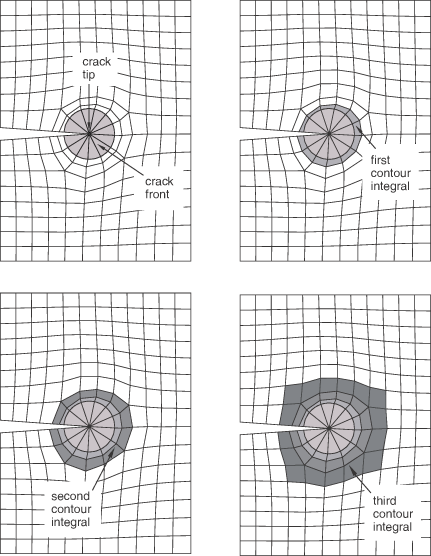
\includegraphics[width=\columnwidth]{contour_integral_regions_abaqus}}
\setbox2=\hbox{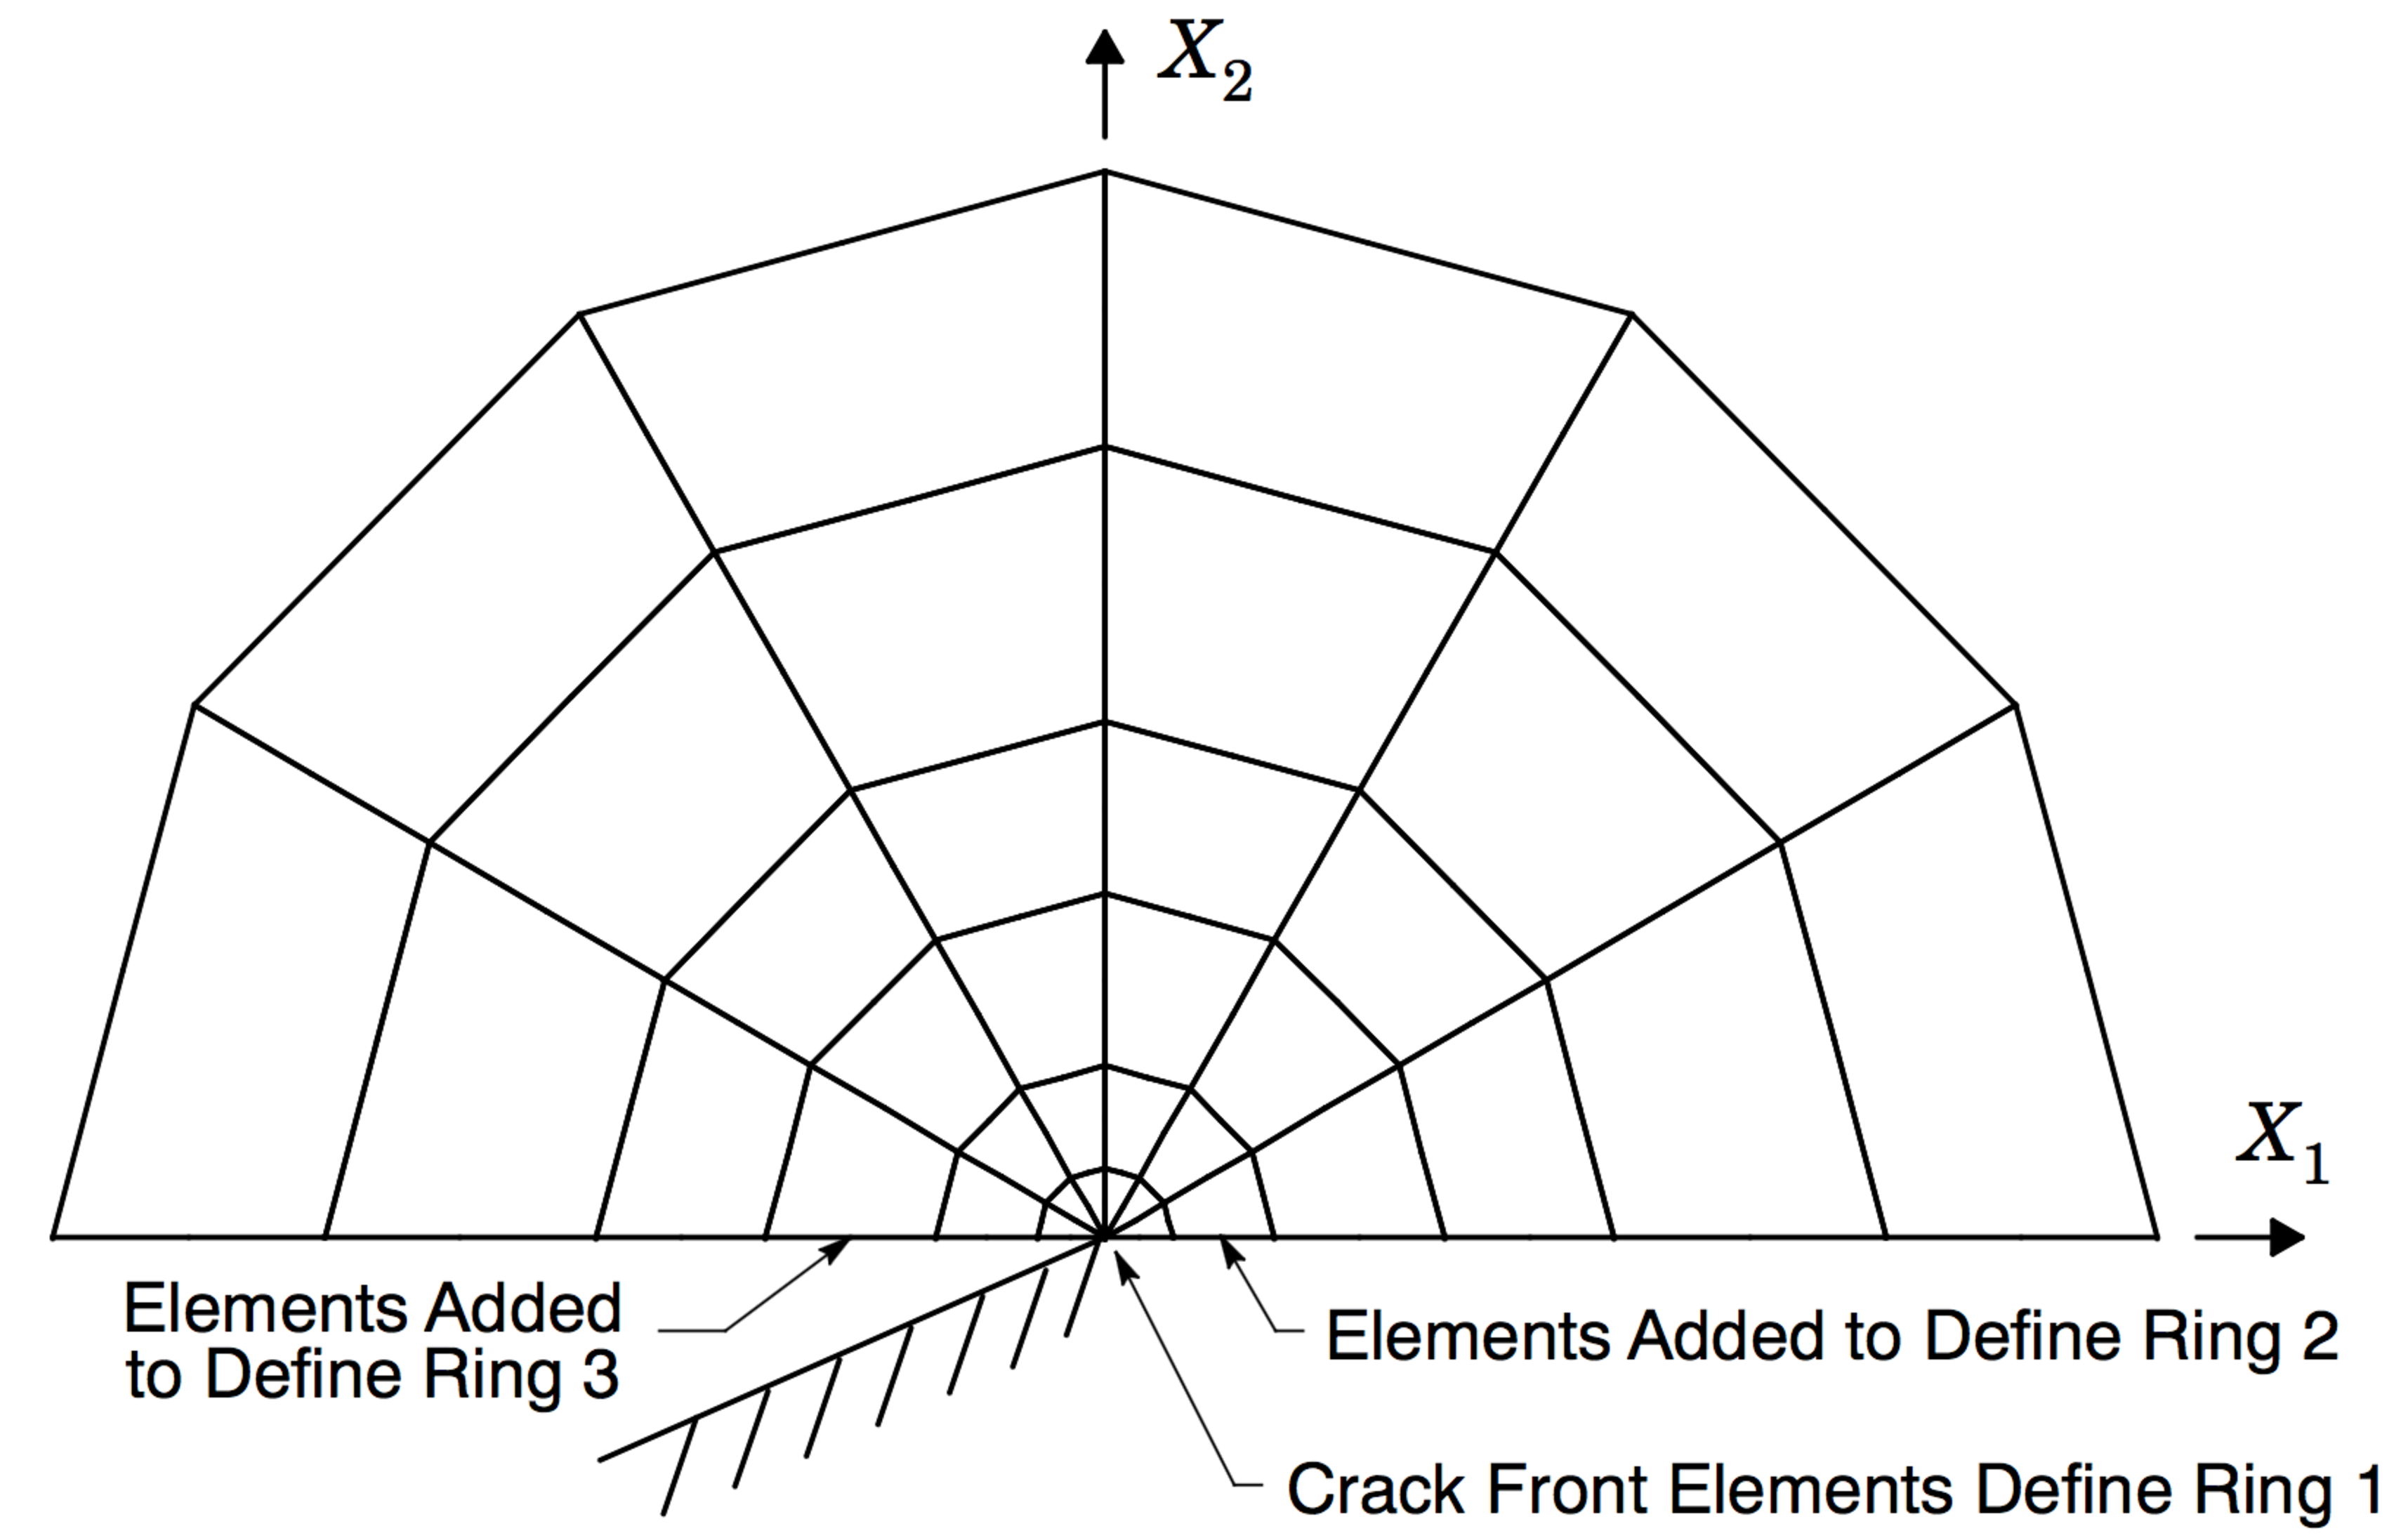
\includegraphics[width=\columnwidth]{contour_integral_regions_warp3d}}
\raisebox{0.5\ht1-0.5\ht2}{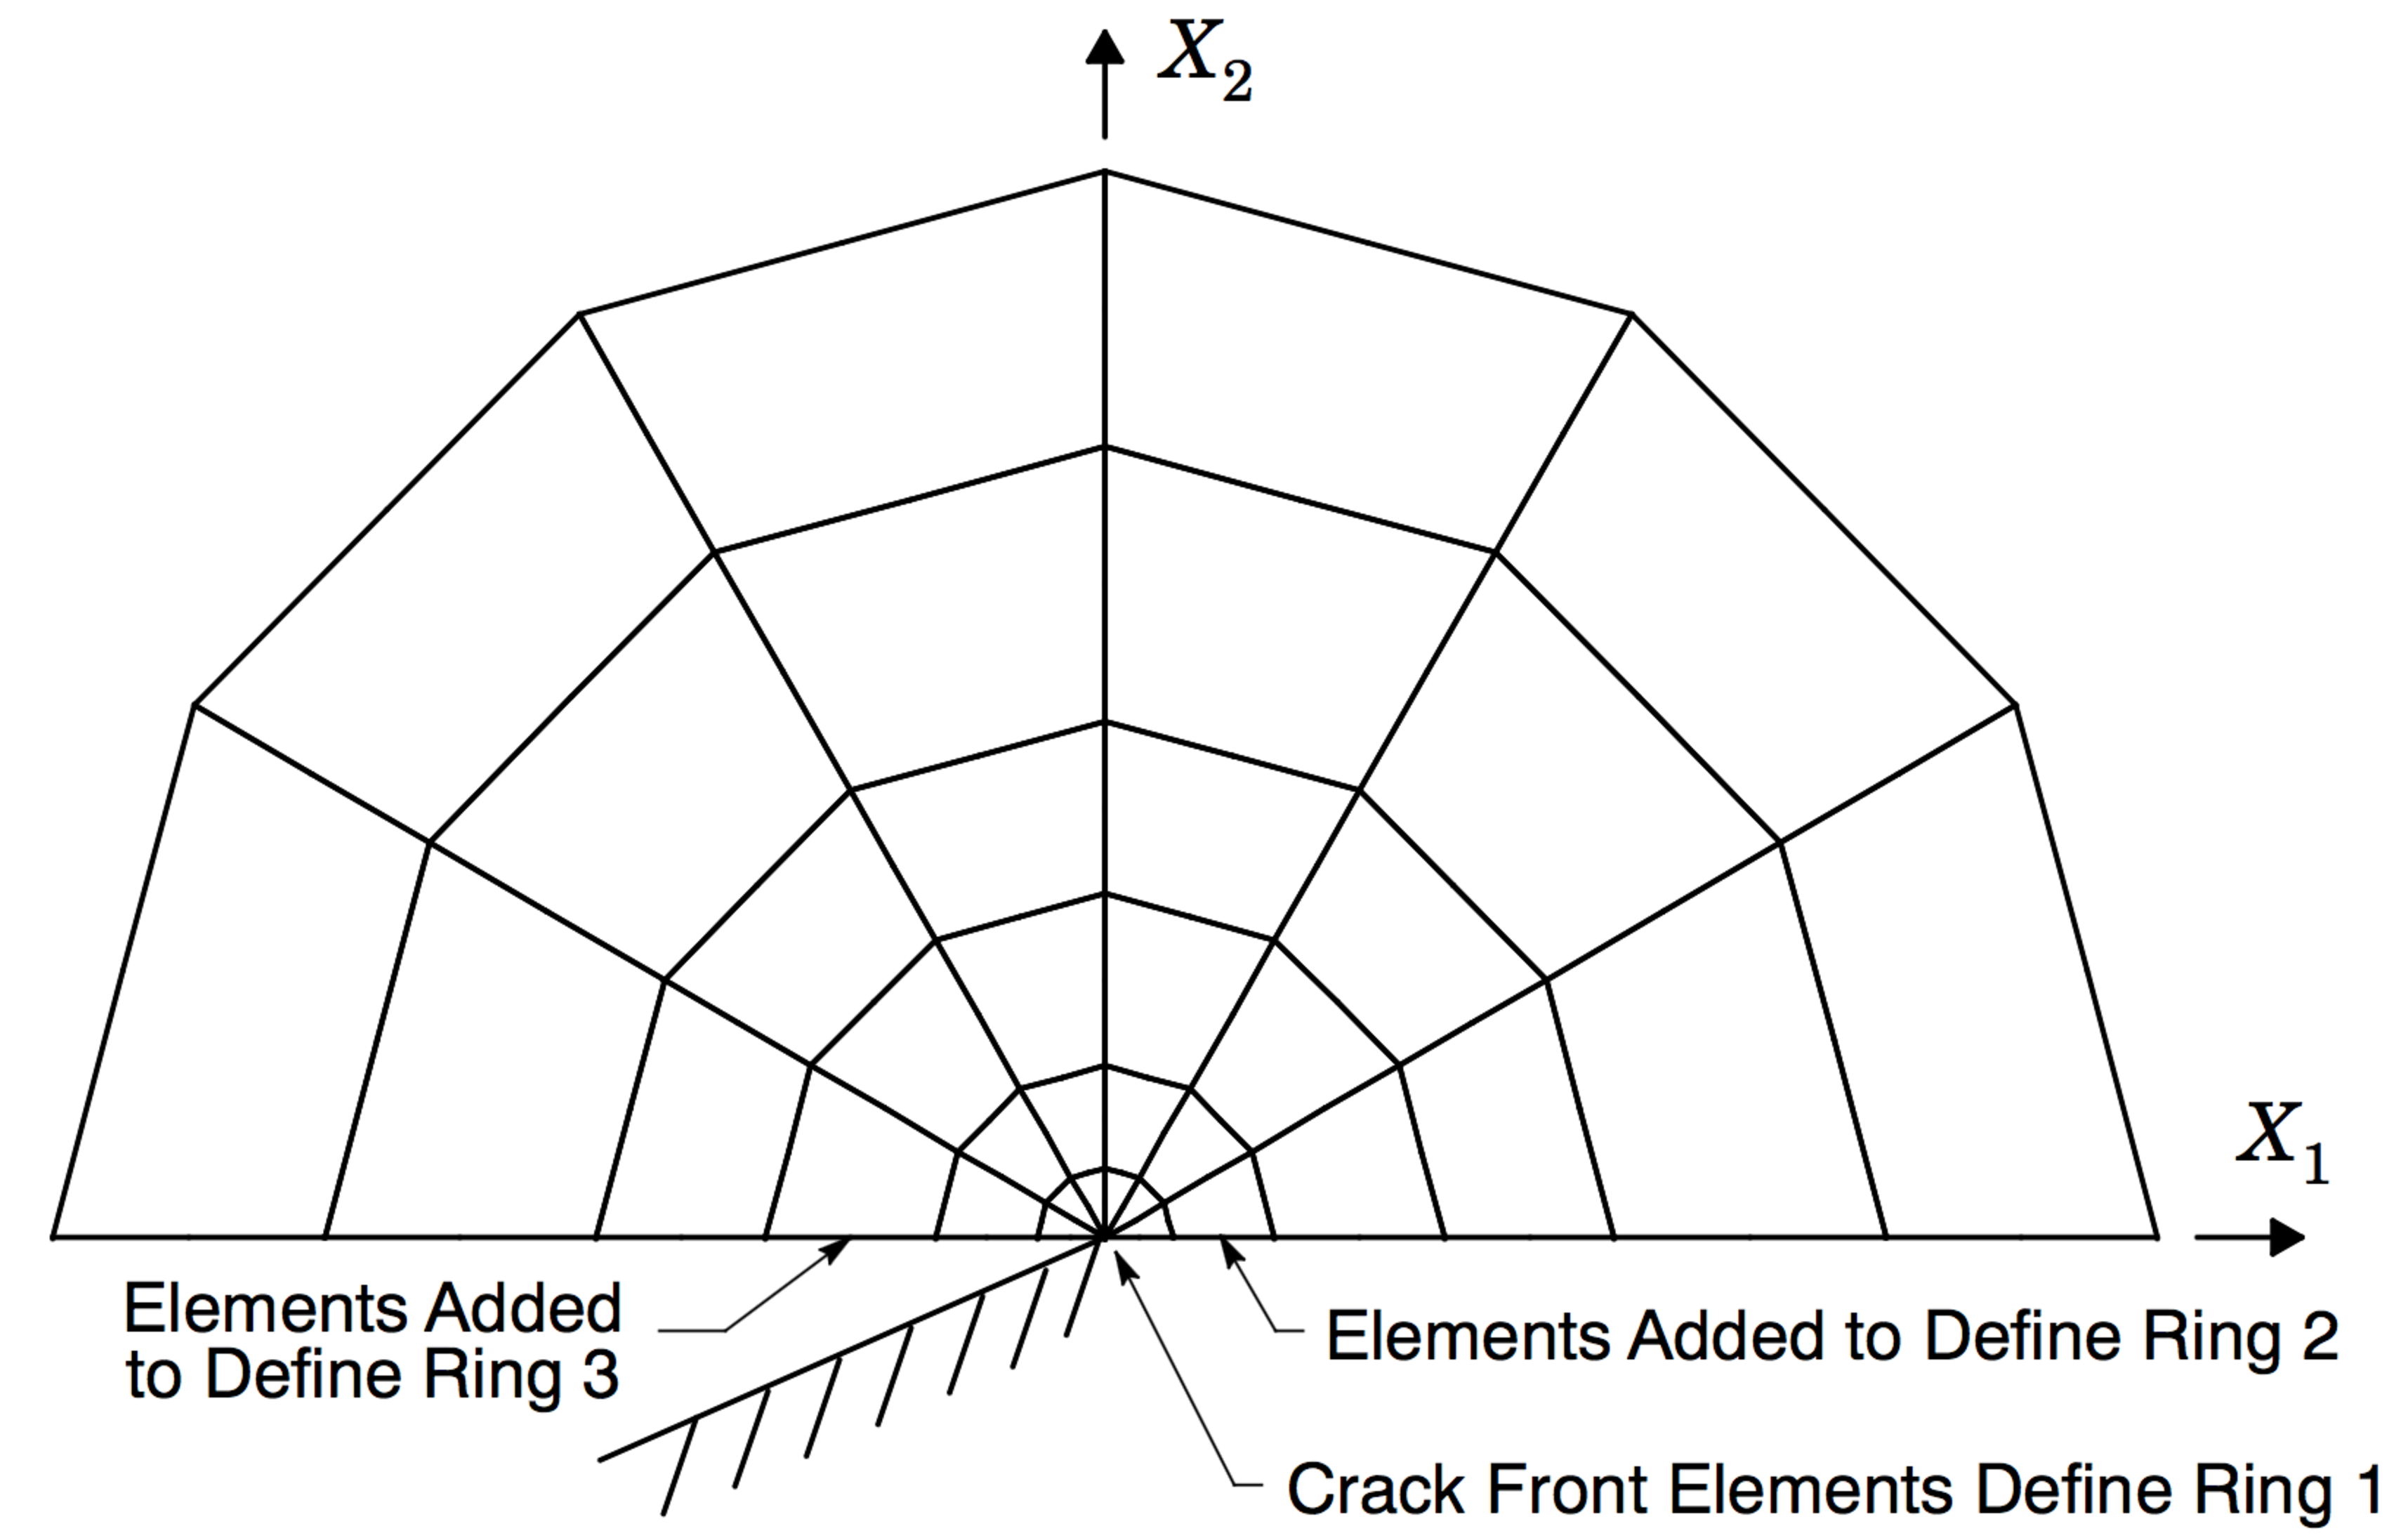
\includegraphics[width=\columnwidth]{contour_integral_regions_warp3d}}
\subcaption{WARP3D}
\end{minipage}
\begin{minipage}[b]{0.45\columnwidth}
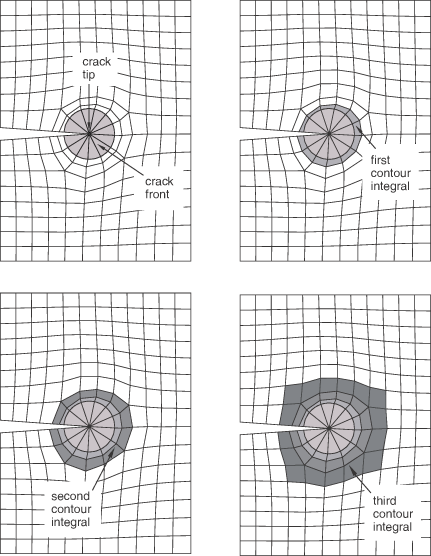
\includegraphics[width=\columnwidth]{contour_integral_regions_abaqus}
\subcaption{Abaqus}
\end{minipage}
\caption{\label{fig:fem-j-domains} Elements used in \J calculations}
\end{figure}

\begin{figure}[tbp]
\centering
\includegraphics[width=0.8\columnwidth]{{bend_ac02_at08_E0100_n20_wrp_J_converge_abs}}
\caption{\label{fig:J_convergence} Convergence of \J across 10 domains}
\end{figure}

\subsection{Addition of Elastic Boundary at Crack Face}
\label{sec:warp-elastic-boundary}

While examining the \J convergence data, some of the converged \J values had prominent minima at angles other than \(\phi=0{\SIUnitSymbolDegree}\) or \(\phi=90{\SIUnitSymbolDegree}\), for example, the values shown in \Cref{fig:negative_J} around \(\phi=70{\SIUnitSymbolDegree}\).
A more typical \((\phi, \J)\) graph with a minimum at  \(\phi=90{\SIUnitSymbolDegree}\) is shown in \Cref{fig:J_convergence}.
Further review of the model behavior revealed that the combination of particularly deep cracks and large \(\phi\) values showed positive \(z\) displacements, even at early load steps, as seen in \Cref{fig:positive-displacements}.
Typically, for models loaded in tension, this behavior never occurs: the symmetry plane condition for nodes outside the crack front fixes all those nodes at \(z=0\), and application of negative displacement boundary conditions (or the corresponding positive tensile stress) pulls the unconstrained nodes inside the crack front in the negative \(z\) direction.

But for models loaded in bending, elements near the uncracked face of the plate will be loaded in compression, and nodes will be pushed in the positive \(z\) direction.
Outside the crack front, the symmetry plane condition keeps nodes fixed at \(z=0\), exactly as in the tension model.
Inside the crack front, some nodes may be pushed across the \(z=0\) plane.

WARP3D supports the definition of unmeshed contact surfaces, either finite-sized rectangular planes, cylinders, or spheres.
Elements that intersect these contact surfaces have a penalty force applied to nodes, where the magnitude of the force is proportional to the nodes' penetration distance.
The common practice in finite element modeling would be use a perfectly rigid contact surface, or a contact body with an stiffness several orders of magnitude larger than the local stiffness of the meshed model in the contact region.

As WARP3D does not support perfectly rigid contact surfaces, a finite stiffness value must be selected.
This stiffness value should be a few orders of magnitude higher than the stiffness of elements making contact, but the element stiffnesses themselves are not constant.
An element with a cross sectional area \(A\), thickness \(L_\text{e}\), and elastic modulus \(E\) will have a stiffness of \(\frac{AE}{L_\text{e}}\).
For the set of models used in this research, elements near the crack front will have \(A\) on the order of \SI{1e-4} and \(L_\text{e}\) on the order of \SI{2e-3} or higher.
This places the element stiffness at least 1--2 orders of magnitude below \(E\).
Thus, the boundary stiffness was set to \(E\) for all 600 models.
%At first, stiffness values of either \(100 E\) or \(10 E\) were used, but models with particularly deep cracks would often fail to converge due to excessive node penetration and corresponding high penalty forces.
%One option to improve convergence would be to either use additional load steps, or to change the load time step during initial contact to reduce the penetration and penalty forces at those steps.
%Either of these options could require individual adjustment of up to 600 models, so another option was considered.
%
%Since the contact surface is intended to mimic the behavior of the opposite half of the cracked plate, and the contact surface occupies a fixed position in space, a contact surface stiffness of \(E\) was used.
%\todo{Did this just happen to work out? \(E\) isn't really a stiffness value, it's an elastic modulus. But if the effective local stiffness of the protruding cracked material was much less than \(E\), that's why it worked.}
The effects of this contact surface on \(z\) displacement can be seen in \Cref{fig:elastic-boundary-displacement}.
All nodes originally located on the \(z=0\) plane remain at or below the \(z=0\) plane when the elastic boundary is applied.

The effect on local \J values can be seen in \Cref{fig:elastic-boundary-J-CMOD}.
At \(\phi=0{\SIUnitSymbolDegree}\) and \(\phi=30{\SIUnitSymbolDegree}\), where the crack was already in tension, no effect can be seen.
But at \(\phi=90{\SIUnitSymbolDegree}\), \J values are 4--5 times lower due to the compressive stresses applied by the elastic boundary.
Additionally, the \J graphs no longer shows prominent minima at angles other than \(\phi=0{\SIUnitSymbolDegree}\) or \(\phi=90{\SIUnitSymbolDegree}\), as shown in \Cref{fig:elastic-boundary-J-phi}.
Even if the minimum \J value occurs at an angle other than \(\phi=90{\SIUnitSymbolDegree}\), all the \J values where the crack faces close are orders of magnitude lower than the highest \J values for the crack.

\begin{figure}[tbp]
\centering
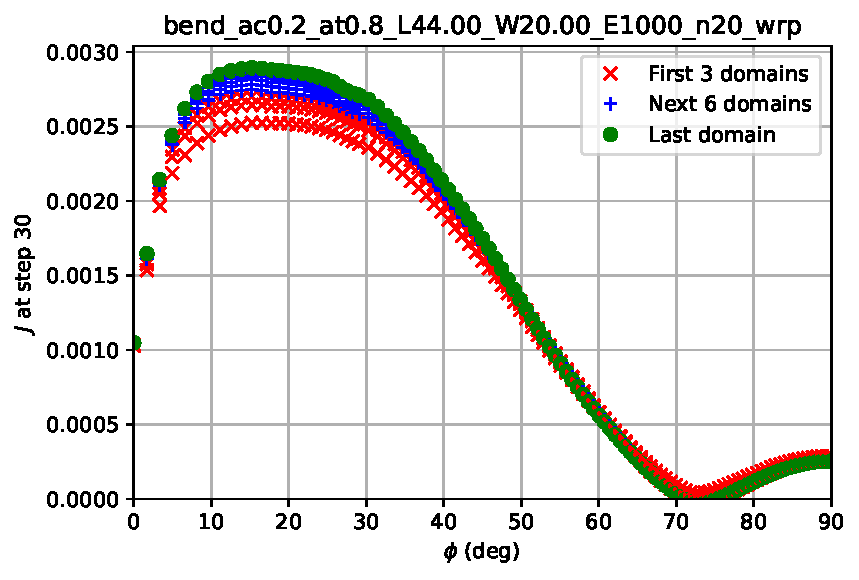
\includegraphics[width=0.8\columnwidth]{negative_J}
\caption{\label{fig:negative_J} Anomalous \J convergence graph}
\end{figure}

\begin{figure}[tbp]
\centering
\begin{minipage}{0.45\columnwidth}
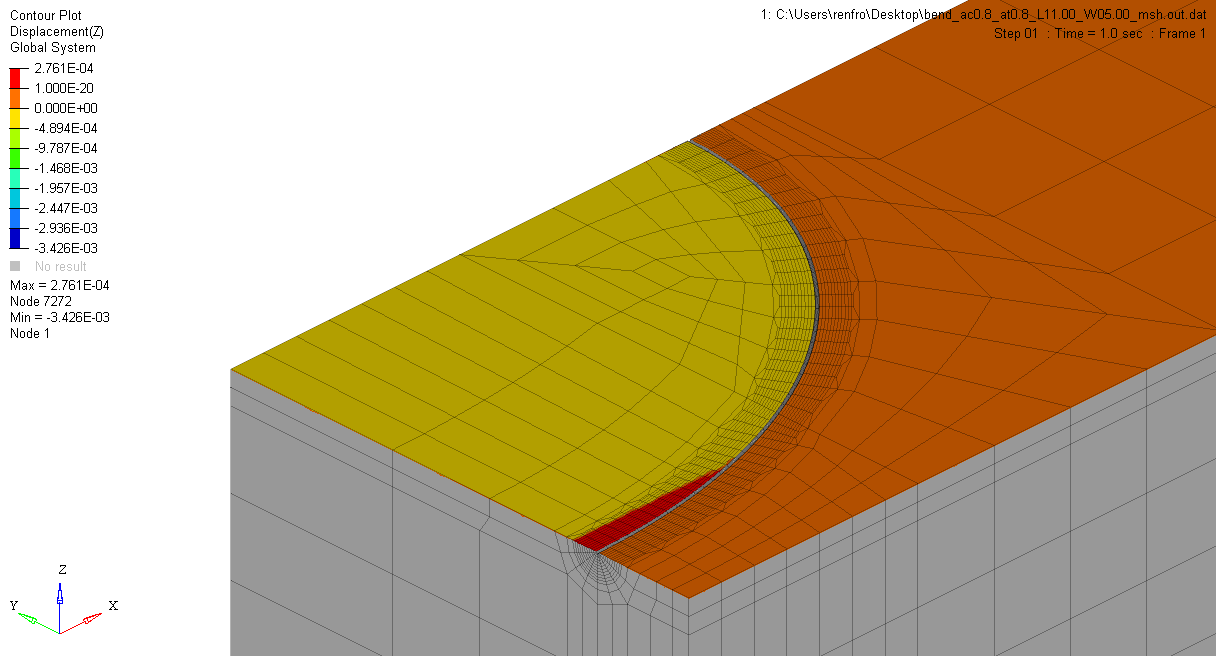
\includegraphics[width=\columnwidth]{step-01-zoomed}
\subcaption{First load step}
\end{minipage}
\begin{minipage}{0.45\columnwidth}
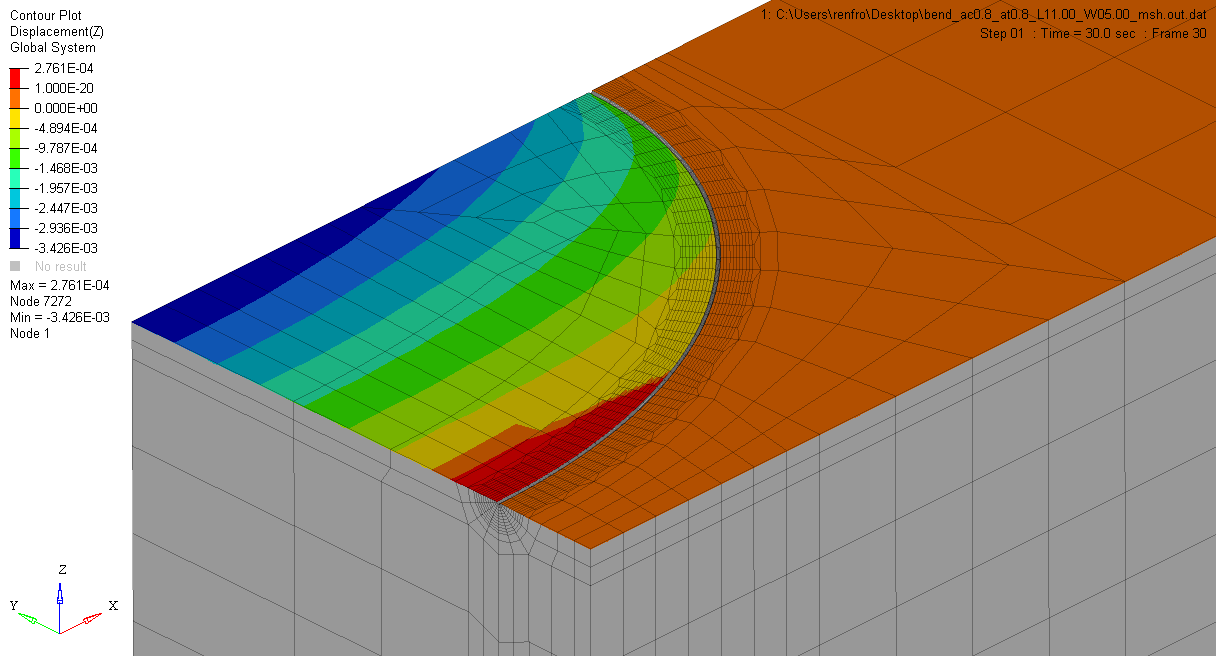
\includegraphics[width=\columnwidth]{step-30-zoomed}
\subcaption{Last load step}
\end{minipage}
\caption{\label{fig:positive-displacements} Example of model with positive \(z\) displacements at crack face}
\end{figure}

\begin{figure}[tbp]
\centering
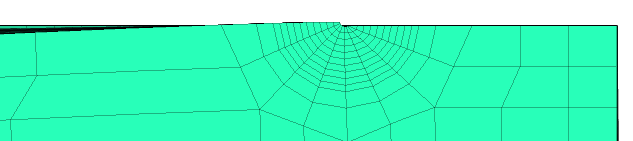
\includegraphics[width=\columnwidth]{left-step-30-10x-zoomed-before.png}
\subcaption{Before addition of elastic boundary}
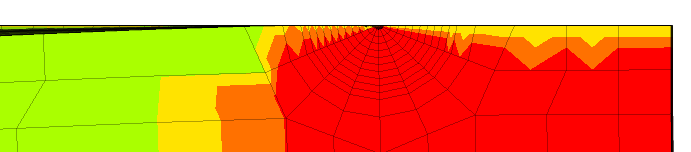
\includegraphics[width=\columnwidth]{left-step-30-10x-zoomed-after.png}
\subcaption{After addition of elastic boundary}
\caption{\label{fig:elastic-boundary-displacement} Effect of elastic boundary at crack face on \(z\) displacement (\(10\times\) scale factor)}
\end{figure}

\begin{figure}[tbp]
\centering
\begin{minipage}{0.45\columnwidth}
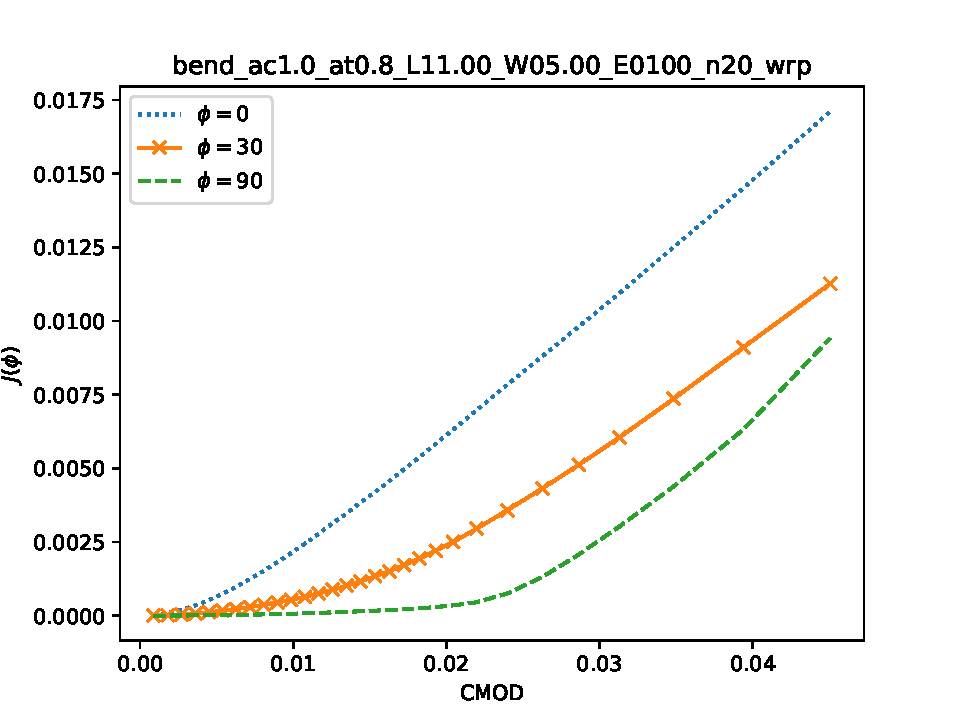
\includegraphics[width=\columnwidth]{before-J_CMOD_bend_ac10_at08_L1100_W0500_E0100_n20_wrp}
\subcaption{Before addition of elastic boundary}
\end{minipage}
\begin{minipage}{0.45\columnwidth}
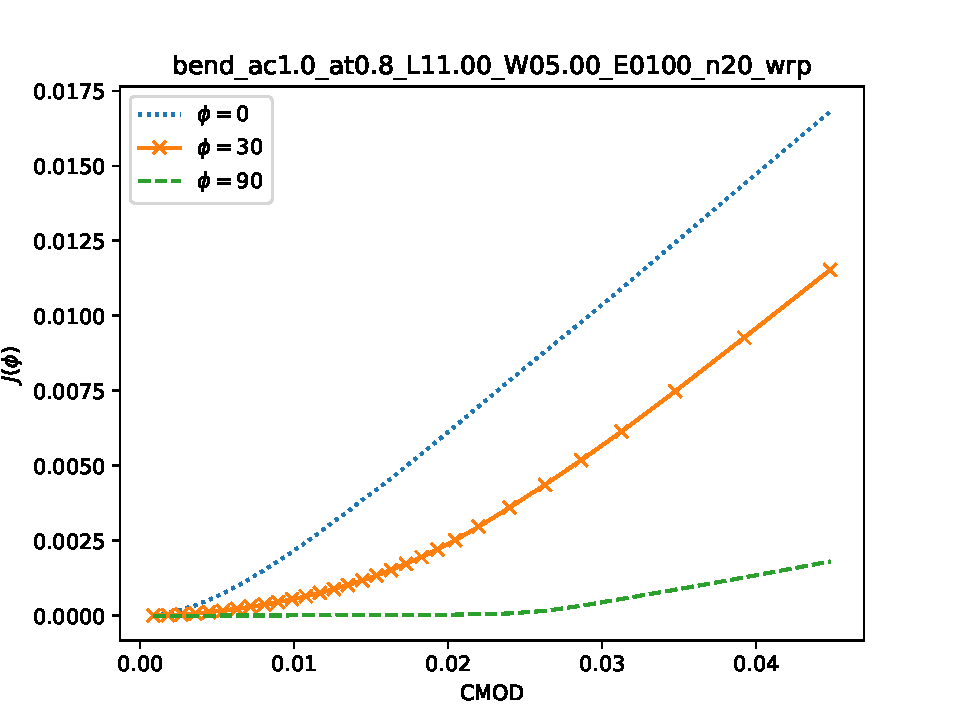
\includegraphics[width=\columnwidth]{after-J_CMOD_bend_ac10_at08_L1100_W0500_E0100_n20_wrp}
\subcaption{After addition of elastic boundary}
\end{minipage}
\caption{\label{fig:elastic-boundary-J-CMOD} Effect of elastic boundary at crack face on \J-CMOD relationship}
\end{figure}

\begin{figure}[tbp]
\centering
\begin{minipage}{0.45\columnwidth}
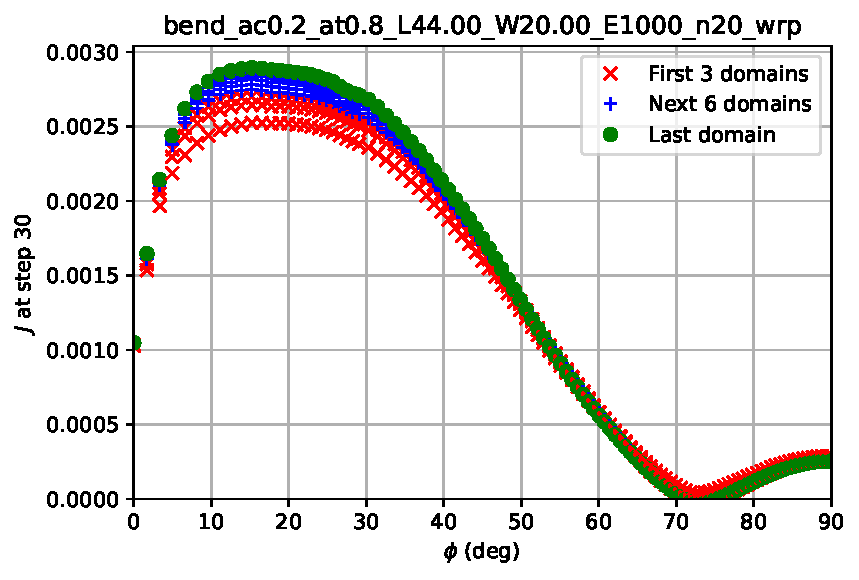
\includegraphics[width=\columnwidth]{negative_J}
\subcaption{Before addition of elastic boundary}
\end{minipage}
\begin{minipage}{0.45\columnwidth}
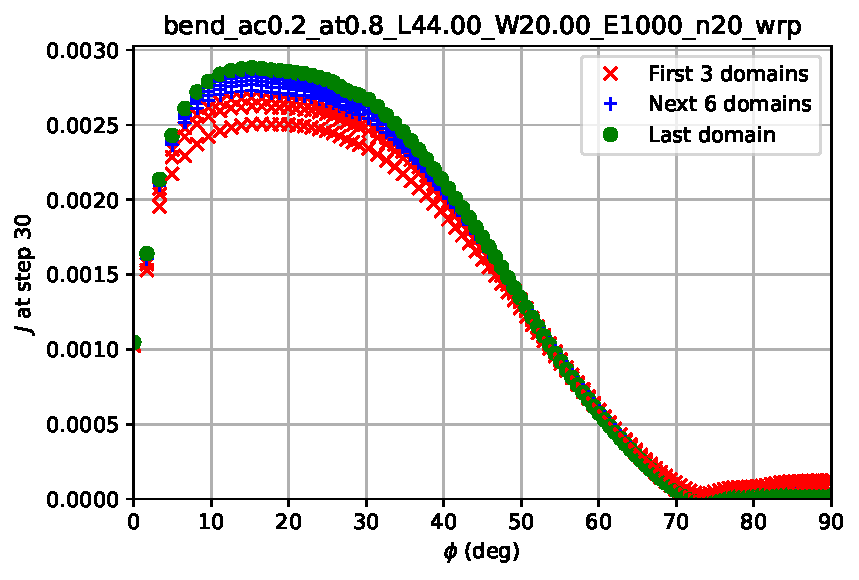
\includegraphics[width=\columnwidth]{negative_J_corrected}
\subcaption{After addition of elastic boundary}
\end{minipage}
\caption{\label{fig:elastic-boundary-J-phi} Effect of elastic boundary at crack face on \(\J-\phi\) relationship}
\end{figure}

\section{Extracting Results for TASC Interpolation Database}
\label{sec:postprocess}

Once \Cref{alg:optimize_bc} has applied a boundary condition value large enough to cause substantial elastic-plastic behavior and stable slopes in the later region of the \J-CMOD curve suitable for accurate linear extrapolation, the program can extract the results required by the TASC program using \Cref{alg:postprocess}.
Most of the tasks required for the extraction have already been demonstrated in \Cref{sec:solve}, as the model results are used to find the boundary conditions required to provide accurate linear extrapolations of the \J-CMOD curve.

\begin{algorithm}[tbp]
  \caption{Postprocess}
  \label{alg:postprocess}
  \begin{algorithmic}
    \Procedure{Postprocess}{input file}
    \State bpf file $\gets$ \Call{Get BPF Filename}{input file}
    \State results files $\gets$ \Call{Extract Results}{bpf file}
    \State \Comment{a dictionary containing names of reaction and displacement result files}
    \State node file $\gets$ \Call{Get Mesh Filename}{input file}
    \State reaction table $\gets$ \Call{Get Nodal Results}{reaction result filename}
    \State node table $\gets$ \Call{Get Node Coordinates}{node file}
    \State output file $\gets$ \Call{Get Output Filename}{input file}
    \State output lines $\gets$ read output file
    \State input lines $\gets$ read input file
	\State CMOD $\gets$ \Call{Get CMOD}{node table, displacement result filename, 0, 0, 0}
	\State $\phi$, \J $\gets$ \Call{Find \J}{input lines, output lines}
	%\State $\J(\phi=\frac{\pi}{6})$ $gets$ \Call{Interpolate \J}{$\phi$, \J, \frac{\pi}{6}}
	\State reaction $\gets$ reaction values at location $(y, z) = (0, -\frac{\Souter}{2})$
	\State \Comment{get reactions at outer roller location}
	\State displacement outer $\gets$ Average of displacement values at location $(y, z) = (0, -\frac{\Souter}{2})$
	\State \Comment{get average displacement of nodes at outer roller location (top of plate)}
	\State displacement inner upper $\gets$ Average of displacement values at location $(y, z) = (0, -\frac{\Sinner}{2})$
	\State displacement inner lower $\gets$ Average of displacement values at location $(y, z) = (-t, -\frac{\Sinner}{2})$
	\State \Comment{get average displacement of nodes at inner roller location (top and bottom of plate)}
	\State displacement inner $\gets$ $\frac{1}{2}$(displacement inner upper + displacement inner lower)
	\State moment arm $\gets$ $\frac{\Souter}{2} -$ (displacement inner - displacement outer)
	\State \Comment{moment arm is distance from averaged inner roller nodes to averaged outer roller nodes}
	\State Create MATLAB .mat file containing $\phi$, \J, CMOD, reaction, moment arm, BPF filename
    \EndProcedure
  \end{algorithmic}
\end{algorithm}
